% Geometry setup
\documentclass[a4paper]{article}
\usepackage[margin=1.5cm]{geometry}

% Language setup
\usepackage[T1]{fontenc} % Output character encoding
\usepackage[utf8]{inputenc} % Input character encoding

% Spacing setup
\setlength{\parindent}{0pt} % No paragraph indenting
\setlength{\parskip}{5pt} % Set spacing between paragraphs
\frenchspacing
\newcommand{\rmspace}{\vspace{-19pt}}

% Dependency setup
\usepackage{amsmath}
\usepackage{amssymb}
\usepackage{amsfonts}
\usepackage{mathtools}
\usepackage{dsfont}
\usepackage{listings}
\usepackage{float}
\usepackage{graphicx}
\usepackage{hyperref}
\usepackage{url}
\usepackage[comma,authoryear]{natbib}
\usepackage[shortlabels]{enumitem}
\usepackage{minted}
\usepackage{makecell}

\DeclarePairedDelimiter{\ceil}{\lceil}{\rceil}

% Code pretty print
\usepackage{minted}

% Hyperlink format
\usepackage{xcolor}
\hypersetup{
    colorlinks,
    linkcolor={red!50!black},
    citecolor={blue!50!black},
    urlcolor={blue!80!black}
}

% Title setup
\author{Viktória Nemkin (nemkin@cs.bme.hu)}
\title{Practice Session Notes: Theory of Algorithms}

% Custom commands
\newcommand{\lineparagraph}[1]{\paragraph{#1}\mbox{}\\}
\newcommand{\titlemath}[1]{\texorpdfstring{#1}{Lg}}
\newcommand{\separate}{\vspace{2mm}\hrulefill{}\vspace{2mm}}
\newcommand{\condition}{\text{, }~}

% Supress warnings
\hbadness=99999 % Underfull hbox

% Document
\begin{document}
\maketitle

These, are my practice session notes, they are based on my personal notes and on the Hungarian course's solutions, found here under the heading \textbf{''A gyakorlatokon használt feladatsorok''}:\\ \url{http://www.cs.bme.hu/~csima/algel2020/index_2020_tavasz_vegleges.html} $\rightarrow$ In the case of hashings, this guide uses open hashings with quadratic probing by starting from the left, while we start that one to the right. Check Session 13, Exercise 9 for details!

This is a work in progress, I am updating these whenever I have time.

\textbf{Mistakes are possible}, if you spot any or if you have any questions about these notes, please contact me at nemkin@cs.bme.hu or in MS Teams.

\textbf{Version log}: \href{https://github.com/nemkin/thalg-notes/commits/main}{https://github.com/nemkin/thalg-notes/commits/main} - So you can check what was updated and when. (Or send me a PR if you find any errors? :) )

\tableofcontents
\pagebreak

\section{February 16th (Session 1): O, \titlemath{$\Omega$, $\Theta$}, pattern matching}
\subsection{Session 1, Exercise 01}

\lineparagraph{Exercise}

There are two algorithms for the same problem, $A$ and $B$. Let the functions describing their worst case running times be $f_A$ and $f_B$. It is known that $f_A(n) = O(f_B(n))$. Does it follow that...

\begin{enumerate}[a.)]
\item $A$ is faster on every input than $B$?
\item except for finitely many inputs $A$ is faster than $B$?
\item for large enough inputs $A$ is faster than $B$?
\end{enumerate}

\lineparagraph{Solution}
\pagebreak
\subsection{Session 1, Exercise 2}

\lineparagraph{Exercise}

Which of the following functions are $O(n^2)$ and which are $\Omega(n^2)$?

\begin{enumerate}[a.)]
\item $f_1(n) = 11n^2 + 100000$
\item $f_2(n) = 8n^2\log_2(n)$
\item $f_3(n) = 1.5n + 3\sqrt{n}$
\end{enumerate}

\lineparagraph{Solution}

Definitions:

\begin{itemize}
    \item $f(n)\in{}O(g(n))$ if there exists $c>0$ and $n_0\in{}\mathds{Z^+}$ so that $f(n) \leq{} cg(n)$ for $\forall{}n\geq{}n_0$.
    \item $f(n)\in{}\Omega(g(n))$ if there exists $c>0$ and $n_0\in{}\mathds{Z^+}$ so that $f(n)\text{ }\color{red}\mathbf{\geq{}}\color{black} cg(n)$ for $\forall{}n\geq{}n_0$.
\end{itemize}

To prove that something is $\in{}O(g(n))$ or $\in{}\Omega(g(n))$, give one $c$ and $n_0$ and show that the above requirement is holds true.

To prove that something is not $\in{}O(g(n))$ or $\in{}\Omega(g(n))$, prove that no possible $c$ and $n_0$ combination would make the above requirement hold true.

Fist look at the given function, and figure out whether you think the definition is true or not and then based on that choose the appropriate proof.

\textbf{a)}

$f(n) = 11n^2 + 100000$.

Gut feeling: The most significant component here is $n^2$, so we believe it is asymptotically similar to $n^2$, so both $f(n)\in{}O(n^2)$ and $f(n)\in{}\Omega(n^2)$.

First let's show that $f(n)\in{}O(n^2)$:

Start from the function and give \textbf{upper} bounds until we reach something in the form of $\text{const}*n^2$.

$f(n) = 11n^2 + 10^5 \leq{} 12n^2$ if $n^2 \geq{} 10^5$, or $n \geq{} 10^{5/2}$, where we can be generous and just say $n \geq{} 1000$, since it is not necessary to find the smallest possible $n_0$, only one sufficient.

We have arrived at: $f(n) \leq{} 12n^2$ if $n\geq{}1000$.

Then by choosing $n_0=1000$ and $c=12$, this turns into $f(n) \leq{} cn^2$ if $n\geq{}n_0$, which by definition means that $f(n) \in{} O(n^2)$.

Now let's show that $f(n)\in{}\Omega(n^2)$:

Start from the function again, however now we give \textbf{lower} bounds until we reach something in the form of $\text{const}*n^2$.

$f(n) = 11n^2 + 10^5 \geq{} 11n^2$, since $10^5\geq{}0$.

We have arrived at: $f(n) \geq{} 11n^2$. Now $c=11$, and there was no requirement for $n$, so we can choose $n_0=1$, and then this turns into $f(n) \geq{} cn^2$ if $n\geq{}n_0$, which by definition means that $f(n)\in{}\Omega(n^2)$.

Note:
\begin{itemize}
    \item Since we have shown that $f(n)\in{}O(n^2)$ and also $f(n)\in{}\Omega(n^2)$, the combination of the two is that $f(n)\in{}\Theta(n^2)$, so $11n^2+100000$ and $n^2$ are asymptotically similar.
\end{itemize}

\textbf{b)}

$f(n) = 8n^2\log_2(n)$

Gut feeling: This is going to be asymptotically bigger than $n^2$, since it is also multiplied with $\log_2(n)$. So we believe $f(n)\in{}\Omega(n^2)$, however $f(n)\notin{}O(n^2)$.

Let's start with showing that $8n^2\log_2(n)\notin{}O(n^2)$:

In this case we want to show that there is no possible choice of $c$ and $n_0$, which is done using indirect proof and arriving at a contradiction.

Let's indirectly state that $8n^2\log_2(n)\in{}O(n^2)$, which is equivalent to saying:

There exists some $c>0$ and $n_0\in{}\mathds{Z^+}$ constants, so that

$8n^2\log_2(n) \leq{} cn^2$ for $\forall n\geq{}n_0$.

Let's divide the left and the righthand side with $n^2$:

$8\log_2(n) \leq{} c$ for $\forall n\geq{}n_0$.

Let's move the $8$ to the right:

$\log_2(n) \leq{} \frac{c}{8}$ for $\forall n\geq{}n_0$.

And this is a contradiction, since $\frac{c}{8}$ is a constant, while $\log_2(n)$ can be arbitrarily large for a given $n\geq{}n_0$, and we cannot give an upper bound to something arbitrarily large with a constant.

This means that the indirect statement was wrong so that $8n^2\log_2(n)\notin{}O(n^2)$.

Now let's show that $f(n)\in{}\Omega(n^2)$:

Start from the function again and give \textbf{lower} bounds until we reach something in the form of $\text{const}*n^2$.

$f(n) = 8n^2\log_2(n) \geq{} 8n^2$ when $n\geq{}2$, since $\log_2(n) \geq{} 1$ when $n\geq{}2$.

We have arrived at $f(n) \geq{} 8n^2$ when $n\geq{}2$, so we can choose $c=8$ and $n_0=2$, which gives $f(n) \geq{} cn^2$ when $n\geq{}n_0$, which is the definition of $f(n)\in{}\Omega(n^2)$.

\textbf{c)}

$f(n) = 1.5n + 3\sqrt{n}$

Gut feeling: This is going to be asymptotically smaller than $n^2$, since the most significant component is only $n$. So we believe $f(n)\in{}O(n^2)$, however $f(n)\notin{}\Omega(n^2)$.

Let's show that $f(n)\in{}O(n^2)$:

Start from the function and give \textbf{upper} bounds until we reach something in the form of $\text{const}*n^2$. (Actually, in this case, an even stonger statement will be made.)

$f(n) = 1.5n + 3\sqrt{n} \leq{} 4.5n$, since $\sqrt{n} \leq{} n$ (for $n\geq{}1$, which is a given).

We have arrived at $f(n) \leq{} 4.5n$, which means that $c=4.5$ and since there is no lower bound on $n$, we can choose $n_0=1$, to turn it into $f(n) \leq{} cn$ for $\forall{}n\geq{}n_0$, which means by definition that $f(n)\in{}O(n)$. 

Now since we know that $O(n)\subset{}O(n^2)$, this also proves that $f(n)\in{}O(n^2)$.

Let's continue with showing that $1.5n + 3\sqrt{n}\notin{}\Omega(n^2)$:

In this case we want to show that there is no possible choice of $c$ and $n_0$, which is done using indirect proof and arriving at a contradiction.

Let's indirectly state that $1.5n + 3\sqrt{n}\in{}\Omega(n^2)$, which is equivalent to saying:

There exists some $c>0$ and $n_0\in{}\mathds{Z^+}$ constants, so that

$1.5n + 3\sqrt{n} \geq{} cn^2$ for $\forall n\geq{}n_0$.

How we handle this situation is by giving something that is larger than $1.5n + 3\sqrt{n}$ and show that even this larger thing still cannot upper bound $cn^2$, so the smaller, original function can not either:

Borrowing from the previous proof, we know that $4.5n \geq{} 1.5n + 3\sqrt{n}$:

$4.5n \geq{} 1.5n + 3\sqrt{n} \geq{} cn^2$ for $\forall n\geq{}n_0$.

Now let's just look at the two sides:

$4.5n \geq{} cn^2$ for $\forall n\geq{}n_0$.

Let's divide both sides by $n$:

$4.5 \geq{} cn$ for $\forall n\geq{}n_0$.

And move the constant to the left:

$\frac{4.5}{c} \geq{} n$ for $\forall n\geq{}n_0$.

And here is the contradiction: this can not be true, since $n$ is arbitrarily large, while it should be upper bound by a constant: $\frac{4.5}{c}$. This shows that $4.5n$ can not be an upper bound for $cn^2$, so an even smaller function, $1.5n + 3\sqrt{n}$ definitely can't be either for any given $c$ and $n_0$ pair.\pagebreak
\subsection{Session 1, Exercise 03}

\lineparagraph{Exercise}

For which integers $a,b > 1$ do the following hold true?

\begin{enumerate}[a.)]
\item $n^a = O(n^b)$
\item $2^{an} = O(2^{bn})$
\item $\log_a(n) = O(\log_b(n))$
\end{enumerate}

\lineparagraph{Solution}
\pagebreak
\subsection{Session 1, Exercise 04}

\lineparagraph{Exercise}

Put the following functions in order of non-decreasing order of magnitude, i.e., if $f_i$ is immediately followed by $f_j$, then $f_i(n) = O(f_j(n))$ holds.

\begin{enumerate}[a.)]
\item $f_1(n) = 8n^3$
\item $f_2(n) = 5\sqrt{n} + 1000n$
\item $f_3(n) = 2^{(\log_{2}n)^2}$
\item $f_4(n) = 1514n^{2}\log_{2}n$
\end{enumerate}

\lineparagraph{Solution}
\pagebreak
\subsection{Session 1, Exercise 05}

\lineparagraph{Exercise}

Give $O$ bounds for the following functions:

\begin{enumerate}[a.)]
    \item $(n^2+8)(n+1)$
    \item $(n\log{n} + n^2)(n^3+2)$
    \item $(n!+2^n)(n^3+\log(n^2+1))$
    \item $(2^n+n^2)(n^3+3^n)$
\end{enumerate}

\lineparagraph{Solution}
\pagebreak
\subsection{Session 1, Exercise 06}

\lineparagraph{Exercise}

Let $f_1(n) = 1.5n!$ and $f_2(n)=200(n-1)!$. Which of the following is true?

\begin{enumerate}[a.)]
    \item $f_1=O(f_2)$
    \item $f_2=O(f_1)$
    \item $f_1=\Omega(f_2)$
    \item $f_2=\Omega(f_1)$
\end{enumerate}

\lineparagraph{Solution}

$n! = n(n-1)!$, so we can already see that $f_1(n) \approx nf_2(n)$.

Let's prove that $f_2 \in{} O(f_1)$:

$f_2(n) = 200(n-1)! \leq{} 200n(n-1)! = 200n! = \frac{200}{1.5}1.5n! = \frac{200}{1.5}f_1(n)$. So $c=\frac{200}{1.5}$ and $n_0=1$ works.

Let's also prove that $f_1 \notin{} O(f_2)$, $1.5n! \notin{} O(200(n-1)!)$.

Let's assume indirectly that $1.5n! \in{} O(200(n-1)!)$.

That means that there exists $c>0$ and $n_0\in{}\mathds{Z}^+$ such that

$1.5n! \leq{} c200(n-1)!$ for $\forall{}n\geq{}n_0$.

Let's use $n!=n(n-1)!$:

$1.5n(n-1)! \leq{} c200(n-1)!$ for $\forall{}n\geq{}n_0$.

Let's divide by $(n-1)!$:

$1.5n \leq{} c200$ for $\forall{}n\geq{}n_0$.

And move the constants to the right:

$n \leq{} c\frac{200}{1.5}$ for $\forall{}n\geq{}n_0$.

This is a contradiction, since we would want to upper bound $n$ with a constant, however $n$ can be arbitrarily large.

Thus the indirect statement is false, the original statement is true, so $f_1 \notin{} O(f_2)$.

Let's look at the questions now:

\begin{enumerate}[a.)]
    \item $f_1=O(f_2)$, we proved this to be false.
    \item $f_2=O(f_1)$, we proved this to be true.
    \item $f_1=\Omega(f_2)$, this is true, because $f_2=O(f_1)$ implies that $f_1=\Omega(f_2)$.
    \item $f_2=\Omega(f_1)$, this is false, because this would imply $f_1=O(f_2)$, which is false.
\end{enumerate}


Note:
\begin{itemize}
    \item It is very important to not only prove that $f_2 \in{} O(f_1)$, but also separately prove that $f_1 \notin{} O(f_2)$, since both $f_2 \in{} O(f_1)$ and $f_1 \in{} O(f_2)$ could be true, for example in the case of $f_1 = f_2$.
    \item $f\in{}O(g)$ implies that $g\in{}\Omega(f)$, since both definitions require us to come up with a $c$ and an $n_0$ and if we used the same $n_0$s and $c_2 = \frac{1}{c_1}$ or the reciprocal of the constants we can quickly arrive at $g\in{}\Omega(f)$ from $f\in{}O(g)$.
\end{itemize}\pagebreak
\subsection{Session 1, Exercise 07}

\lineparagraph{Exercise}

Let $L(n)$ denote the worst case running time of an algorithm on an input of length $n$. What can be said about the order of magnitude of function $L(n)$ if $L(1) = 2$ holds and for $n>1$ we have:

\begin{enumerate}[a.)]
    \item $L(n) = L(n-1) + 3$
    \item $L(n) = L(n-1) + 5$
    \item $L(n) = L(n-1) + 3n$
    \item $L(n) = 2L(n-1) + 3$
    \item $L(n) = L(\ceil*{\frac{n}{2}}) + 3$
    \item $L(n) = L(\ceil*{\frac{n}{2}}) + n^k$
    \item $L(n) = 2L(\ceil*{\frac{n}{2}}) + 3$
    \item $L(n) = 4L(\ceil*{\frac{n}{2}}) + 3$
\end{enumerate}

\lineparagraph{Solution}
\pagebreak
\subsection{Session 1, Exercise 08}

\lineparagraph{Exercise}

Using first Simple search, then Quick search determine how many times pattern $M = ABABC$ does occur in text $S = ABBABACABCBAC$. How many comparisons are made in each case?

\lineparagraph{Solution}


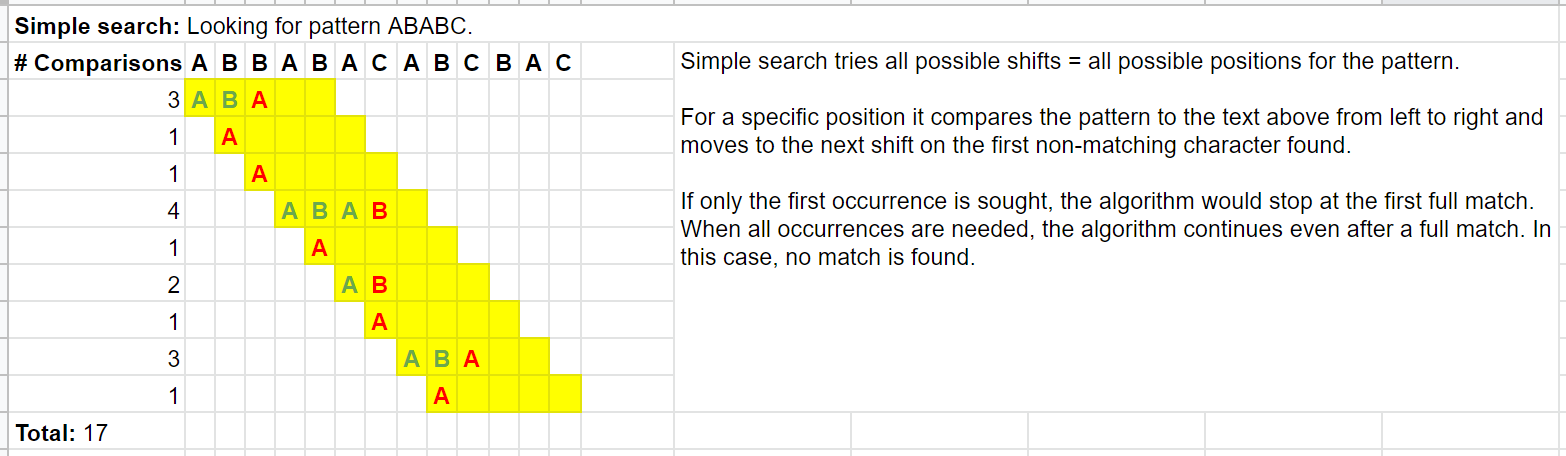
\includegraphics[width=\linewidth]{01/simple_search.png}

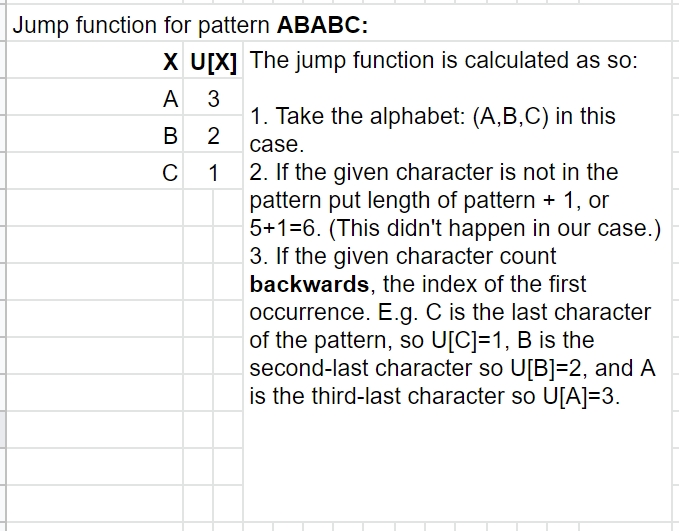
\includegraphics[width=0.5\linewidth]{01/jump_function.png}

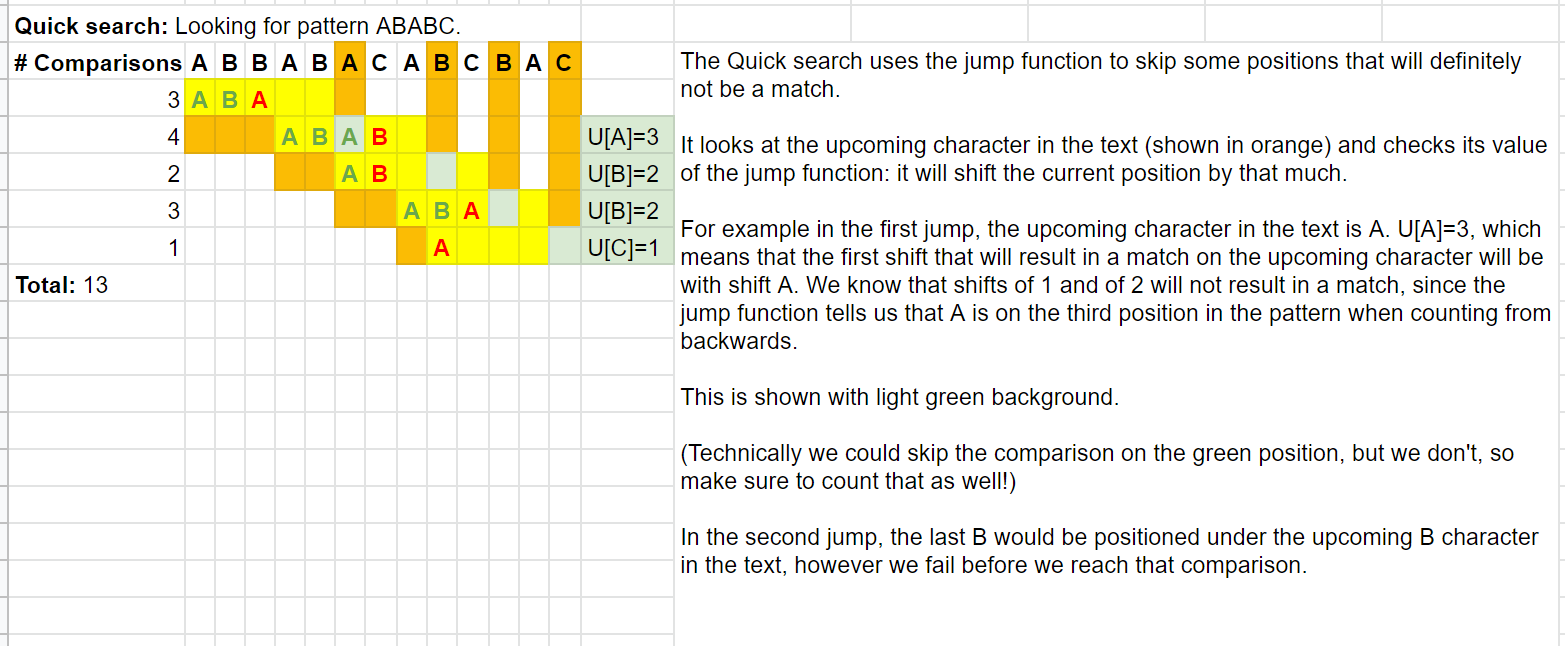
\includegraphics[width=\linewidth]{01/quick_search.png}\pagebreak
\subsection{Session 1, Exercise 9}

\lineparagraph{Exercise}

Let both the pattern and the text consist of only $0$'s, let the length of the pattern be $m$, while that of the text be $n$. How many comparisons are done...

\begin{enumerate}[a.)]
    \item by Simple search if only the first occurrence of the pattern is sought?
    \item by Simple search if all occurrences of the pattern are needed?
    \item by Quick search if only the first occurrence of the pattern is sought?
    \item by Quick search if all occurrences of the pattern are needed?
\end{enumerate}

\lineparagraph{Solution}

\begin{enumerate}[a.)]
    \item $m$, since the first position is immediately a match.
    \item All positions match. There are $n-m+1$ positions, the pattern will be checked on all characters, so $m(n-m+1)$.
    \item $m$, since the first position is immediately a match.
    \item All positions match. There are $n-m+1$ positions, the pattern will be checked on all characters, so $m(n-m+1)$.
\end{enumerate}

Note:
\begin{itemize}
    \item In this case there is no difference between what Simple search and what Quick search does. Quick search is able to skip \textbf{some} definitely non-matching positions based on a heuristic. In this case, all positions match, there is nothing to skip.
\end{itemize}
\pagebreak
\subsection{Session 1, Exercise 10}

\lineparagraph{Exercise}

Give text $S$ of length $n$ such that for a pattern consisting of $m>2$ $0$'s Simple search uses $O(n)$ comparisons on $S$, independently of $m$.

\lineparagraph{Solution}

If the first character doesn't match every position will fail after $1$ comparison. There will be $n-m+1$ positions, which is $O(n)$, because $n-m+1 \leq{} n+1 \leq{} n+n \leq{} 2n$, constants $c=2$, $n_0=1$ work.

So let's make a text in which no character is a $0$, e.g. all characters are $1$'s, so the first $0$ of the pattern will never match.\pagebreak
\subsection{Sesssion 1, Exercise 11}

Note: this is a hard exercise, using probability theory as well, it is not included in the exam!

\lineparagraph{Exercise}

Prove that the expected running time of Simple search is $O(n)$, when both the text and pattern are random $0$ - $1$ sequences (the bits are independent of each other and probabilities of $0$ and $1$ are both $\frac{1}{2}$). What happens if only the pattern is random?

\lineparagraph{Solution}

The pattern is denoted by $M$ and its length is $m=|M|$, the text is denoted by $S$ and its length is $n=|S|$.

Let's denote with the random variable $t_i$ the number of comparisons made by the Simple search algorithm for a pattern position with a shift of $i$ number of characters.

Then, in total the number of comparisons made is $\sum\limits_{i=0}^{n-m}t_i$, so the expected number of comparisons is $E(\sum\limits_{i=0}^{n-m}t_i)$.

$E(\sum\limits_{i=0}^{n-m}t_i) = \sum\limits_{i=0}^{n-m}E(t_i)$, due to the Linearity of Expectation. It is important to remember, that this holds true even when the variables are correlated, like in our case!

Now, the only thing left to find is $E(t_i)$.

For a given position $k$ in the pattern, the probability of it matching the current position in the text, or $P(S[k+i] = M[k])$ is $\frac{1}{2}$, since both the pattern and the text is random, and they match for $S[k+i] = M[k] = 0$ and $S[k+i] = M[k] = 1$ while not match for $S[k+i] = 0, M[k] = 1$ and $S[k+i] = 1, M[k] = 0$, all four of these happen with $\frac{1}{4}$ probability, and two of these are the desired.

Now, the comparisons are made up until the point one of them fails, and we care about the number of them. This would be a geometric distribution, if the number of possible positions would be infinite. While this is not true, since the pattern and the text are both finite, since we only care about an upper bound, we can over-estimate the expectation value with the geometric distribution's expectation value.

$E(t_i) \leq{} \sum\limits_{j=1}^{\infty}j2^{-j} = 2$.

Then we plug this back in:

$E(\sum\limits_{i=0}^{n-m}t_i) = \sum\limits_{i=0}^{n-m}E(t_i) \leq{} \sum\limits_{i=0}^{n-m}2 = 2(n-m+1) \in{} O(n)$.

When only the pattern is random, the only thing changing here is how we calculate $P(S[k+i] = M[k])$. If the text's character is a $0$, or $S[k+i]=0$ then the probability of a random $M[k]$ matching it is $\frac{1}{2}$, when $M[k]=0$. Similarly, if the text's character is a $1$, or $S[k+i]=1$ then the probability of a random $M[k]$ matching it is $\frac{1}{2}$, when $M[k]=1$. So the probability is the same and the same result holds here as well.\pagebreak
\subsection{Session 1, Exercise 12}

Note: this is a hard exercise, it is not included in the exam!

\lineparagraph{Exercise}

Algorithm A solves the problem of pattern matching for $0$ - $1$ sequences, in case of pattern of $m$ bits and text of $n$ bits it uses $T(n, m)$ steps to give all occurrences of the pattern (in increasing order). How can this be used to find all occurrences of a length $m$ pattern in a length $n$ text over an arbitrary alphabet $\Sigma$ using $O((n + T(n, m))log_2|\Sigma|)$ time?

\lineparagraph{Solution}

Let's just say that $O((n + T(n, m))log_2|\Sigma|)$ is suspiciously specific. Especially the $log_2|\Sigma|$ part indicates that we should encode the alphabet in binary form, then a length of an original character in binary will be $log_2|\Sigma|$ in this new alphabet.

However, an issue with this approach will be, that only whole-character shifts should be allowed. We can not allow the algorithm to shift the pattern by half a binary-encoded character's length and find a match there. There is another issue, where this would also result in $T(log_2|\Sigma|n, log_2|\Sigma|m)$ runtime for $A$ and we have no idea about the inner workings of $T$ to somehow estimate this using $T(n,m)$.

Both of these issues will be solved, if we instead create $k = \lceil log_2|\Sigma| \rceil$ number of different pattern matching tasks, and the $i$th task will contain the original task's characters replaced by their $i$th bits.

Now if we let the algorithm find all the occurrences, if it finds let's say an occurrence with shift $a$ in all of the $k$ tasks, that means that all of the bits of the characters match, so the original pattern matches the original text with shift $a$ as well!

To keep track of the results of the $k$ tasks, we create an array $Z$ of length $n$, initialized with $0$'s at the beginning. If the algorithm on the $i$th task finds an occurrence with shift $a$, it increments $Z[a]$ with $1$. Then, at the end when all algorithms finished we read $Z$ and if the value at position $a$ is $k$ that means that all of the $k$ tasks found that as a match, so the original pattern matches with shift $a$ as well.

Finally, the number of steps required to run $A$ on $k$ tasks with the same length as the original string but in binary is $kT(n, m)$, while initializing and incrementing the $Z$ array (of size $n$) is at most $nk$, so in total we are at $O((n+T(n,m))k)$ steps, which is $O((n+T(n,m))log_2|\Sigma|)$.
\pagebreak

\section{February 23rd (Session 2): Finite Automata}
\subsection{Session 2, Exercise 01}

\lineparagraph{Exercise}

Let $\Sigma=\{0,1\}$. Give a deterministic finite automaton that accepts the words that contain an even number of zeros and an odd number of ones.

\lineparagraph{Solution}

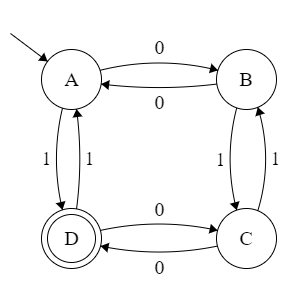
\includegraphics[width=0.4\linewidth]{02/2_1.png}

Proof:

Let's look at what the states mean:

\begin{itemize}
    \item A: State $A$ represents words that contain an even number of $0$'s and $1$'s.
    \item B: State $B$ represents words that contain an odd number of $0$'s and an even number of $1$'s.
    \item C: State $C$ represents words that contain an odd number of $0$'s and an odd number of $1$'s.
    \item D: State $D$ represents words that contain an even number of $0$'s and an odd number of $1$'s.
\end{itemize}

Let's look at the starting state and the accepting and rejecting states:

\begin{itemize}
    \item The starting state is the state that should represent the empty string. The empty string contains zero $0$'s and zero $1$'s, and zero is even, which is represented by $A$, so the starting state is $A$.
    \item The only accepting state is $D$, since we want to accept words that contain an even number of zeros and an odd number of ones, which are represented by $D$.
    \item $A$,$B$ and $C$ are rejecting states, since they represent words that are not in the desired language.
\end{itemize}

Let's look at the transitions:

\begin{itemize}
    \item Transitions triggered by a $0$ input are $A\rightarrow{}B$, $B\rightarrow{}A$, $C\rightarrow{}D$, $D\rightarrow{}C$. In these cases the parity of the $1$'s doesn't change, while the parity of the $0$'s is inverted. If we look back on what the states represent we can verify in all $4$ cases that this is the case.
    \item Transitions triggered by a $1$ input are $A\rightarrow{}D$, $D\rightarrow{}A$, $B\rightarrow{}C$, $C\rightarrow{}D$. In these cases the parity of the $0$'s doesn't change, while the parity of the $1$'s is inverted. If we look back on what the states represent we can verify in all $4$ cases that this is the case.
\end{itemize}\pagebreak
\subsection{Session 2, Exercise 2}

\lineparagraph{Exercise}

Let $\Sigma=\{0,1\}$. Give a deterministic finite automaton that accepts the words that contain an even number of zeroes, while the number of ones is divisible by three.

\lineparagraph{Solution}


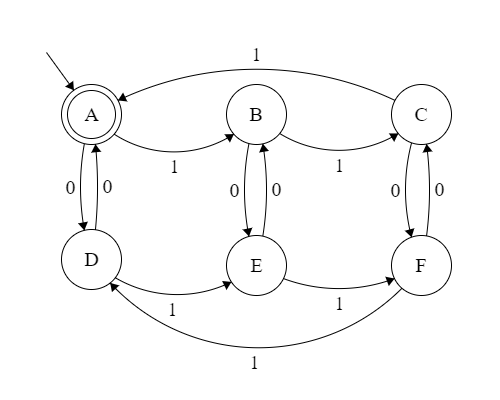
\includegraphics[width=0.5\linewidth]{02/2_2.png}

Proof:

Let's look at what the states mean:

\begin{itemize}
    \item A: State $A$ represents words that contain an even number of $0$'s and the number of $1$'s is in the form $3k$ (divisible by three).
    \item B: State $B$ represents words that contain an even number of $0$'s and the number of $1$'s is in the form $3k+1$.
    \item C: State $C$ represents words that contain an even number of $0$'s and the number of $1$'s is in the form $3k+2$.
    \item D: State $D$ represents words that contain an odd number of $0$'s and the number of $1$'s is in the form $3k$ (divisible by three).
    \item E: State $E$ represents words that contain an odd number of $0$'s and the number of $1$'s is in the form $3k+1$.
    \item F: State $F$ represents words that contain an odd number of $0$'s and the number of $1$'s is in the form $3k+2$.
\end{itemize}

Let's look at the starting state and the accepting and rejecting states:

\begin{itemize}
    \item The starting state is the state that should represent the empty string. The empty string contains zero $0$'s and zero $1$'s, and zero is even and also divisible by three, which is represented by $A$, so the starting state is $A$.
    \item The only accepting state is $A$, since we want to accept words that contain an even number of zeros and the number of ones is divisible by three in them, which are represented by $A$.
    \item The other states are rejecting states, since they represent words that are not in the desired language.
\end{itemize}

Let's look at the transitions:

\begin{itemize}
    \item Transitions triggered by a $0$ input are $A\rightarrow{}D$, $D\rightarrow{}A$, $B\rightarrow{}E$, $E\rightarrow{}B$, $C\rightarrow{}F$, $F\rightarrow{}C$. In these cases the parity of the $1$'s doesn't change, while the parity of the $0$'s is inverted. If we look back on what the states represent we can verify in all $6$ cases that this is the case.
    \item Transitions triggered by a $1$ input:
    \begin{itemize}
        \item $A\rightarrow{}B$ and $D\rightarrow{}E$ move from states that have seen $3k$ $1$'s to states that have sen $3k+1$ $1$'s (the remainder goes from $0$ to $1$).
        \item $B\rightarrow{}C$ and $E\rightarrow{}F$ move from states that have seen $3k+1$ $1$'s to states that have sen $3k+2$ $1$'s (the remainder goes from $1$ to $2$).
        \item $C\rightarrow{}A$ and $F\rightarrow{}D$ move from states that have seen $3k+2$ $1$'s to states that have sen $3k$ $1$'s (the remainder goes from $2$ to $0$).
    \end{itemize}
\end{itemize}\pagebreak
\subsection{Session 2, Exercise 03}

\lineparagraph{Exercise}

Let $\Sigma=\{0,1\}$. Give a deterministic finite automaton that accepts the words that contain at least three $1$'s.

\lineparagraph{Solution}
\pagebreak
\subsection{Session 2, Exercise 04}

\lineparagraph{Exercise}

Let $\Sigma=\{0,1\}$. Give a deterministic finite automaton that accepts the words that do not contain the subword $001$.

\lineparagraph{Solution}

When dealing with \textbf{deterministic} finite automatons, a useful trick to keep in mind: sometimes it is easier to give a DFA for the complementer of the language, and then a DFA for the original language can be quickly created.

IMPORTANT: This trick only works for \textbf{deterministic finite automatons}!!!

\textbf{Step 1}: Create DFA for the complementer of the language:

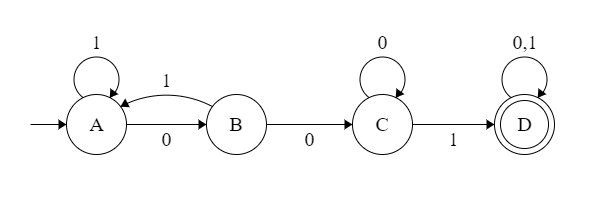
\includegraphics[width=0.6\linewidth]{02/2_4.png}

\textbf{Step 2}: Invert the accept/reject status of the states:

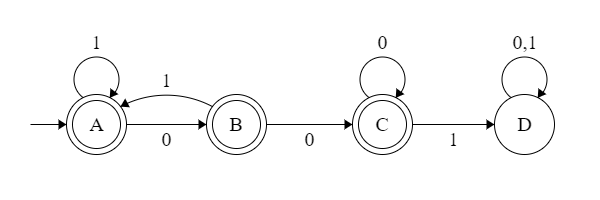
\includegraphics[width=0.6\linewidth]{02/2_4_inv.png}

Proof:

Let's look at what the states mean:

\begin{itemize}
    \item A: State $A$ represents words that end in something that is not a prefix of $001$: they either are the empty string or they end in a $1$; and do not contain $001$ itself.
    \item B: State $B$ represents words that end in $0$.
    \item C: State $C$ represents words that end in $00$.
    \item D: State $D$ represents words that contain $001$.
\end{itemize}

Let's look at the starting state and the accepting and rejecting states:

\begin{itemize}
    \item The starting state is the state that should represent the empty string. The empty string contains no prefix of $001$, so it is represented by $A$.
    \item In the original DFA words that contain $001$ were accepted, which is represented by state $D$, while states $A$,$B$ and $C$ were rejecting.
    \item To get a DFA for the complementer of the language, we simply need to accepts words that we have rejected before and reject words that we have accepted before. This is done by making states $A$,$B$ and $C$ accept, while making state $D$ reject.
\end{itemize}

Let's look at the transitions:

\begin{itemize}
    \item In state $A$, when we read in a $0$ we can move to state $B$, since now the current ending is $0$. However when we read $1$'s, we are not getting closer to finding a $001$ substring (we need the $0$'s first), so we just discard them.
    \item In state $B$, we have the ending $0$. When we read another $0$ in, this results in having the ending $00$, so we can move forward to state $C$, one step closer to finding the substring $001$. However if we read in a $1$, this ruins our progress, since the current ending is now $01$, but we needed a $00$. We can't even stay in state $B$, since we would need a $0$ ending for that, but the last character has been a $1$. We have to move all the way back to state $A$.
    \item In state $C$ the current ending is $00$. If we read in a $1$, that means we just found a $001$ substring, we can move to state $D$! And if we read a $0$ in, while we can't move to state $D$, we can stay in $C$, since the current ending is $000$, or discarding the oldest $0$: $00$, which means we can stay in state $C$.
    \item In state $D$ we have already found the substring, we just read in the remainder of the input, discard it and accept when done.
\end{itemize}\pagebreak
\subsection{Session 2, Exercise 05}

\lineparagraph{Exercise}

Which words are accepted by this automaton? ($\Sigma=\{0,1\}$).

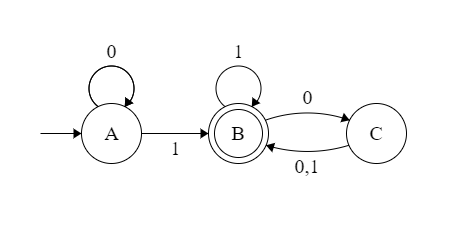
\includegraphics[width=0.5\linewidth]{02/2_5_automaton.png}

\lineparagraph{Solution}
\pagebreak
\subsection{Session 2, Exercise 6}

\lineparagraph{Exercise}

Perform the following for both nondeterministic finite automata.
\begin{enumerate}[a.)]
    \item Give the computation tree of word $baabab$.
    \item Create an equivalent DFA by the procedure studied in class.
    \item Which languages are recognized by these automata?
\end{enumerate}

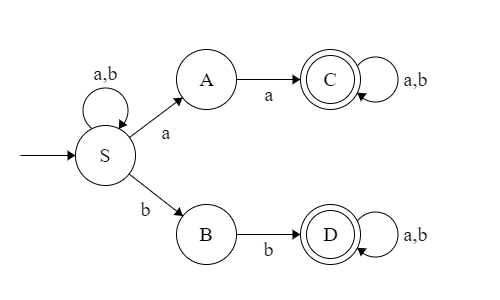
\includegraphics[width=0.5\linewidth]{02/2_6_1_automaton.png}

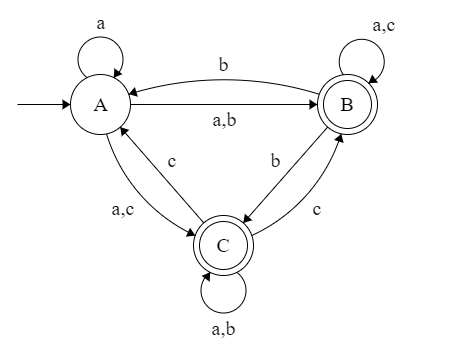
\includegraphics[width=0.5\linewidth]{02/2_6_2_automaton.png}

\lineparagraph{Solution}

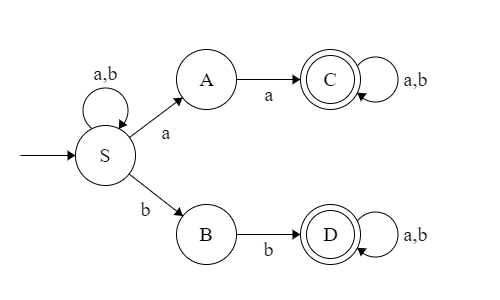
\includegraphics[width=0.5\linewidth]{02/2_6_1_automaton.png}

Give the computation tree of word $baabab$:

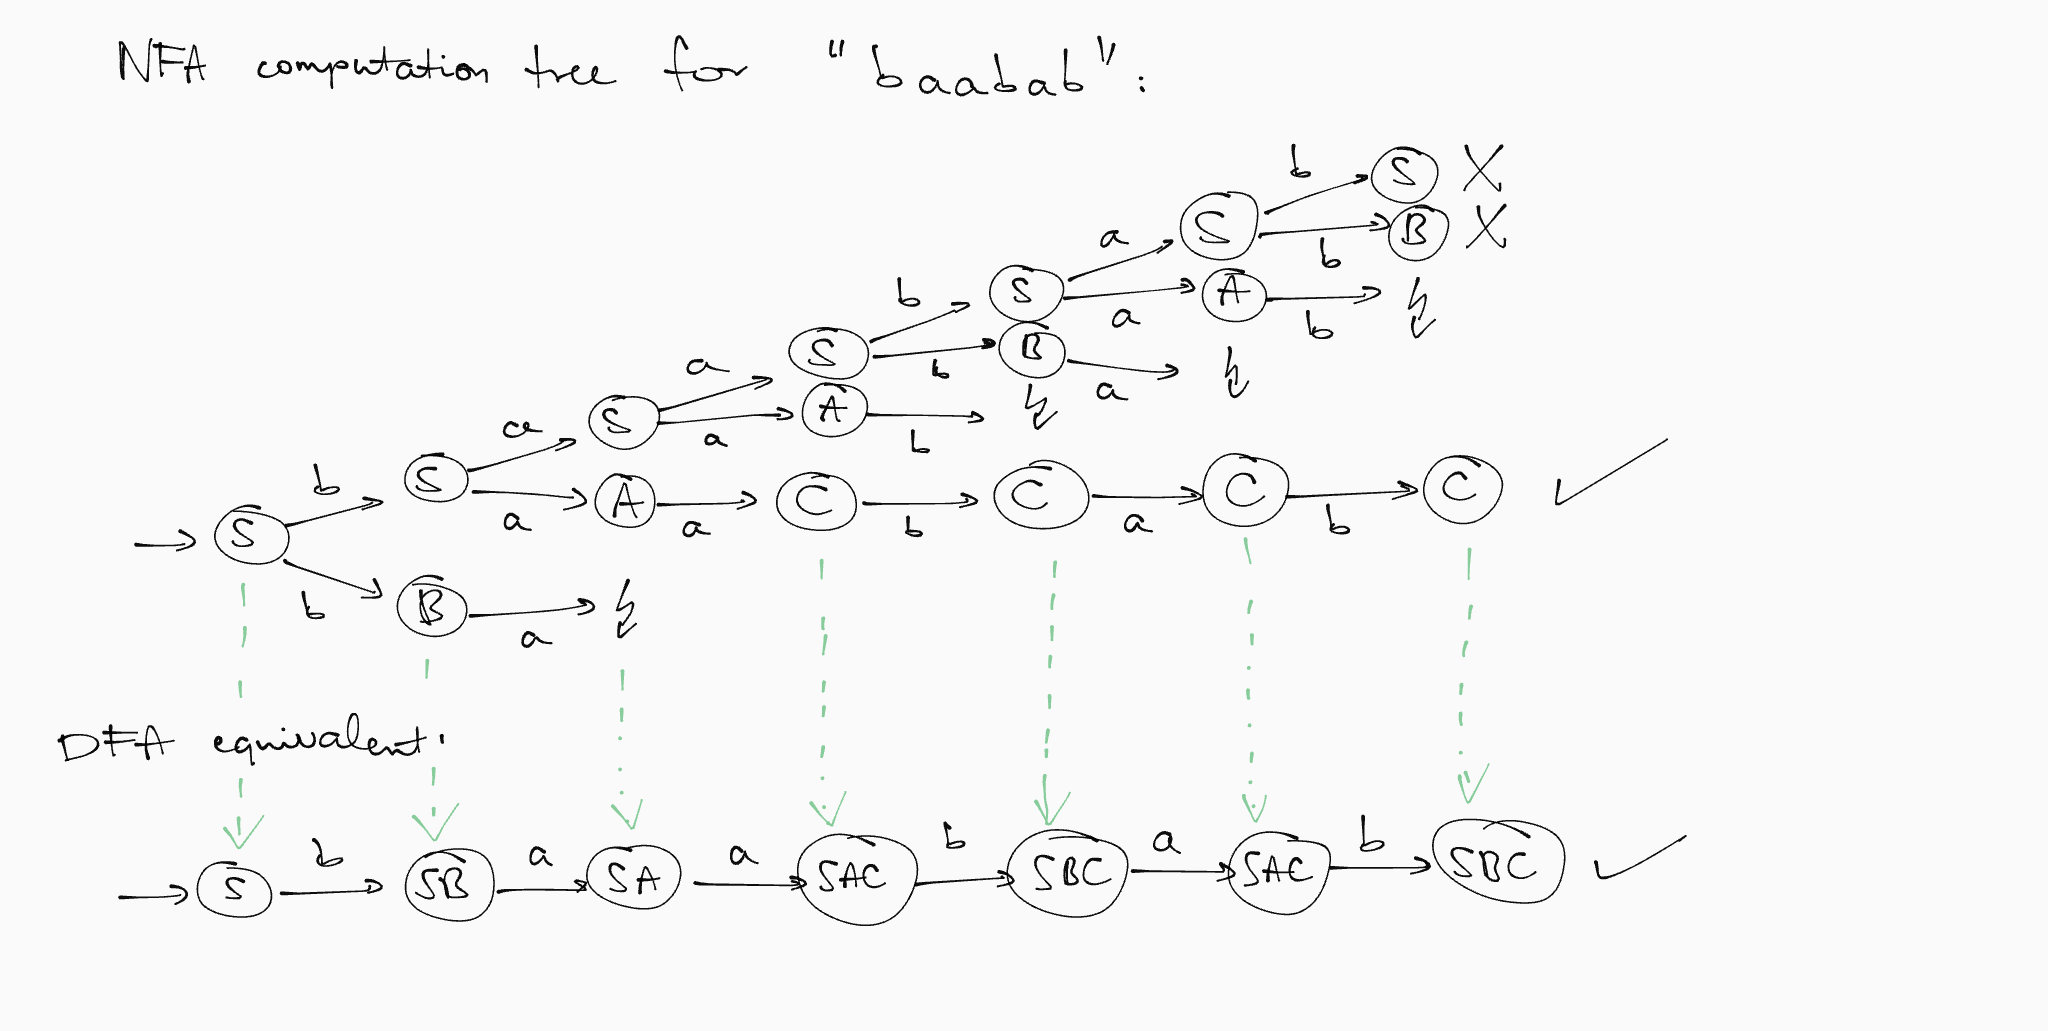
\includegraphics[width=\linewidth]{02/comp_tree_1_nfa_dfa.png}

The word $baabab$ is accepted, since there exists a branch that resulted in an accept state ($C$).

The DFA equivalent computation is also shown in the drawing. We basically follow all branches in ''parallel'', using meta states. We will construct the DFA, that will do a computation like this one:

\textbf{Step 1}

We start with the same starting state as in the NFA: $S$.

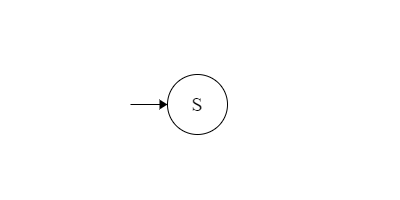
\includegraphics[width=0.5\linewidth]{02/dfa_step_01.png}

\textbf{Step 2}

Then, we check where can we move for an $a$ input from $S$ in the NFA: $S\xrightarrow{a}\{S,A\}$, so we add the $SA$ state for an $a$ transition, and similarly for $S\xrightarrow{b}\{S,B\}$, so we add the $SB$ state for a $b$ transition.

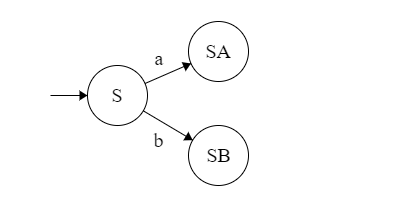
\includegraphics[width=0.5\linewidth]{02/dfa_step_02.png}

Check back on the DFA equivalent on the drawing above! You will notice the state $SB$ as the second step.

\textbf{Step 3}

And we continue the same thing for the new states:

Where does $SA$ move for an input character of $a$? The transitions from $S$ and from $A$ for input $a$ are: $S\xrightarrow{a}\{S,A\}$ and $A\xrightarrow{a}\{C\}$, so together they move to state $SAC$.

Where does $SA$ move for an input character of $b$? The transitions from $S$ and from $A$ for input $b$ are: $S\xrightarrow{b}\{S,B\}$ and $A\xrightarrow{b}\{\}$, so together they move to state $SB$.

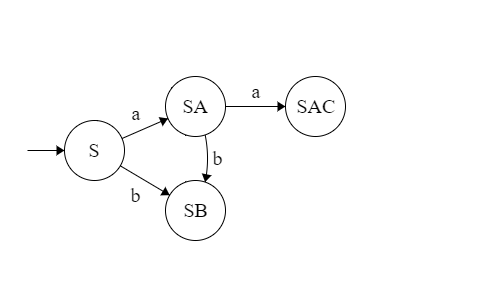
\includegraphics[width=0.7\linewidth]{02/dfa_step_03.png}

The process is the same: find a state that does not have all transitions defined (for $a$ and for $b$ input as well), check where their basis states transition in the NFA for the given input and add it as a transition. If the resulting state does not exist, add the state.

When no new states are added and all states transitions are fully defined the process is done.

\textbf{Step 4}

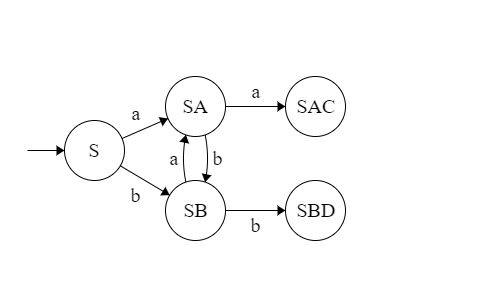
\includegraphics[width=0.7\linewidth]{02/dfa_step_04.png}

\textbf{Step 5}

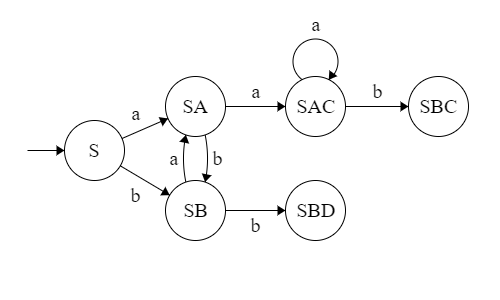
\includegraphics[width=0.7\linewidth]{02/dfa_step_05.png}

\textbf{Step 6}

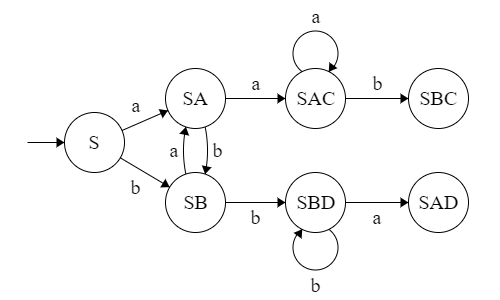
\includegraphics[width=0.7\linewidth]{02/dfa_step_06.png}

\textbf{Step 7}

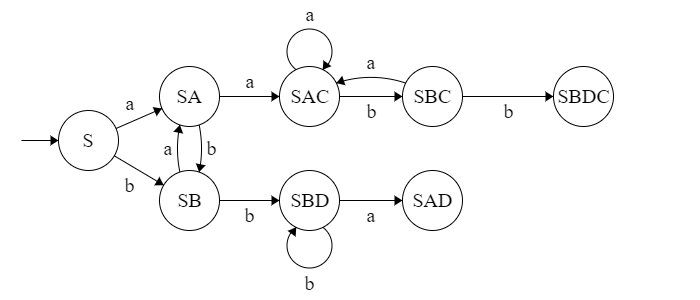
\includegraphics[width=0.9\linewidth]{02/dfa_step_07.png}

\textbf{Step 8}

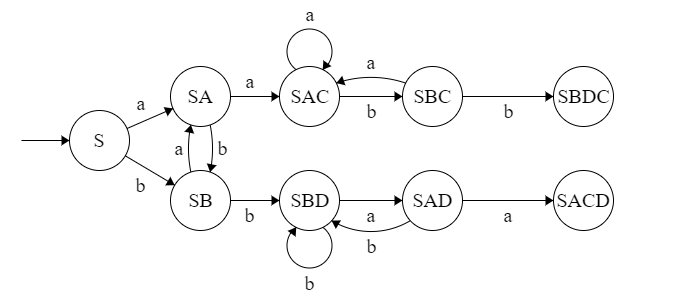
\includegraphics[width=0.9\linewidth]{02/dfa_step_08.png}

\textbf{Step 9}

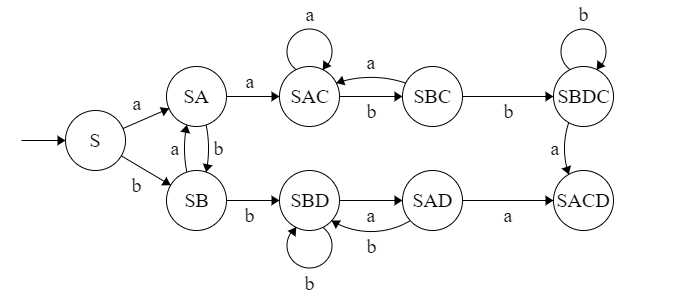
\includegraphics[width=0.9\linewidth]{02/dfa_step_09.png}

\textbf{Step 10}

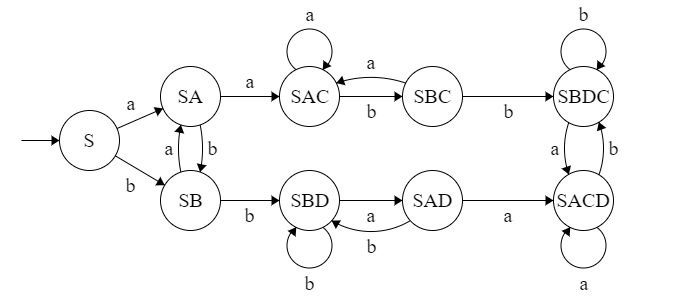
\includegraphics[width=0.9\linewidth]{02/dfa_step_10.png}

\textbf{Step 11}

Finally, define the accepts states: Any state that contains an original accept state (in this case $C$ or $D$) will be an accepting state:

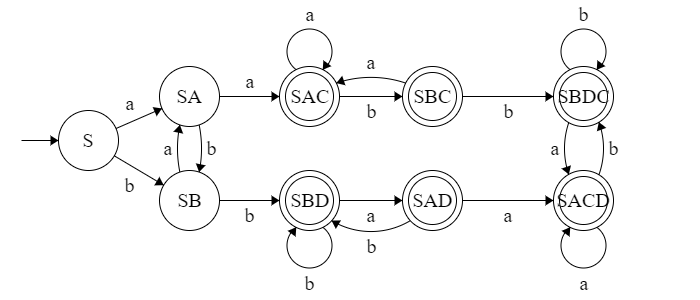
\includegraphics[width=0.9\linewidth]{02/dfa_step_11.png}

\textbf{Note}

By the way, the automaton can be simplified, like this:

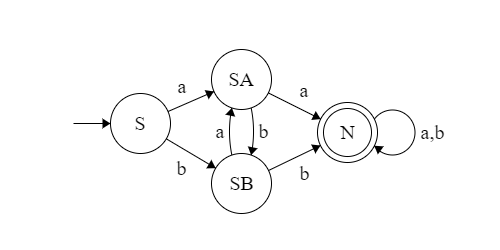
\includegraphics[width=0.7\linewidth]{02/dfa_final.png}

Since the moment we reach any of the accepts states, we will never leave them.


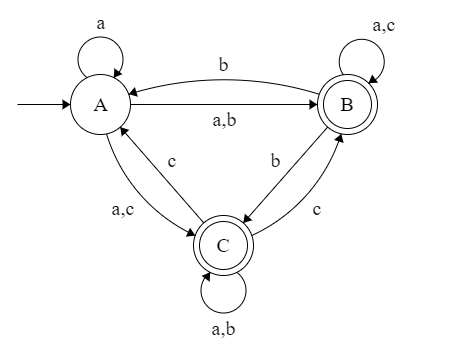
\includegraphics[width=0.5\linewidth]{02/2_6_2_automaton.png}

TODO\pagebreak
\subsection{Session 2, Exercise 7}

\lineparagraph{Exercise}

Give a nondeterministic finite automaton that accepts those words that have 10100 as subword.

\lineparagraph{Solution}

The key to solving this exercise using a nondetermnistic automaton is to create a delayed start on the starting state by introducing a 0,1 loop on it:

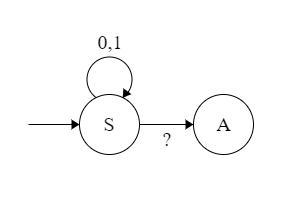
\includegraphics[width=200px]{02/wait_to_start.png}

This will "eat up" some prefix of the input word before allowing the computation to proceed to state A. Whatever we put in place of the ? on the leaving transition will be a nondeterministic choice for the automaton.

The next step is to add the success path to the automaton which contains the string we want to have as a subword: 10100.

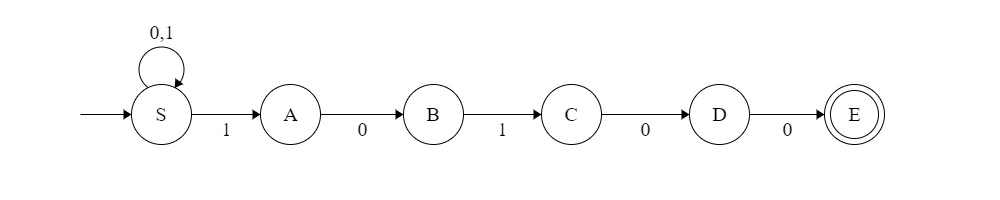
\includegraphics[width=\linewidth]{02/success_path.png}

Then finally, let's allow "eating up" any remaining suffix of the word as well:

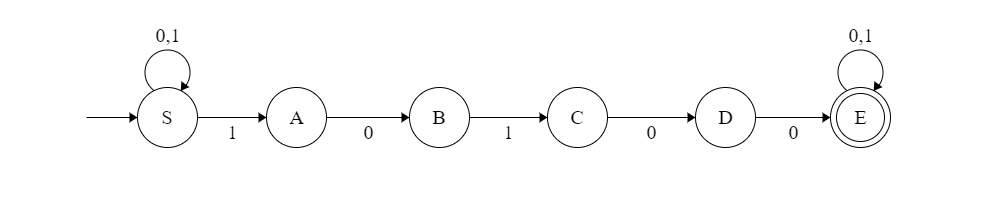
\includegraphics[width=\linewidth]{02/10100.png}

Some observations:

\begin{itemize}
    \item Firstly, this is a nondeterministic finite automaton: Notice how in state $S$, for an input character of $1$ we can either remain in $S$, or move to state $A$.
    \item There are also transitions missing: it is an incomplete finite automaton as well. For example, in state $A$, for an input character of 1, the machine halts (and halting due to a missing transition means rejection, \textbf{regardless of the current state's accept/reject status}.
    \item Notice how visually similar this automaton is to the regular expression for the same language: $(0+1)^*10100(0+1)^*$.
\end{itemize}

Let's look at an example computation on the word 1110100, which is in the language of the automaton.

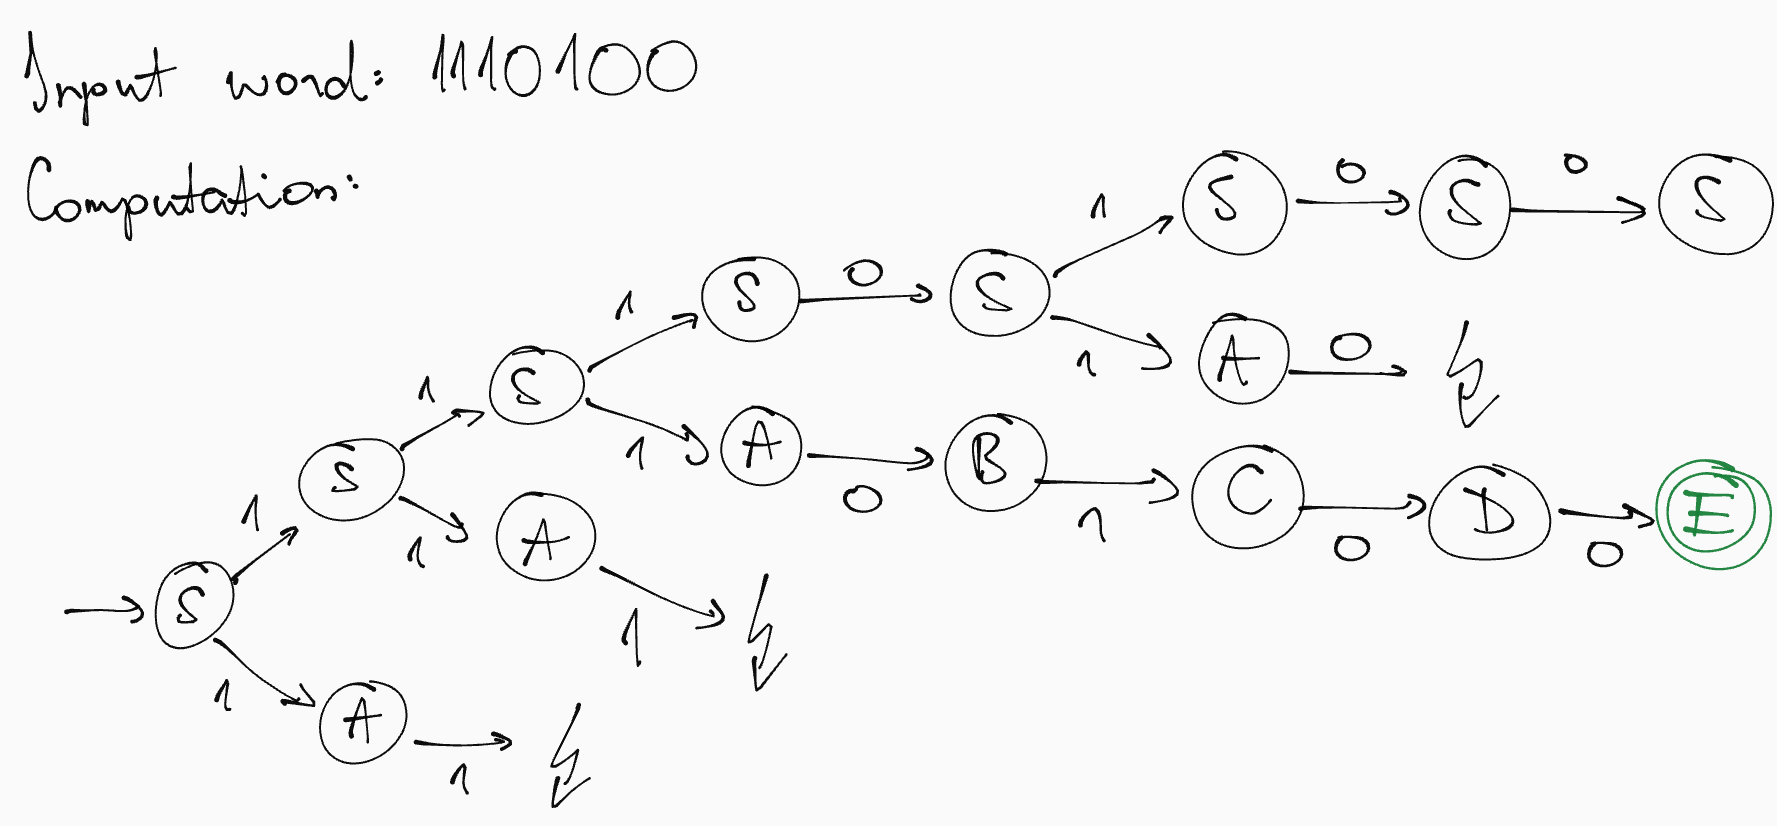
\includegraphics[width=\linewidth]{02/computation_1110100.png}

\begin{itemize}
    \item See, how it tried to leave state $S$ and move to state $A$ many times in different places of the input string? Many times it failed, when the timing was incorrect. Maybe it was too early, when the first two 1's, which are not part of the matching subword were given to it, or it was too late, when the pattern was already gone.
    \item There was already a lazy case, the top branch, which just remained in state $S$ forever, which also could not succeed.
    \item However there only needs to be a single successful branch and it only needs to time its move to state $A$ correctly once: on the third branch it successfully finished in state $E$, which means that the word is accepted, correctly!
    \item Notice how it is only possible to reach state $E$, when the input word contains 10100. We need a 1 to move from $S$ to $A$, then we need a consecutive $0$ to move from $A$ to $B$, then we need a consecutive $1$ to move from $B$ to $C$, then we need a consecutive $0$ to move from $C$ to $D$, then we need another consecutive $0$, to move from $D$ to $E$.
    \item When the timing is just right and we catch the beginning of the pattern we can ''sail smoothly'' towards $E$.
\end{itemize}

When you are on the exam, you will need to give some sort of proof that the automaton you wrote up does what the exercise is asking you to do. For this exercise this is how a proof like this might look like:

\textbf{Proof:}

1. Let's look at the states of the automaton:
What the different states mean and why their transitions are correct.
\begin{itemize}
    \item State $S$ is the starting state. Here, we non-deterministically wait to start our computation, using the $0$,$1$ loop. Since the first character of the pattern we seek is a $1$, on an input character of $1$, the automaton can decide to move to state $A$.
    \item State $A$ represents the information "already read the first character of the pattern". Here, we allow a transition to state $B$ if the second character of the pattern comes, which is a $0$. However, the transition for an input of $1$ is missing, which means that the computation (on that branch) will halt. This is correct, because the pattern's characters must be consecutive.
    \item States $B$, $C$ and $D$ work similaly: they represent the next character recognized from the pattern we seek and we only allow a transition for the upcoming character from the pattern to move forward, towards $E$.
    \item Finally, state $E$ represents "pattern found". This means that we can accept the word, furthermore, any further input characters are allowed, since the pattern can be anywhere in the word.
\end{itemize}

2. Let's look at the accepted and rejected words of the automaton:

Any word that contains the pattern 10100 will be accepted, because the automaton on the (single) accepting branch of the computation first non-deterministically reads the prefix of the word before the pattern, then transitions from $S$, to $E$ using the consecutive characters of the pattern, then finally in state $E$ further characters can be read (the remaining suffix of the word) and the word will be accepted.

Any word that does not contain the pattern 10100 can not reach state $E$, because each step towards $E$ requires the next character of the pattern to be present consecutively in the word. There is correct timing to leave $S$, no computational branch can end up in $E$, so the word will be rejected.

\textbf{(End of proof.)}

(Due to time limits on the exam, it is okay to not use full sentences like I did above, abbreviate things, etc.)

It is important when doing these proofs, that you do not use a specific input word as an example, but generalize to any possible words, like the proof above.

\lineparagraph{Deterministic solution}

This exercise allows us to truly appreciate nondeterministic automata, since it made it really easy for us to come up with a design for a given subword.

However, the task is also possible with a deterministic automaton (it must be, since we can convert any NFA into a DFA, but there is an even easier method to obtain a DFA, than the general conversion algorithm). This is not part of the task, but nice to see how it works as well.

Step 1: Get rid of loop on the starting state, we need to be deterministic now.

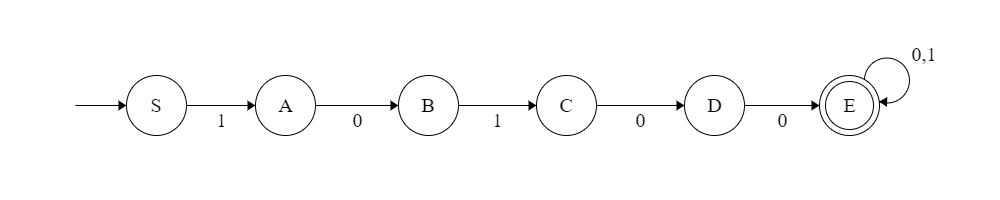
\includegraphics[width=\linewidth]{02/det_10100_1.png}

Step 2: Put in the missing transitions, states $S$-$D$ all miss 1 of them.

The main idea here is that the missing transitions are failures in recognizing the next character of the pattern at the current position. How big of a failure it is depends on what the pattern we have found so far is and how much of it can be salvaged when we add the incorrect character at the end.

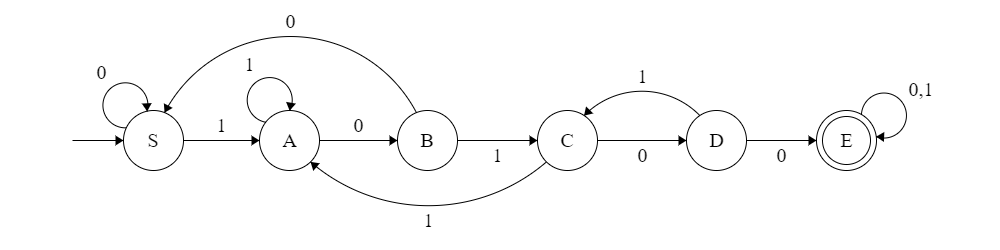
\includegraphics[width=\linewidth]{02/det_10100_2.png}

\begin{itemize}
    \item When we are in state $S$, the pattern we have found so far is nothing. Until we read $0$'s we remain in state $S$, since the first character of the pattern is a $1$.
    \item When we are in state $A$, the pattern we have found so far is ''$1$''. If we read another $1$ now, we now have ''$11$''. The pattern is ''$10100$'', so that second $1$ character can still turn out to be the beginning of the pattern, so we need to remember that we have a ''$1$'' and thus stay in state $A$.
    \item When we are in state $B$, the pattern we have found so far is ''$10$'', if we read a $0$ in now, that makes it a ''$100$''. Unfortunately, there is no salvaging this: not ''$100$'', not ''$00$'' and not even a single ''$0$'' is useful for us, neither of them are the prefixes of the pattern ''$10100$''. We need to scratch everything and go back to state $S$.
    \item When we are in state $C$, the pattern we have found so far is ''$101$''. If we read a $1$ now, that makes it ''$1011$''. The possible suffixes to remember here are ''$011$'', ''$11$'' and ''$1$''. In general we always need to keep the longest one that is still a prefix of the pattern: in this case, that is ''$1$'', which is represented by state $A$, so we move back there.
    \item When we are in state $D$, the pattern we have found so far is ''$1010$''. If we read a $1$ now, that makes it ''$10101$''. This is great news, because we can actually just forget the first two characters and we can still keep the remaining ''$101$'', which is the first three characters of the pattern! Not much is lost, ''$101$'' is represented by state $C$, so we can move there.
\end{itemize}\pagebreak
\subsection{Session 2, Exercise 08}

\lineparagraph{Exercise}

Prove that the language that consists o those words that have two $1$'s such that the number of $0$'s between them is divisible by four, is regular. (There could be several $1$'s between the two chosen $1$'s, besides the $4k$ $0$'s.)

\lineparagraph{Solution}
\pagebreak
\subsection{Session 2, Exercise 09}

\lineparagraph{Exercise}

Design a finite automaton that accepts positive rational numbers written in decimal form. ($\Sigma$ contains the decimal point and digits $0,1,2,3,4,5,6,7,8,9$.) The number to be accepted is either an integer without decimal point (e.g. $123$), or it contains a decimal point. In this latter case numbers without integer part or fractional part must also be accepted, but at most one of these parts may be missing. (For example, $123.456$, $123.$ and $.456$ are all accepted, but a single decimal point is not.) It is also requested that a number cannot begin with dummy $0$'s, however $0.456$ is OK.)

\lineparagraph{Solution}
\pagebreak
\subsection{Session 2, Exercise 10}

\lineparagraph{Exercise}

Let $\Sigma = \{0, 1\}$. The sequences are considered as binary numbers. Give a finite automaton that accepts exactly those words that represent numbers divisible by three in binary form. Take into consideration that a number does not begin with $0$, except for number zero itself, and that the input number is read beginning with the most significant digit.

\lineparagraph{Solution}

Any automaton that we design will work by reading the input binary string from left to right. We will want to keep track of the remainder of the current binary number after each 0 or 1 we read. The question is how do we update this remainder when the next input character comes? First, let's do a simpler task, just keeping track of the number itself and updating it as we go.

\begin{itemize}
    \item For example, let's say that so far we have read the the ''$101$'' binary string on the input. That is a $5$ in decimal form.
    \item Let's say the next character is also a $1$, so now the current string is ''$1011$'', or in decimal form $11$.
    \item This was achieved by shifting the string ''$101$'' to the left and adding a ''$1$'' as the least significant character.
    \item A left shift in binary corresponds to multiplication by $2$ in decimal, and then if the next character is a $1$, we just need to add $1$ to the decimal value as well. So in our example, $5*2 + 1 = 11$.
    \item In general, if we read a binary number from left to right, to calculate its decimal value, we simply multiply the current decimal value by $2$, and if the bit we read was a $1$, we add a $1$ and continue to the next bit.
\end{itemize}
 
If we don't care about the entire number, just its remainder when divided by $3$, we can do the same calculation, but modulo $3$.

If the current number is divisible by $3$, or in the form $3k$, and the next binary character is a $0$, then to update we do $3k*2+0 = 6k$, which means that the updated number will still be divisible by $3$.

If the next binary character is a $1$, then to update we do $3k*2+1=6k+1=3*(2k)+1$, which means that the updated number has a remainder of $1$ when divided by $3$.

We can represent these statements by the following two transitions from state $3k$:

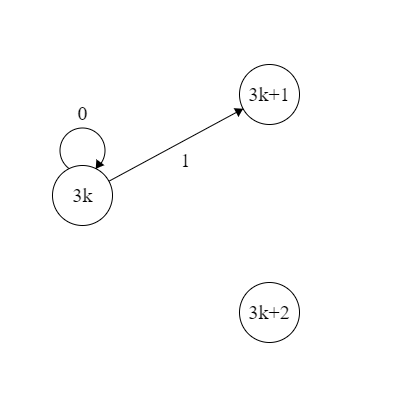
\includegraphics[width=250px]{02/modulo_1.png}

If the current number has a remainder of $1$, when divided by $3$, or in the form of $3k+1$, and the next binary character is a $0$, then to update we do $(3k+1)*2+0=6k+2=3*(2k)+2$, which means that the updated number has a remainder of $2$, when divided by $3$.

If the next binary character is a $1$, then to update we do $(3k+1)*2+1=6k+3=3*(2k+1)$, which means that the updated number is divisible by $3$.

We can represent these statements by the additional two transitions from state $3k+1$:

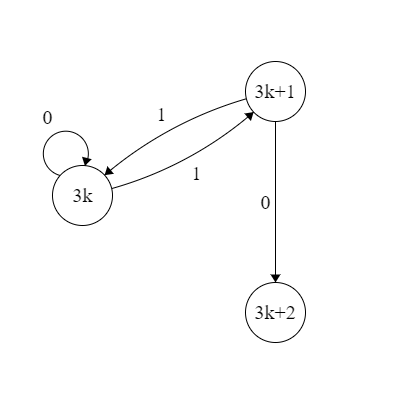
\includegraphics[width=250px]{02/modulo_2.png}

Finally, if the current number has a remainder of $2$, when divided by $3$, or in the for of $3k+2$, and the next binary character is a $0$, then to update we do $(3k+2)*2+0=6k+4=3*(2k+1)+1$, which means that the updated number has a remainder of $1$, when divided by $3$.

If the next binary character is a $1$, then to update we do $(3k+2)*2+1=6k+5=3*(2k+1)+2$, which means that the updated number has a remainder of $2$, when divided by $3$.

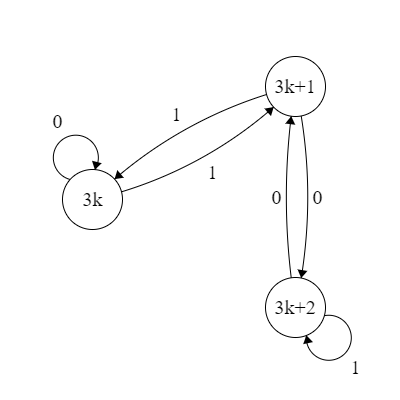
\includegraphics[width=250px]{02/modulo_3.png}

If you want to try this automaton, come up with any decimal number, turn it into binary form and calculate its remainder by $3$, by applying the transitions above using its binary form as input. The starting state should be $3k$, since when we have not read anything in yet, so we want to start from a state that is equivalent to the number $0$, which is divisible by $3$.

I however, did not mark a starting state yet on this image, because there is one additional statement to keep in mind: ''Take into consideration that
a number does not begin with $0$, except for number zero itself.''. This means that we do not consider any string longer than 1 characters starting with a $0$ a number, much less a number that is divisible by $3$, so we need to reject these words.

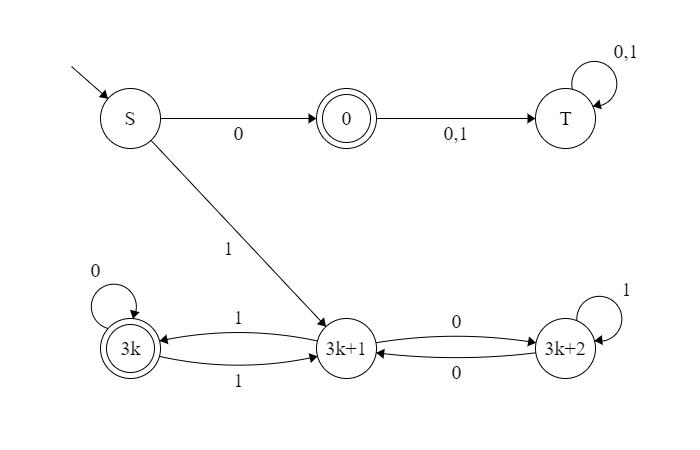
\includegraphics[width=\linewidth]{02/modulo_final.png}

Now, if this was an exam, here is how to prove that this accepts the language: (Basically everything I just said, but in a shortened form.)

\textbf{Proof:}

1. Let's explain what the different states mean and that their transitions are correct:

\begin{itemize}
    \item $S$ is the starting state. If we read a $0$ in, we move to a state dedicated to the number $0$. If we read a $1$ in, we move to the state that represents binary numbers, that give a remainder of $1$ when divided by $3$, which is true for the (binary) number $1$.
    \item The only word for state $0$ is $0$ itself, this is divisible by $3$ and is accepted. If we read anything else after a $0$ that is an incorrectly formatted number and moves to a trap state $T$ which rejects it.
    \item The states $3k$, $3k+1$ and $3k+2$ represent the 3 remainder classes of division by $3$. When a new character is read on the input, we update the remainder class with multiplying by $2$ (binary shift) and adding the $0$ or $1$ bit we just read. We can see that the transitions are correct, since:
    \begin{itemize}
        \item $3k*2+0 = 3*(2k)$
        \item $3k*2+1 = 3*(2k)+1$
        \item $(3k+1)*2+0 = 3*(2k)+2$
        \item $(3k+1)*2+1 = 3*(2k+1)$
        \item $(3k+2)*2+0 = 3*(2k+1)+1$
        \item $(3k+2)*2+1 = 3*(2k+1)+2$
    \end{itemize}
\end{itemize}

2. Let's explain that the correct words are accepted and the words not in the language are rejected:

The words in the language are any numbers that are divisible by $3$, which is either the number $0$ or anything that is in the form $3k$, these states are accepting.

A word could be outside of the language due to being malformed (starting with $0$, but not being $0$ itself), which will be redirected to a trap $T$; or due to not being divisible by $3$, in which case it will land in either $3k+1$ or $3k+2$ and will be rejected there. Finally, the empty string is rejected because it's not a number, which is the only word that will end up in state $S$.

\textbf{(End of proof.)}

Notes:

\begin{itemize}
    \item I ended up making a deterministic automaton here, however the task would allow a non-deterministic one as well. We could get rid of the enitre $T$ state and define no transitions outwards from state $0$. If there is input left to be read in state $0$ the automaton halts due to a missing transition, which rejects the word regardless of the accept/reject status of the current state!
\end{itemize}\pagebreak
\subsection{Session 2, Exercise 11}

\lineparagraph{Exercise}

Let language $L_k$ consist of those word over alphabet $\Sigma=\{a,b\}$ that have character $b$ on the $k^{\text{th}}$ position counting rom backwards. (For example $bbaa\in{}L_3\cap{}L_4$.)

\begin{enumerate}[a.)]
    \item Prove that there exists a nondeterministic automaton of $k+1$ states recognizing language $L_k$ for all $k\geq{}1$.
    \item Prove that every deterministic automaton recognizing $L_k$ has at least $2^k$ states.
\end{enumerate}

\lineparagraph{Solution}
\pagebreak
\subsection{Session 2, Exercise 12}

\lineparagraph{Exercise}

Prove that every NFA can be transformed so that it recognizes the same language, however it has a unique accept state.

\lineparagraph{Solution}
\pagebreak
\subsection{Session 2, Exercise 13}

\lineparagraph{Exercise}

The language $L^R$ is obtained from language $L$ so that every word in $L$ is reversed, that is the characters of the word are written in reverse order. Prove that $L$ is regular $\Leftrightarrow$ $L^R$ is regular.

\lineparagraph{Solution}
\pagebreak

\section{March 2nd (Session 3): Regular expressions, Context-free languages}
\subsection{}
\label{3.1}

\lineparagraph{Exercise}

Let $\Sigma = \{a,b\}$ and let language $L$ consist of words
that contain the same number of $a$'s and $b$'s. Is $L$ regular?

\lineparagraph{Solution}

\textbf{Gut feeling} (This is not yet a proof!)

Not regular.

This language is similar to $a^nb^n$ (studied in the lecture). The
main issue with it will be similar: we would need to remember the difference
of the number of $a$'s and $b$'s we have read in so far and only
accept the word if the difference is $0$ after reading in the entire
word.

For every possible difference, we will need a separate state, however the
difference can be arbitrarily large, while we can only have a finite
number of states using Finite Automata, so it won't be possible
to construct such a machine.

\textbf{Proof}

We will do proof by contradiction:

\begin{itemize}
    \item Let's assume that $L$ is regular.
    \item Then, that means that there exists a Deterministic Finite Automata, that accepts the language $L$.
    \item Let's take one such automata, and name it $M$.
    \item Let's count the number of states in $M$ and name this number $n$.
    \item Now let's list exactly $n+1$ specifically chosen words from the $L$ language: $ab$, $aabb$, $a^3b^3$, $\dots$, $a^{n+1}b^{n+1}$.
    \item Then imagine feeding these $n+1$ words into $M$. For all of them, let $M$ read in the $a$ letters and then stop and take note of which state the word is at the moment, halfway-through the operation.
    \item After reading in $a$, $aa$, $a^3$, $\dots$, $a^{n+1}$, since these are $n+1$ cases, while $M$ only has $n$ states, we can use the \href{https://en.wikipedia.org/wiki/Pigeonhole_principle}{Pigeonhole Principle} and say, that there exists at least two different half-words $a^i$ and $a^j$ $(i\neq{}j)$, for which $M$ arrived at the same state after feeding it these inputs. Let's name this state $S$.
    \item Since $a^ib^i$ is in language $L$, it must be accepted by $M$. This means that when we continue from state $S$ and feed in the $b$'s of the word, the machine must arrive in an accepting state. So there exists a path from state $S$ to an accepting state that is traversed by the input $b^i$.
    \item However, $M$ also arrives in state $S$ when it reads $a^j$. We just noted, that if from $S$ it reads $b^i$ it will arrive in an accept state. If we put these two together, it means that $M$ accepts the word $a^ib^j$, where $i\neq{}j$, which is \textbf{not} in $L$, since it doesn't have the same number of $a$'s and $b$'s.
    \item We stated in the beginning that $M$ is a machine whose language is $L$, however we just found a word that is not in $L$, but accepted by $M$, so this is a contradiction.
\end{itemize}

Notes:

\begin{itemize}
    \item This is symmetric, we could also prove that $M$ accepts $a^ib^j$, for $i\neq{}j$ which is also a contradiction, since that word is also not in $L$.
    \item To put it shortly: the machine cannot distinguish $a^i$ and $a^j$ $(i\neq{}j)$ and since $a^ib^i$ and $a^jb^j$ are accepted, so are $a^ib^j$ and $a^jb^i$, which are not in $L$, which is a contradiction.
    \item Note, that this proof is exactly the same as the proof for language $a^nb^n$ studied in the lecture. This is due to the fact, that these languages are similar, for both of them the issue is keeping track of the number of $a$'s to (eventually or simultaneously) compare them to the number of $b$'s.
    \item It is \textbf{not true}, that ''the proof works because $a^nb^n$ is a subset of $L$''. For example, $a^nb^n$ is also a subset of $\Sigma^*$, which is regular!
\end{itemize}
\pagebreak
\subsection{Session 3, Exercise 2}

\lineparagraph{Exercise}

Let $\Sigma = \{(,)\}$. Prove that the language of properly matched parentheses sequences is not regular.

\lineparagraph{Solution}

Quite similar to \ref{3f1}. The $n+1$ words from $L$, the language of properly matched parentheses to be used are $()$, $(())$, $(^3)^3$, $\dots$, $(^{(n+1)})^{(n+1)}$, so just substitute $a = ($ and $b = )$.\pagebreak
\subsection{Session 3, Exercise 3}

\lineparagraph{Exercise}

Is the language regular, that consists of sequences of $0$'s of a length that is...
\begin{enumerate}[a.)]
\item an even number?
\item an odd number?
\item a perfect square?
\item a power of $2$?
\end{enumerate}

\lineparagraph{Solution}

\subsubsection{Even number of $0$'s}

Regular.

\textbf{Proof 1}: The regular expression $(00)^*$ matches them.

Proof that this regular expression matches the language:

\begin{itemize}
    \item The $^*$ operator allows any number of repeats, even 0.
    \item Inside the $^*$ operator we have two $0$'s, which can be repeated any number of times to match any even number of $0$'s.
    \item The empty string, also known as zero number of $0$'s contains an even number of $0$'s, so it is part of the language. $(00)^*$ matches the empty string, which is correct.
\end{itemize}

\textbf{Proof 2}: The following DFA accepts the language:

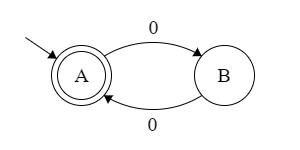
\includegraphics[width=150px]{03/even_zeroes.png}

Proof that this automaton accepts the language:

\begin{itemize}
    \item Words that end up in state $A$ are the words that contain an even number of $0$'s, while words that end up in state $B$ contain an odd number of $0$'s.
    \item The empty string is correctly accepted.
    \item From state $A$, reading another $0$ moves to state $B$, so after reading an even number of $0$'s, if we read one more, now we have an odd number of $0$'s.
    \item And similarly for state $B$.
\end{itemize}

\subsubsection{Odd number of $0$'s}

Regular.

\textbf{Proof 1}: The regular expression $0(00)^*$ matches them.

Proof that this regular expression matches the language:

\begin{itemize}
    \item We have just seen that $(00)^*$ matches an even number of $0$'s.
    \item Adding the $0$ at the front will then match an odd number of $0$'s.
\end{itemize}

\textbf{Proof 2}: The following DFA accepts the language:

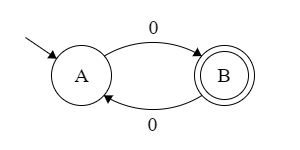
\includegraphics[width=150px]{03/odd_zeroes.png}

Proof that this automaton accepts the language:

\begin{itemize}
    \item This is the same automaton as in the previous exercise, but now the accept state is $B$, to accept an odd number of $0$'s.
\end{itemize}

\subsubsection{A perfect square number of $0$'s}

\textbf{Gut feeling} (This is not yet proof!)

Not regular.

The issue here is going to be, that the length of the accepted words get further and further away from each other as the length of the words increases. We always need to keep track of how far away we are from the next accepted word, how many more $0$'s we need to finally accept. We would need separate states for each of these "$x$ number of $0$'s before we can accept", however $x$ could be arbitrarily large and we only have a finite number of states.

\textbf{Proof}

 Quite similar to \ref{3.1}, the $n+1$ words to use here are of the length of the first $n+1$ square numbers: $0 = 0^{1^2}$, $0000 = 0^{2^2}$, $0^9 = 0^{3^2}$, $0^{16} = 0^{4^2}$, $0^{5^2}$, $0^{6^2}$, $\dots$, $0^{(n+1)^2}$.
 
Then, the finishing of \ref{3.1} is a bit different:

When we find that for an $i\neq{}j$, both $0^{i^2}$ and $0^{j^2}$ end up in the same state $S$, the reasoning is a bit different. Without loss of generality, we can assume that $i<j$. If we were to continue $0^{i^2}$ from state $S$ with $2i+1$ more $0$'s, then the whole input would be $0^{i^2+2i+1} = 0^{(i+1)^2}$, which means that we should accept this word, so from state $S$, for $2i+1$ number of $0$'s we must reach an accept state.

However, this also means that when we continue $0^{j^2}$ (which remember, also arrives in $S$) with $2i+1$ $0$'s, so the word is $0^{j^2+2i+1}$, we will also arrive at the same accept state.

However $j^2+2i+1$ is not a square number. It is between two consecutive square numbers $j^2$ and $(j+1)^2 = j^2+2j+1$, but not equal to either of them:
\begin{itemize}
    \item $j^2 < j^2 + 2i + 1$, since $0<i$.
    \item $j^2 + 2i + 1 < j^2 + 2j + 1$, since $i<j$.
\end{itemize}

Thus, we found a word accepted by $M$, however not in $L$, which is a contradiction.

\subsubsection{A power of $2$}

\textbf{Gut feeling} (This is not yet proof!)

Not regular, the situation is even worse than for square numbers, since powers of $2$ are even further spaced apart as the exponent continues to grow.

\textbf{Proof}

The $n+1$ words to be used are $0^{2^1}$, $0^{2^2}$, $0^{2^3}$, $\dots$, $0^{2^{n+1}}$.

Then similarly to the previous proof, when for $i\neq{}j$, $0^{2^i}$ and $0^{2^j}$ end up in the same state $S$, if we continue by $2^i$ more $0$'s, we should accept, since $0^{2\cdot{}2^i}$ is also a power of two number of $0$'s, however this means  $0^{(2^i + 2^i)}$ will also be accepted, but $2^i + 2^j$ is not a power of $2$, since $i\neq{}j$.\pagebreak
\subsection{Session 3, Exercise 4}

\lineparagraph{Exercise}

Let $\Sigma=\{0,1\}$. Determine the languages of the following regular expressions.

\begin{enumerate}[a.)]
\item $(0+1)^*011(0+1)^*$
\item $1(0+1)^*0$
\item $((0+1)(0+1))^*$
\end{enumerate}

\lineparagraph{Solution}

$(0+1)^*$ is a regular expression that accepts any string from $\Sigma^*$, since $0+1$ accepts either a $0$ or a $1$, and the $^*$ operator allows any number of repeats, including zero.

Thus, $(0+1)^*011(0+1)^*$ is a regular expression that accepts strings that can begin anyhow (including the empty string), then contain the word $011$, then end anyhow, including the empty string. Or, simply put, it accepts all words that contain the string $011$.

For $1(0+1)^*0$, the string must begin with a $1$ and must end with a $0$, while anything, including the empty string can be in between. So this regular expression accepts words that begin with a $1$ and end with a $0$.

For $((0+1)(0+1))^*$, the inner regular expression $(0+1)(0+1)$ accepts any strings with a length of two. Using the $^*$ operator on this allows this to repeat any number of times, allowing for any even length to be accepted, including the length of $0$, which is the empty string.\pagebreak
\subsection{Session 3, Exercise 5}

\lineparagraph{Exercise}

Give regular expressions for the languages over alphabet $\{0,1\}$ that consist of the following words.

\begin{enumerate}[(a)]
\item Words of odd lengths.
\item Words of even length that start and end with $1$.
\item Words containing at least three $0$'s.
\item Words containing an even number of $0$'s.
\item Words of odd lengths starting with $0$ and words of even length starting with $1$.
\item Words of odd length containing subword $00$.
\end{enumerate}

\lineparagraph{Solution}

\subsubsection{Words of odd lengths}

From the previous exercise we know, that $((0+1)(0+1))^*$ accepts the words of even lengths. If we add a $(0+1)$ at the beginning it will add one more character to the lengths, making them odd: $(0+1)((0+1)(0+1))^*$.

\subsubsection{Words of even length that start and end with 1}

To start and end with $1$'s, the regular expression will be $1\text{<something here>}1$. For <something here>, we need to add a regular expression, that together with the two other $1$'s will allow for an even number of characters. So without the two $1$'s, we need an even number of characters, for which we know the regular expression: $((0+1)(0+1))^*$. Putting these together we arrive at $1((0+1)(0+1))^*1$. Since $((0+1)(0+1))^*$ accepts the empty string, the final regular expression will also accept $11$, which is the shortest possible string in the language.

\subsubsection{Words of odd length that start and end with 1}

This was not in the exercise, however I would like to illustrate a point here.

Let's follow the same pattern of thought, as in the previous exercise:
\begin{itemize}
    \item To start and end with $1$'s, the regular expression will be $1\text{<something here>}1$. \item For <something here>, we need to add a regular expression, that together with the two other $1$'s will allow for an odd number of characters.
    \item So without the two $1$'s, we need an odd number of characters, for which we know the regular expression: $(0+1)((0+1)(0+1))^*$.
    \item Putting these together we arrive at $1(0+1)((0+1)(0+1))^*1$.
    \item We have made a mistake...
\end{itemize}

What is the shortest word in this language? It's $1$, which is not accepted by the regular expression above. The issue is that we did not think about the fact, that both starting and ending in a $1$ can also literally mean the same $1$ character, nothing more.

In general, it is always important when building regular expressions from multiple parts, to check for short strings in the language, to see if our expression works for the simplest cases as well.

In this example, to fix the regular expression above, we simply append the missing case at the end: $1(0+1)((0+1)(0+1))^*1 + 1$. This accepts words of length $1$, $3$, and so on, which is what we've wanted.

\subsubsection{Words containing at least three 0's}

Anything can go between the $0$'s, so simply $(0+1)^*0(0+1)^*0(0+1)^*0(0+1)^*$. The three $0$'s between the $(0+1)^*$'s enforce that the string must contain at least three $0$'s.

\subsubsection{Words containing an even number of 0's}

Let's start by words containing exactly two $0$'s: $1^*01^*01^*$. Then, to allow an even number of $0$'s, we can use the $^*$ operator on this: $(1^*01^*01^*)^*$. However, this regular expression has one problem: if the number of $0$'s is zero, we are unable to match anything other than the empty string. However, we would like to match $1^*$, so we can fix this, by either simply appending it at the end: $(1^*01^*01^*)^* + 1^*$, or to make it shorter, simply moving the first one outside of the outer $^*$ operator: $1^*(01^*01^*)^*$.

\subsubsection{Words of odd lengths starting with 0 and words of even length starting with 1}

Let's make two regular expressions and combine them with a $+$ at the end.

Words of odd lengths starting with $0$: $0((0+1)(0+1))^*$. $0$ matching literal $0$ at the beginning, then $((0+1)(0+1))^*$, matching the remaining even number of any characters, which in total result in an odd number of characters.

Words of even length starting with $1$: $1(0+1)((0+1)(0+1))^*$. Since the word must start with a $1$, this no longer can be an empty string. The shortest possible words are $10$ and $11$, which are correctly matched, and can be followed by an even number of characters.

Finally, combinging the two: $0((0+1)(0+1))^* + 1(0+1)((0+1)(0+1))^*$, or to make it shorter: $(0 + 1(0+1))((0+1)(0+1))^*$.

\subsubsection{Words of odd length containing subword 00}

$00$ is even length, so it either starts with an odd length string, then $00$, then an even length string or vice versa: $((0+1)(0+1))^*(0+1)00((0+1)(0+1))^* + ((0+1)(0+1))^*00(0+1)((0+1)(0+1))^*$ and we can shorten this a little like this: $((0+1)(0+1))^*((0+1)00+00(0+1))((0+1)(0+1))^*$. Again, paying attention to the shortest words in the language, which are of length three, this one can match those as well.

\pagebreak
\subsection{}

Give regular expressions that are shorter than the following ones but give the same languages.

\begin{enumerate}[a.)]
\item $(0+\varepsilon)^*$
\item $((0+\varepsilon)(0+\varepsilon))^*$
\item $(0+1)^*01(0+1)^*+1^*0^*$
\end{enumerate}\pagebreak
\subsection{}

Give a regular expression whose language consists of all words over $\{0,1\}$ without the subword 110.\pagebreak
\subsection{Session 3, Exercise 8}

\lineparagraph{Exercise}

What language is generated by the following grammar?

\begin{align*}
S &\rightarrow A | B\\
A &\rightarrow 0A1 | 01\\
B &\rightarrow 1B0 | 10
\end{align*}

\lineparagraph{Solution}

We make a decision at $S$, whether to continue with variable $A$, or $B$.

$A$ generates with the following producion rule: $A \rightarrow 0A1|01$, which will put the same number of $0$'s at the beginning as the number of $1$'s at the end, using the ''one to the left and one to the right'' method: every single activation of the $A \rightarrow 0A1$ puts one $0$ to the left and one $1$ to the right, making sure their numbers remain equal as we generate the string.

The empty string is not generated, because there is no production rule that would allow $A$ to terminate in a $\varepsilon$. This is the same as $0^n1^n$, where $n>0$: $L_A=\{0^n1^n|n>0\}$.

With similar logic, $L_B=\{1^n0^n|n>0\}$.

And finally, then $L = L_A \cup L_B$.\pagebreak
\subsection{Session 3, Exercise 9}

\lineparagraph{Exercise}

Give CF-grammars for the following regular languages from Exercise 4:

Let $\Sigma=\{0,1\}$.

\begin{enumerate}[a.)]
\item Contains $011$ as a substring: $(0+1)^*011(0+1)^*$
\item Starts with $1$, ends with $0$: $1(0+1)^*0$
\item Is of even length: $((0+1)(0+1))^*$
\end{enumerate}

\lineparagraph{Solutions}

\subsubsection{Contains $011$ as a substring}

Let's make a variable for producting $(0+1)^*$:

\begin{align*}
A &\rightarrow 0A|1A|\varepsilon
\end{align*}

$A$ generates any string from left-to right, using the first rule if the next character is a $0$ and the second rule if the next character is a $1$. When we reach the end of the string, with no more characters left, the third rule is applied and the production is completed.

Using $A$, we can now do

\begin{align*}
S &\rightarrow A011A\\
A &\rightarrow 0A|1A|\varepsilon
\end{align*}

where $S$ creates the required $011$ substring and puts an $A$ at the beginning and at the end $A$ to generate any optional characters.

\subsubsection{Starts with $1$, ends with $0$}

Using the same $A$, and the same logic as before:

\begin{align*}
S &\rightarrow 1A0\\
A &\rightarrow 0A|1A|\varepsilon
\end{align*}

\subsubsection{Is of even length}

Change up the wording a little: We generate a string that consists of two parts, that are of equal length.

Any time we need to generate something of equal length to something (or any numerical relationship between their lengths) the only way it will work, is if we generate them by the ''one (some) to the left and one (some) to the right'' method.

Right now, any characters are allowed, the only thing that matters is that they are of the same length, so we can do:

\begin{align*}
S &\rightarrow 0S0|0S1|1S0|1S1|\varepsilon
\end{align*}

Or some might prefer this form, may be a bit more cleaner:

\begin{align*}
S &\rightarrow TST|\varepsilon\\
T &\rightarrow 0|1
\end{align*}
\pagebreak
\subsection{Session 3, Exercise 10}

\lineparagraph{Exercise}

Give CF-grammar for the language of properly matched parentheses sequences.

\lineparagraph{Solution}

Again, apply the ''one to the left, one to the right'' method, and generate the matching pairs of parentheses at the same time!

Starting out with something like this, which is not yet correct:

\begin{align*}
S &\rightarrow (S)|\varepsilon
\end{align*}

However, this only generates $((((\dots))))$, while we can also add properly matched parentheses next to each other:

\begin{align*}
S &\rightarrow SS|(S)|\varepsilon
\end{align*}

Proof that this is correct:

To generate a string of properly matched parentheses, we start by counting the number of the outermost parentheses pairs, and use the first rule to generate an equal number of $S$ variables. Then, we use the second rule once on all of them, to put down the outer parentheses. Then, we repeat for the inner strings, which must be also properly matched parentheses. When there is no more inner string, we use the third rule to terminate the generation.

No improper strings can be generated, since the second rule guarantees that only matched pairs are generated in that step, while the inner string will also be a properly matched parentheses sequence, since it is generated from $S$ as well. The first rule is correct also, since properly matched parentheses can be concatenated to arrive at another properly matched parentheses string.\pagebreak
\subsection{Session 3, Exercise 11}

\lineparagraph{Exercise}

Determine the languages generated by the following grammars.

a.)
\begin{align*}
T &\rightarrow TT | aTb | bTa | a | \varepsilon
\end{align*}

b.)
\begin{align*}
R &\rightarrow TaT\\
T &\rightarrow TT | aTb | bTa | a | \varepsilon
\end{align*}

\lineparagraph{Solution}

a.)
\begin{align*}
T &\rightarrow TT | aTb | bTa | a | \varepsilon
\end{align*}

We can quickly see, that for any word generated by this grammar, the number of $a$'s can not be less than the number of $b$'s in it.

Intuitively we have a gut feeling, that due to the first rule, the order in which these characters appear might be completely arbitrary and actually all words like this can be generated.

We will show that this is true:

\textbf{Proof}

Statement: Any word for which the number of $a$'s is not less than the number of $b$'s can be generated using the production rules above.

We will be using mathematical induction for the length of the generated strings.

For the base case, of length either $1$ or $0$, the word can either be $\varepsilon$ (the empty string) or $a$, both of which can be generated (in one step, using either the fourth or the fifth rule).

Inductive step: We will prove that if the statement is true for any word of length less than $n$, then it is also true for any word of lengfth $n$.

Let's take a word of length $n$: $w = x_1x_2,\dots,x_n$.

Let's take the smallest $i$, for which in the word $w_{1..i}$ there is exactly as many $a$'s as $b$'s.

If there is no such $i$, but we are in the language, the only possible way is that all prefixes contain strictly more $a$'s, then $b$'s, specifically for $i=1$ as well, which means that $w_1 = a$. We can generate this letter by using the first and the fourth production rules as such $T \rightarrow TT \rightarrow aT$, where $T$ would have to generate the word $w_{2..n}$, which is of length $n-1$, which can be generated via $T$ according to the induction hypothesis.

If there is such $i$, then $x_i\neq{}x_1$, since $i$ is the first time the number of $a$'s is equal to the number of $b$'s.

Then, we can use the first, then either the second or the third production rule to generate the characters $x_1$ and $x_i$, such as $T \rightarrow TT \rightarrow x_1Tx_iT$. Where the remainder two parts of the word $w_{2..i-1}$ and $w_{i+1..n}$ are also 
in the language and can be generated using $T$, since their lenght is less than $n$, according to the induction hypothesis.

b.)
\begin{align*}
R &\rightarrow TaT\\
T &\rightarrow TT | aTb | bTa | a | \varepsilon
\end{align*}

$T$ is the same as in a.), and due to $R$, now the number of $a$'s must be strictly greater than the number of $b$'s.\pagebreak
\subsection{Session 3, Exercise 12}

\lineparagraph{Exercises}

Determine the language generated by this grammar.

\begin{align*}
R &\rightarrow XRX | S\\
S &\rightarrow aTb | bTa\\
T &\rightarrow XTX | X | \varepsilon\\
X &\rightarrow a | b
\end{align*}

\lineparagraph{Solution}

Let's get rid of $X$ first:

\begin{align*}
R &\rightarrow aRa | aRb | bRa | bRb | S\\
S &\rightarrow aTb | bTa\\
T &\rightarrow aTa | aTb | bTa | bTb | a | b | \varepsilon\\
\end{align*}

Then $S$:

\begin{align*}
R &\rightarrow aRa | aRb | bRa | bRb | aTb | bTa \\
T &\rightarrow aTa | aTb | bTa | bTb | a | b | \varepsilon\\
\end{align*}

\begin{itemize}
    \item $R$ generates a string to its left and to its right, of the same length using the
''one to the left, one to the right'' method.
    \item Importantly, when it changes into $T$, only two transitions are allowed: where the generated characters are different.
    \item Then, $T$ continues generating a string to its left and to its right, of the same length using the ''one to the left, one to the right'' method.
    \item Then it terminates in either $a$, $b$, or $\varepsilon$.
\end{itemize}

This is the opposite of a palindrome generator: due to that transitioning from $R$ to $T$, there must be at least one position where the palindromness of the string is broken. Other positions can be either matching, or non-matching, but there will be at least one, where the characters don't match.

Proof:

Any non-palindrom can be generated with this: since it is a non-palindrom, there is a position where the mirrored position contains the wrong character. Use the first 4 rules until we reach that position, then use the 5th or the 6th rule to move to $T$, then continue using rules 7 to 10, until we are left with a single character (for a string of odd length), then use rule 11 or 12, or no characters (for a string of even length), then use the last rule.

Any palindrom can not be generated, since there is no way to transition $R$ into a $T$ (no position breaks the palindromness), so the generation can never terminate.
\pagebreak

\section{March 9th (Session 4): Context-free grammars, Pushdown automata}
\subsection{Session 4, Exercise 1}

\lineparagraph{Exercise}

Let the grammar be

\begin{align*}
S \rightarrow& AB\\
A \rightarrow& 0A1|01\\
B \rightarrow& 1B0|10
\end{align*}

\begin{enumerate}[(a)]
\item Give a parse tree for word 001110.
\item Determine the language generated by this grammar.
\end{enumerate}

\lineparagraph{Solution}

a)

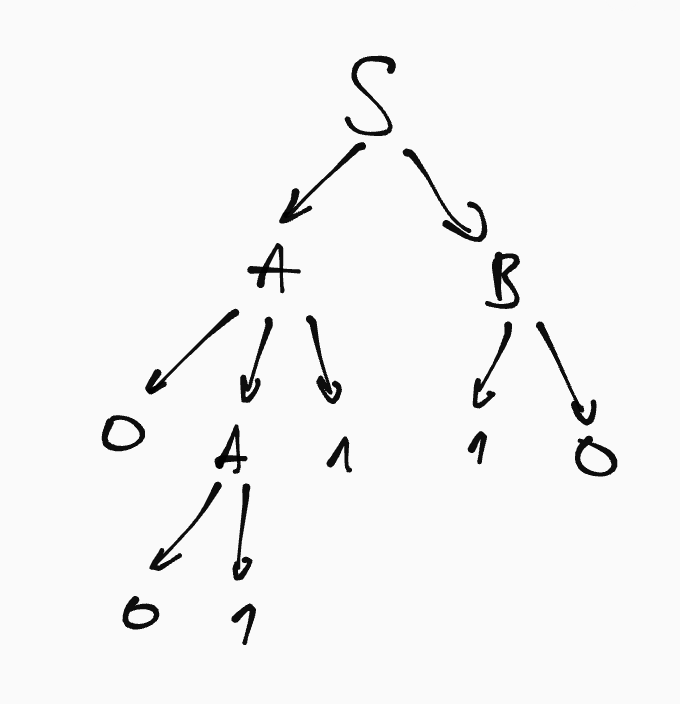
\includegraphics[width=0.5\linewidth]{04/4_1_a.png}


b)

$A$ generates $L_A = \{0^k1^k | k \geq{} 1\}$, $B$ generates $L_B = \{1^j0^j | j \geq{} 1\}$, and $S$ concatenates the two, so $L_S = \{0^k1^{k+j}0^j | j,k \geq{} 1\}$.\pagebreak
\subsection{Session 4, Exercise 2}

\lineparagraph{Exercise}

Consider

\begin{align*}
S \rightarrow& AS|A\\
A \rightarrow& 0A1|01
\end{align*}

\begin{enumerate}[(a)]
\item Give a parse tree and a leftmost derivation for word 01010011.
\item Determine the language generated by this grammar.
\end{enumerate}

\lineparagraph{Solution}\pagebreak
\subsection{Sessions 4 and 5, Exercise 3}

\lineparagraph{Exercise}

Give CF-grammars for the following languages. Are these unambiguous?

\begin{enumerate}[(a)]
\item $L = \{a^nb^{n+1}| n\geq{}0\}$
\item $L = \{a^nb^{2n} | n\geq{}0\}$
\item Palindromes over $\{a,b\}$
\item $L = \{a^ib^jc^k | (i = j \text{ or } i = k) \text{ and } i,j,k \geq{} 0\}$
\end{enumerate}

\lineparagraph{Solution}

(Multiple solutions can be correct here, we give one example for each.)

a)

\begin{align*}
    S \rightarrow& Tb\\
    T \rightarrow& aTb|\varepsilon
\end{align*}

$L_T = \{a^nb^n | n\geq{}1\}$, and $S$ just adds one more $b$ at the end. This language is unambiguous, since for \textbf{any} word in the grammar there is only a single possible (leftmost) derivation: we must always first use the $S \rightarrow Tb$ production rule, then the number of $a$'s and $b$'s determines the number of times the  $T \rightarrow aTb$ production rule is used, finally the $T \rightarrow \varepsilon$ must end the derivation.

Another good solution is $S \rightarrow aSb | b$, which does exactly the same thing with less rules.

b)

\begin{align*}
    S \rightarrow& aSbb|\varepsilon
\end{align*}

Since we now need twice as many $b$'s as $a$'s. This grammar is also unambiguous, since there is only one possible (leftmost) derivation for any word in the language: we use the $S \rightarrow aSbb$ as many times as there are $a$'s in the word, and then finally use $S \rightarrow \varepsilon$.

c)

\begin{align*}
    S \rightarrow& aSa | bSb | a | b |\varepsilon
\end{align*}

The matching characters in the palindromes are generated with rules $S \rightarrow aSa$ and $S \rightarrow bSb$, then if the palindrome is of odd length, the middle character is generated with rules $S \rightarrow a$ and $S \rightarrow b$, while if the palindrome is of even length, then no middle character is needed, so $S \rightarrow \varepsilon$ is used.

This grammar is unambiguous, since for any given palindrome, there is only one possible leftmost derivation for it: we read the input word from left-to-middle and when we see a character $a$ we must use production rule $S \rightarrow aSa$, when we see a $b$ we must use $S \rightarrow bSb$, then we take care of the middle character as we said before.

d)

\label{4f3d}

$L$ is the union of $L_1 = \{a^ib^ic^k | i,k \geq{} 0\}$ and $L_2 = \{a^ib^jc^i | i,j \geq{} 0\}$. So we can create a grammar by creating two independent grammars for $L_1$ and $L_2$ and combining them:

For $L_1$:
\begin{align*}
    X \rightarrow& TC\\
    T \rightarrow& aTb|\varepsilon\\
    C \rightarrow& cC|\varepsilon
\end{align*}

For $L_2$:
\begin{align*}
    Y \rightarrow& aYc|B\\
    B \rightarrow& bB|\varepsilon
\end{align*}

For $L=L_1\cup{}L_2$:

For $L_1$:
\begin{align*}
    S \rightarrow& X|Y\\
    X \rightarrow& TC\\
    T \rightarrow& aTb|\varepsilon\\
    C \rightarrow& cC|\varepsilon\\
    Y \rightarrow& aYc|B\\
    B \rightarrow& bB|\varepsilon
\end{align*}

This grammar is ambiguous, since the words of $a^ib^ic^i$ can be derived from both variable $X$ and variable $Y$ as well, so they have at least two leftmost derivations or parse trees.\pagebreak
\subsection{Session 4, Exercise 4}

\lineparagraph{Exercise}

Are the following grammars unambiguous? Are the languages generated by them unambiguous?

a)

\begin{align*}
S \rightarrow& aSa|bSb|aa|bb|a|b
\end{align*}

b)

\begin{align*}
S \rightarrow& TT|U \\
T \rightarrow& 0T|T0|\# \\
U \rightarrow& 0U00|\#
\end{align*}

\lineparagraph{Solution}\pagebreak
\subsection{Session 4, Exercise 5}

\lineparagraph{Exercise}

Let the alphabet be $\Sigma=\{0,1\}$, states of the pushdown automaton be $Q=\{A,B,C\}$, where $A$ is the start state, $C$ is the only accept state, let $Z$ be the start symbol of the stack. The transition function is the following:

\begin{align*}
    1.\text{ }\delta(A,0,\varepsilon) = \{(A,a)\}\\
    2.\text{ }\delta(A,1,\varepsilon) = \{(A, b)\}\\
    3.\text{ }\delta(A,\varepsilon,\varepsilon) = \{(B,\varepsilon)\}\\
    4.\text{ }\delta(B,0,a) = \{(B,\varepsilon)\}\\
    5.\text{ }\delta(B,1,b) = \{(B,\varepsilon)\}\\
    6.\text{ }\delta(B,\varepsilon, Z) = \{(C,\varepsilon)\}
\end{align*}

\begin{enumerate}[a)]
    \item Give the possible computations of the automaton on word 010.
    \item Does it accept word 0110?
    \item What is the language recognized by the automaton?
    \item Give a CF-grammar for this language.
\end{enumerate}

\lineparagraph{Solution}

a)

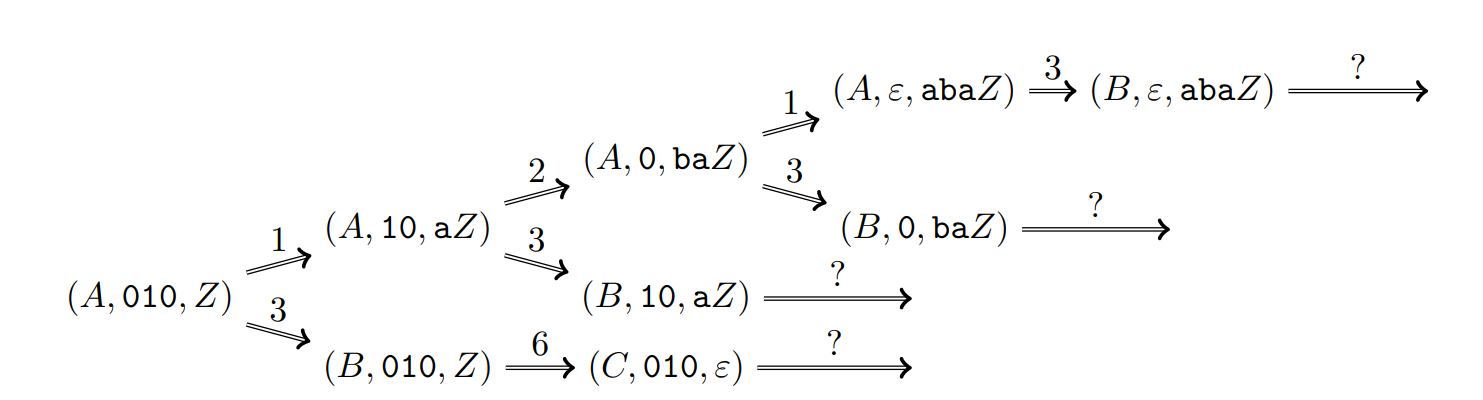
\includegraphics[width=\linewidth]{04/4_5_a.png}

b)

Yes, for example an accepting comutation (branch) is the following:


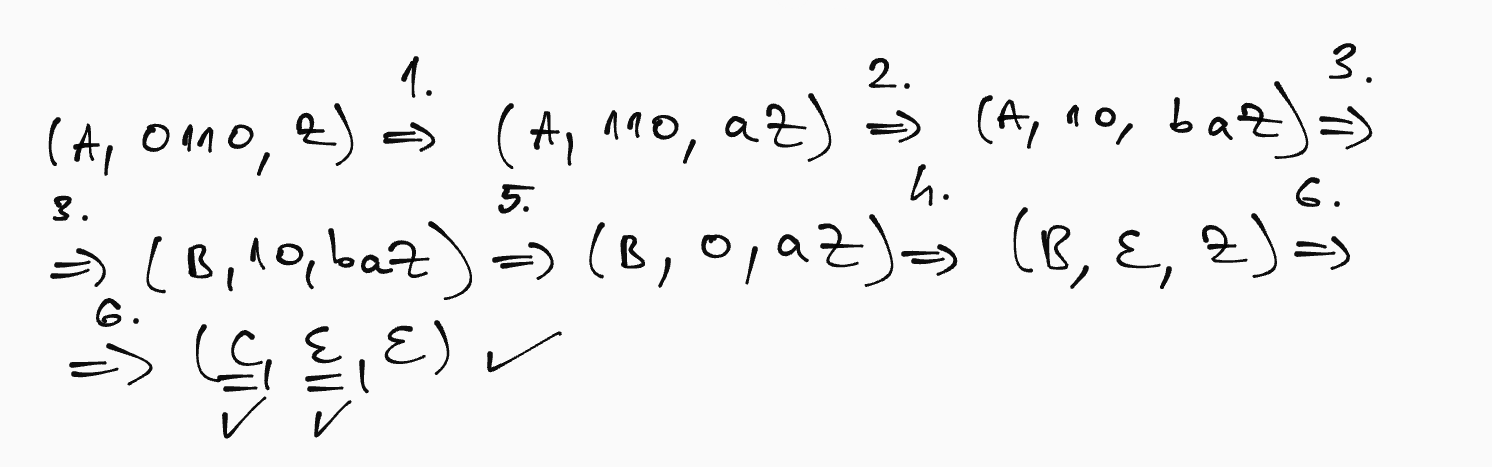
\includegraphics[width=\linewidth]{04/4_5_b.png}

c)

The language recognized is palindromes of odd length. These are accepted, since an accepting computation for these types of words will be: for the first half of the word transitions $1.$ and $2.$ will push the word ($0=a$, $1=b$) into the stack, then transition $3.$ will move to variable $B$, where the second (mirrored) half of the word will be compared to the first half on the stack using transitions $4.$ and $5.$. Since a stack is last-in-first-out, the comparisons will happen in the correct order. The stack can be emptied out this way and that allows for transition $6.$ to occur on the stack bottom symbol and move to the acceting $C$ state.

Words not in this language are rejected, since:
\begin{itemize}
    \item Only words of even length have a chance to be accepted, since the stack must be emptied out to move to the only accepting state and each character we put on the stack must have a pair that we use to remove it from the stack.
    \item Transition $3.$ must occur exactly at the middle of the word, for the same reason as stated above: if the word's length is $2n$, $n$ characters must be put on the stack, then move to state $B$, where $n$ characters must be removed from the stack. If the transition occurs too late, there will be remaining characters on the stack and we won't be able to move to state $C$, while if the transition occurs too early, the stack might be emptied out, however there will be remaining characters on he input so we could move to state $C$, however we won't accept since there are remaining characters on the input.
    \item If the word is not a palindrome, there must be at least one position where the character on it's mirrored position is wrong, either $a$ paired with a $b$ or $b$ paired with an $a$. This means, that when reading the stack back in state $B$, when we reach this position, we will have a wrong pairing: $0$ on the input with a character $b$ on the stack, or $1$ on the input with a character $a$ on the stack, for which no transition is defined from $B$, thus the machine will stop and the stack will not be empty, so we cannot move to state $C$ and $B$ is a rejecting state (plus, there will also be remaining input as well).
\end{itemize}

d)

\begin{align*}
    S \rightarrow& aSa | bSb | \varepsilon
\end{align*}

We have shown in previous exercises that this is indeed the grammar for palindromes of even length.\pagebreak
\subsection{Session 4, Exercise 6}

\lineparagraph{Exercise}

Construct a pushdown automaton for the language of palindromes.

\lineparagraph{Solution}

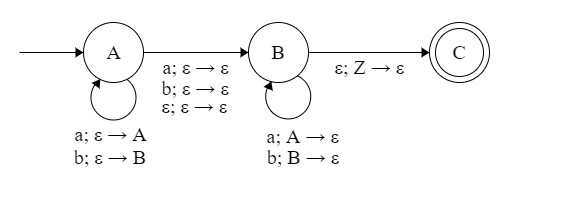
\includegraphics[width=0.5\linewidth]{04/4_6.png}

Proof:

States meaning:
\begin{itemize}
    \item State $A$ is used to read the first half of the word, and store it on the stack.
    \item State $B$ is used to read the second half of the word and compae it to the first half of the word on the stack.
    \item State $C$ can only be reached by emptying the stack out, so only palindromes can reach it.
\end{itemize}

Transitions:

\begin{itemize}
    \item State $A$'s loop transitions will store the corresponding characters on the stack.
    \item Transition from $A$ to $B$ takes care of the middle character, in case of an odd length palindrome, or is an epsilon transition in case of an even length palindrome.
    \item State $B$'s loop transitions will compare the second half of the word with the first half (mirrored, since a stack is a LIFO), and will only remove characters from the input and the stack if they match. If there is a character on the stack that doesn't match the PDA will halt in state $B$, which will reject.
    \item If the stack is emptied out we move to state $C$. In this case, if we read the entire input we can be sure that the word's first half matches the second half, and we will accept. If there are charaters remaining on the input, it means that not the entire word, only the prefix of the word was a palindrome, in which case the PDA correctly rejects, since there is still input remaining.
\end{itemize}

Accept / reject states:

The only accept state is state $C$ which can only be reached with no input remaining if the first half of the input is the mirror of the second half of the input. If a word is not a palindrome there won't be any accepting branch in the computation, all branches will end up in either $A$ (store the entire word), or $B$: start comparing too late, stack is not empty to move to $C$, or $C$ but with input remaining, since we started comparing too early.\pagebreak
\subsection{Session 4, Exercise 7}

\label{4_7}

\lineparagraph{Exercise}

Create pushdown automata for the following languages.
\begin{enumerate}[a)]
    \item $L_a = \{a^ib^jc^k | i,j,k \geq{} 0\text{ and }i+j = k\}$
    \item $L_a = \{a^ib^jc^k | i,j,k \geq{} 0\text{ and }j+k = i\}$
    \item $L_a = \{a^ib^jc^k | i,j,k \geq{} 0\text{ and }i+k = j\}$
\end{enumerate}


\lineparagraph{Solution}

a)

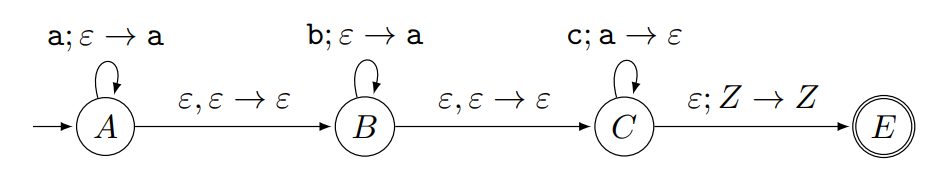
\includegraphics[width=\linewidth]{04/4_7_a.png}

TODO Proof

b)

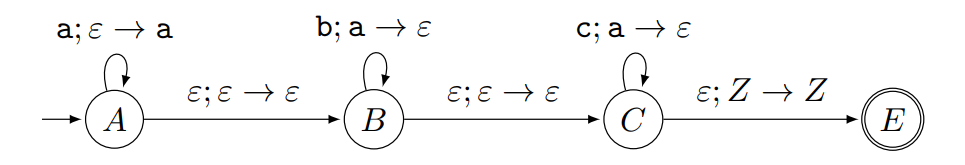
\includegraphics[width=\linewidth]{04/4_7_b.png}

TODO Proof

c)

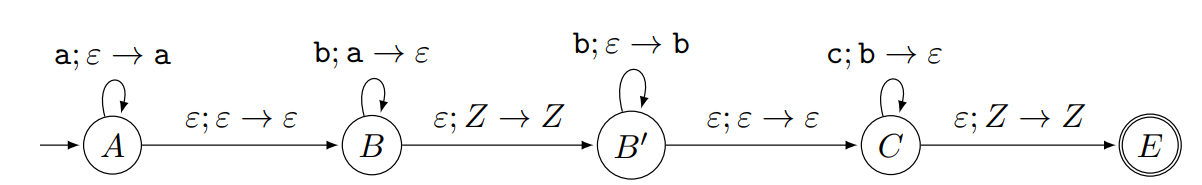
\includegraphics[width=\linewidth]{04/4_7_c.png}

TODO Proof

Note: c) is the tricky one, since we need the number of $a$'s plus the number of $c$'s to be equal to the number of $b$'s, but the $b$'s come in-between the $a$'s and the $c$'s. In this case we split the processing of $B$'s into two parts: in the first part we compare the number of $b$'s to the $a$'s that came before, while in the second part we store the number of $b$'s to be compared with the number of the upcoming $c$'s.

In this case we used non-determinism heavily, since the transition between $B$ and $B'$ must happen at the correct time for the calculation to work: one computational branch will time it correctly and that one can become an accepting branch (if everything else is correct with the word).\pagebreak
\subsection{Sessions 4 and 5, Exercise 8}

\lineparagraph{Exercise}

Create a pushdown automaton for the language of proper parenthesisations.

\lineparagraph{Solution}

Idea: correct parenthesisation can be checked by counting from left to right: start with $0$ and add $+1$ for every $($ encountered and $-1$ for every $)$ encountered. The parenthesisation is correct if the sum never drops below $0$ during the calculation (too many $)$ in that case at that point) and at the end it equals to $0$. A simple PDA can be constructed to do exactly this calculation.


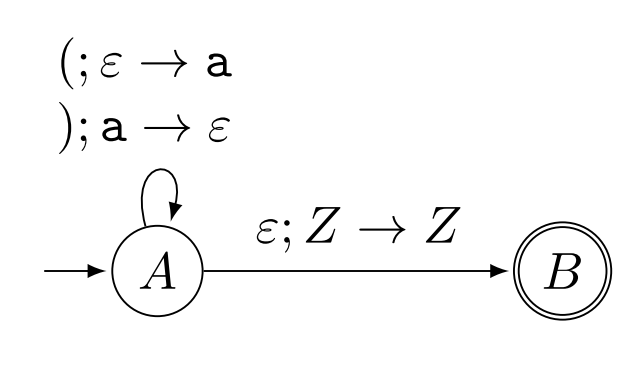
\includegraphics[width=0.4\linewidth]{04/4_8.png}

TODO Proof\pagebreak
\subsection{Sessions 4 and 5, Exercise 9}

\label{4_9}

\lineparagraph{Exercise}

Construct pushdown automata for the following languages.

\begin{enumerate}[a)]
\item $L_a = \{a^nb^m | 2n = m \geq{} 1\}$
\item $L_b = \{a^nb^m | 2n \geq{} m \geq{} n \geq{} 1\}$
\end{enumerate}

\lineparagraph{Solution}

a)

The first one is simpler, since we need to check for twice as many $b$'s as $a$'s. We can count the number of $a$'s in the stack with TWO tokens instead of one, so then the number of tokens in the stack must be equal to the number of $b$'s.

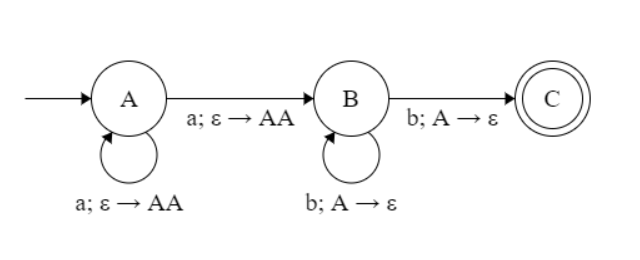
\includegraphics[width=0.5\linewidth]{04/4_9_a.png}

To enforce that the loops run at least once, due to the requirement that $n,m\geq{}1$ ($n\geq{}0.5$ is the same as $n\geq{}1$, since $n$ is an integer), we used non-epsilone transitions between the states, and copied the loop's transition to the existing transitions from the states as well.

TODO Proof

b)

The second one is more complex, since the number of $b$'s is now anywhere between $2n$ and $n$! How do we enforce $2n \geq{} m \geq{} n$? We just did it with $2n = m$, also if it were only $n = m$, we could replace the $a; \varepsilon \rightarrow AA$ transitions with  $a; \varepsilon \rightarrow A$ transitions. But how do we check for in-between these two numbers?

We will rely on non-determinism again:

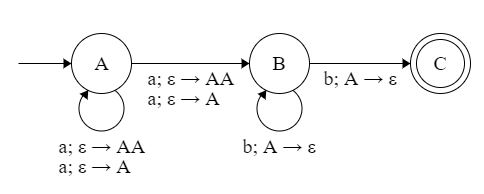
\includegraphics[width=0.5\linewidth]{04/4_9_b.png}

We use both $a; \varepsilon \rightarrow A$ and $a; \varepsilon \rightarrow AA$. The PDA will nondeterministically use either the first or the second transition and push either 1 or 2 $A$'s on the stack. So the number of $A$'s on the stack will be anywhere between $2n$ and $n$, and there will exist a computational branch (if the word is in the language) where their number will be equal to $m$ and the word will be accepted.\pagebreak
\subsection{Sessions 4 and 5, Exercise 10}

\lineparagraph{Exercise}

TODO

\lineparagraph{Solution}

TODO\pagebreak
\subsection{Sessions 4 and 5, Exercise 11}

\lineparagraph{Exercise}

TODO

\lineparagraph{Solution}

TODO\pagebreak
\subsection{Session 4, Exercise 12}

\lineparagraph{Exercise}

TODO

\lineparagraph{Solution}

TODO\pagebreak

\section{March 23th (Session 5): Turing-machines}
\subsection {Session 5, Exercise 1}

\lineparagraph {Exercise}

Create a PDA from the grammar $S \rightarrow aSa|bSb|aa|bb|a|b$ and give an accepting computation for the word $ababa$ (if such one exists).

\lineparagraph {Solution}

a)

Using the schema for turning a CF-grammar into a PDA:

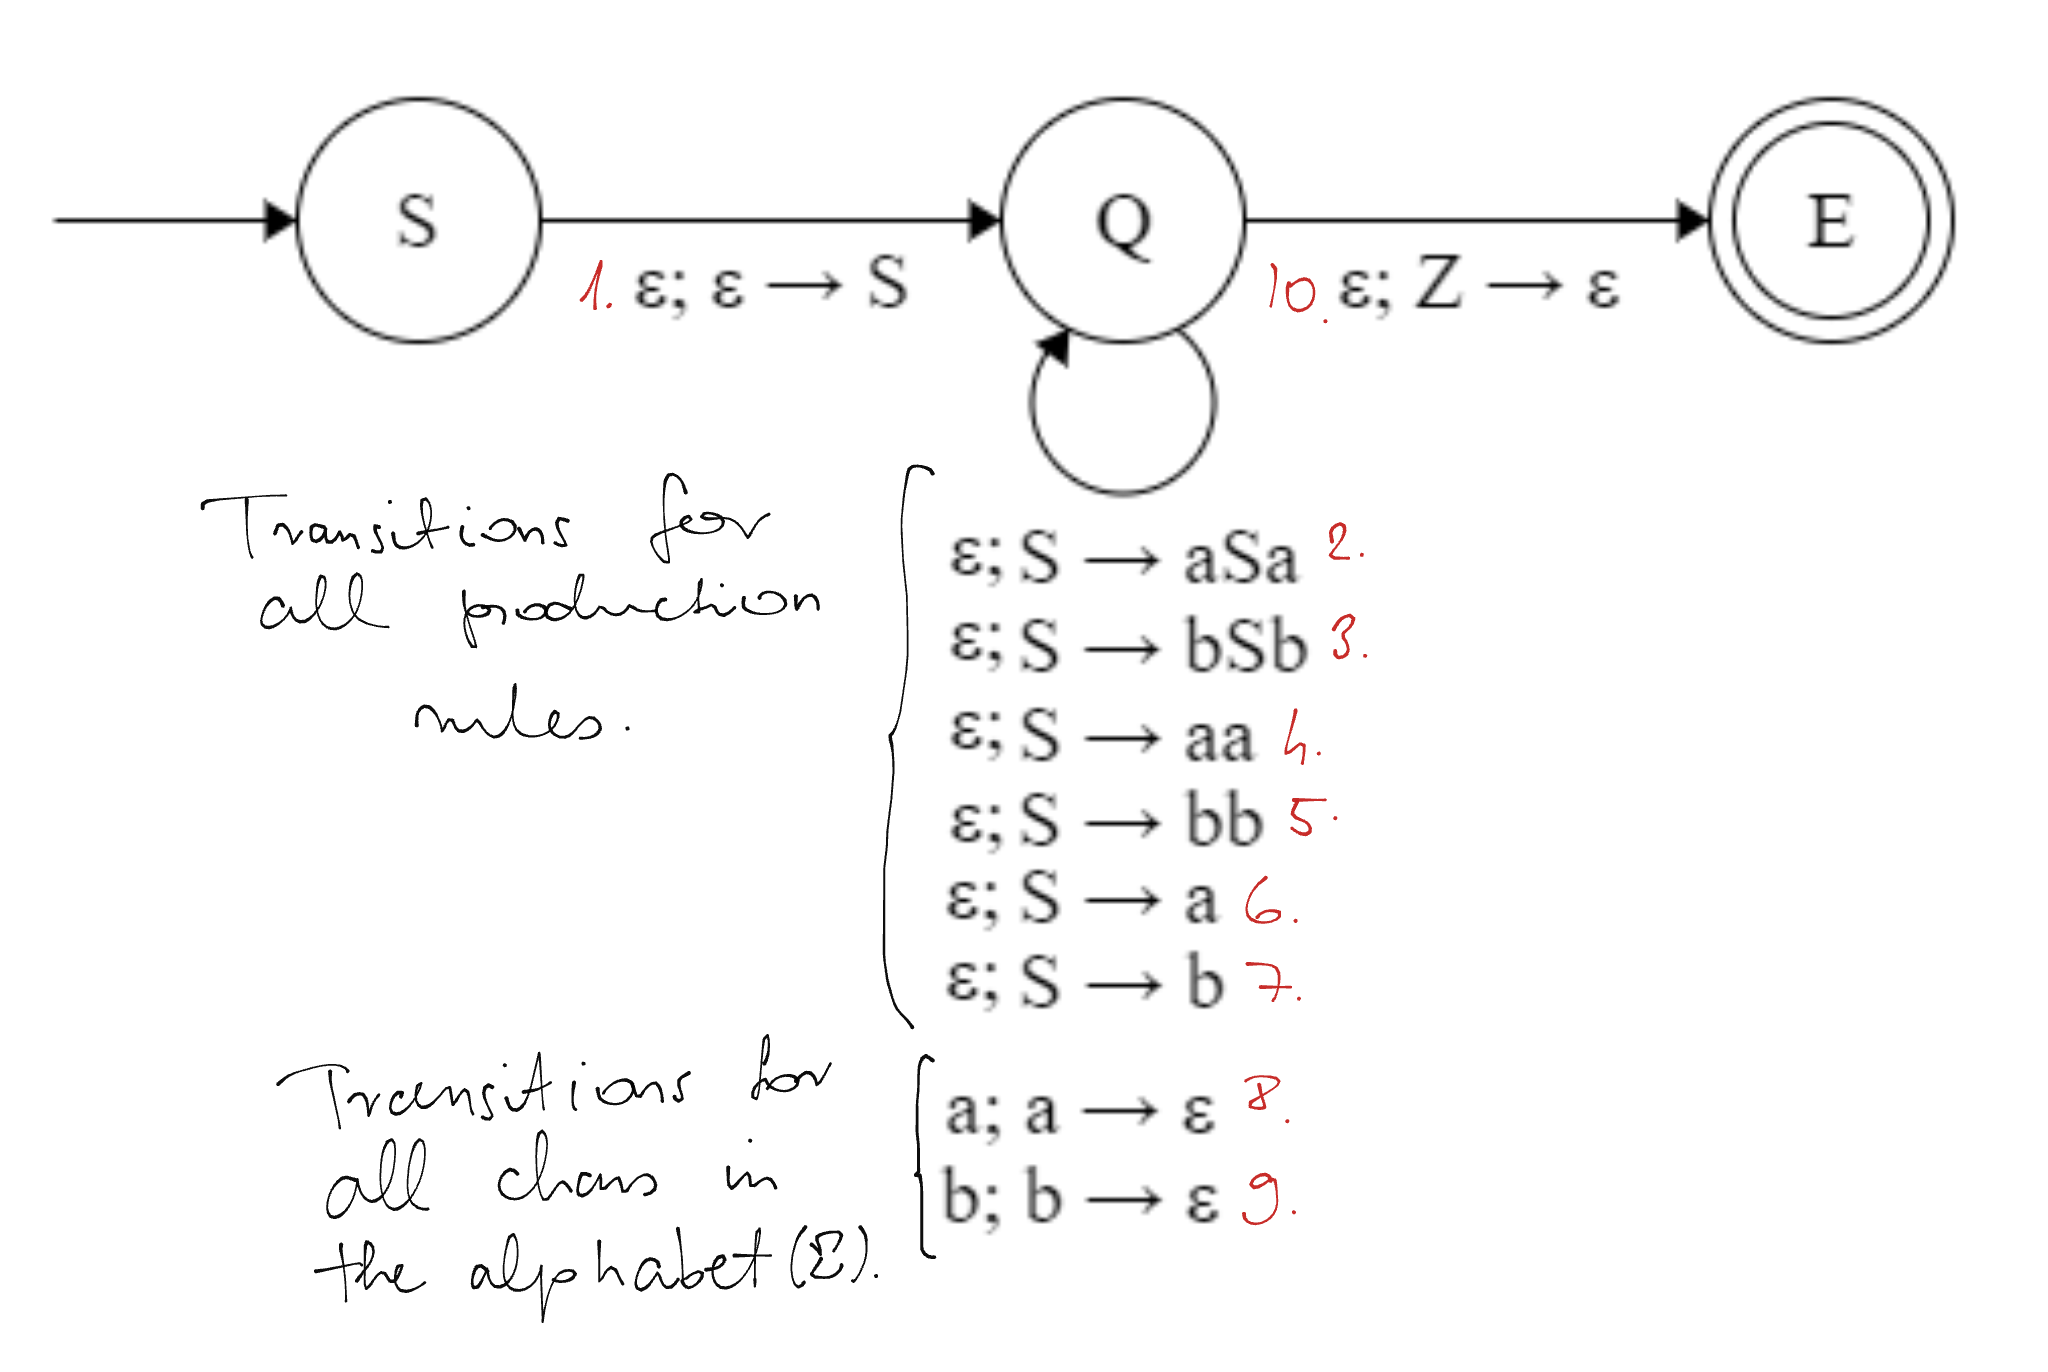
\includegraphics[width=\linewidth]{05/6_1.png}

\begin{itemize}
    \item Transition 1: First, we put the starting variable $S$ on top of the stack.
    \item Transitions 2-7: For all production rules in the grammar we add transitions, which will take care of doing the (leftmost) derivation inside the stack, while not reading from the input.
    \item Transitions 8-9: For all letters in the alphabet we add production rules, which will take care of comparing the input with the derived word in the stack.
    \item Transition 10: Finally we check if the stack is empty and only move to the accept state $E$ if it is.
\end{itemize}

b)

Accepting computation for $ababa$:

$(S, ababa, Z)
\xrightarrow{1.} (Q, ababa, SZ)
\xrightarrow{2.} (Q, ababa, aSaZ)
\xrightarrow{8.} (Q, baba, SaZ)
\xrightarrow{3.} (Q, baba, bSbaZ)
\xrightarrow{9.} (Q, aba, SbaZ)
\xrightarrow{6.} (Q, aba, abaZ)
\xrightarrow{8.} (Q, ba, baZ)
\xrightarrow{9.} (Q, a, aZ)
\xrightarrow{8.} (Q, \varepsilon, Z)
\xrightarrow{10.} (E, \varepsilon, \varepsilon)$
\pagebreak
\subsection {Session 5, Exercise 2}

\lineparagraph {Exercise}

Let the transition function of the 1-tape Turing-machine be

\begin{align*}
    \delta(q_0,1) = (q_1,1,R)\\
    \delta(q_0,*) = (q_2,*,R)\\
    \delta(q_1,1) = (q_3,1,R)\\
    \delta(q_3,1) = (q_0,1,R)
\end{align*}


start state is $q_0$, accept state is $q_3$. What is the language recognized by this machine?

\lineparagraph {Solution}

It's easier to see what's happening if we draw the machine:

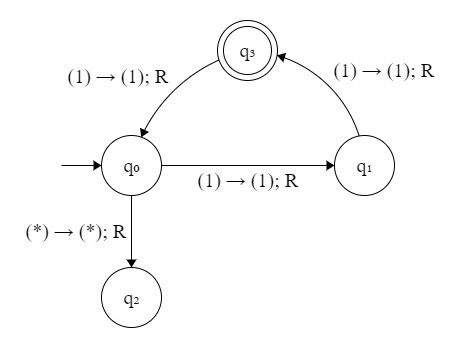
\includegraphics[width=0.5\linewidth]{05/6_2.png}

It the $q_0, q_1, q_3$ cycle reads the input word on the tape from left to right and counts the number of $1$'s modulo $3$. In $q_0$ the remainder is $0$, in $q_1$ the remainder is $1$ and in $q_3$ the remainder is $2$.

When the input is $\varepsilon$ (the empty string) the $q_0 \xrightarrow{(*) \rightarrow (*);\text{ }R} q_2$ transition will move the machine to $q_2$ and it will halt there, since there is no transitions defined, thus reject the empty string input. (This transition could have been left out, since then the machine would remain in $q_0$ and reject the empty string input similarly.)

Since the accept state is $q_3$, words containing $3k+2$ number of $1$'s will be accepted, where $k\geq{}0$.

Notice how the above Turing-machine does exactly the same thing as this Finite Automaton:

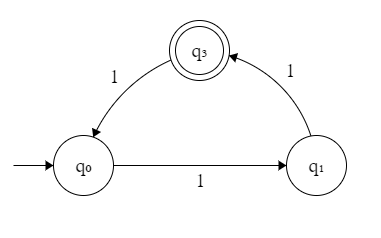
\includegraphics[width=0.6\linewidth]{05/6_2_b.png}

We have seen similar modulo counter automatons on the first practice session.\pagebreak
\subsection {Session 5, Exercise 3}

\label{6f3}

\lineparagraph {Exercise}

The following table contains the transition function of a 2-tape Turing machine, where $*$ is the blank symbol on the tapes, and $q_0$ is the start state.

\begin{center}
\includegraphics[width=0.7\linewidth]{05/6_3_task.png}
\end{center}

\begin{enumerate}[a)]
    \item What is the content of tape 2 when the machine moves to state $q_2$?
    \item What is the language $L(M)$ if the only accept state is $q_5$?
    \item At most how many steps are done by the machine on an input of length $n$ before it stops?
\end{enumerate}

\lineparagraph {Solution}

To see a little bit easier what this TM does, I converted it line-by-line to the below form:

\includegraphics[width=\linewidth]{05/6_3_canvas.png}

What this does:
\begin{itemize}
    \item Transition 3: This one handles the empty string input and immediately moves to the accept state $q_5$. So the empty string is accepted. So the empty string is accepted in $1$ step. For any other input, the following happens:
    \item Transitions 1-2: They put down an $X$ character at the beginning of the second tape. This $X$ will be used later to make sure that the head does not fall of the tape (moving from the first position to the left would cause the head to fall off, this $X$ is there so we can detect it and make sure no transition is defined that moves the 2nd head to the left when it reads an $X$). This is $1$ step.
    \item Transitions 4-5: They copy the first tape's contents to the second tape. This is $n$ steps if the input is of length $n$.
    \item Transition 6: When the on the first tape the head is at the end of the input word (sees the $* =$ empty cell character we move to state $q_2$ and we position the second head on the last character of the copied input. (While the first head remains on the $* =$ empty cell after the input.) This is $1$ step.
\end{itemize}

a) When we move to state $q_2$ the contents of tape $2$ will be the character $X$ at the beginning, then the input word copied afterwards.

\begin{itemize}
    \item Transitions 7-8: The first head stays on the same $*$ cell, while the second had moves to the left until it finds the character $X$ (beginning of the second tape). This is $n$ steps if the input is of length $n$.
    \item Transition 9: The first head is positioned at the end of the input word, while the second head is positioned at the beginning of the (copied) input word. This is $1$ step.
    \item Transitions 10-15: Together these make $2n$ steps for an input word of length $n$, see explanation below:
    \begin{itemize}
        \item Transitions 10-11: These compare the two strings (the input word twice, on the first tape from right to left and on the second tape from left to right). However, the first head is not moved immediately to the left. This is because the first head could fall off the first tape, since there is no protective $X$ there. We cannot recklessly move to the left.
        \item Transitions 12-15: Instead we lag behind the second head and make sure that the second head reads either a $0$ or a $1$ (and the first head can read $0$ or $1$ as well), which means that the word has not yet ended! (The second head would read $*$ here when the word ends.) This means that it is \textbf{safe} to move the first head to the left, since it is not yet at the beginning of the tape, so we move.
    \end{itemize}
    \item Transitions 16-17: Finally, when the second head reads the empty cell, it means that the word has ended (and has been successfully compared), so we can move to $q_5$. We make sure that we \textbf{DO NOT} move the first head to the left in this step, since it would fall off. Since the first head could be on a character $0$ or a $1$ we need to define 2 transitions to cover all possibilities. We move to $q_5$ here. This is $1$ step.
\end{itemize}

Together the number of steps for a successfull computation has been (for a non-empty input):

\begin{itemize}
    \item Transitions 1-2: $1$ step.
    \item Transitions 4-5: $n$ steps.
    \item Transition 6: $1$ step.
    \item Transitions 7-8: $n$ steps.
    \item Transition 9: $1$ step.
    \item Transitions 10-15: $2n$ steps.
    \item Transitions 16-17: $1$ step.
\end{itemize}

At most $4n+4$, but keep in mind that for a rejecting computation the number of steps is smaller, depending on where it halts in transitions 10-15. (At least $2n+3$ steps, since copying and moving the second head back to the first position will be done regardless of rejecting / accepting.)\pagebreak
\subsection {Session 5, Exercise 4}

\lineparagraph {Exercise}

Let language L consist of words over $\{0,1\}$ whose middle character is $0$. Prove that L is CF.

\lineparagraph {Solution}

We prove that $L$ is CF by giving a CF-grammar. (We could also give a PDA.)

\begin{align*}
    S \rightarrow& 0S0 | 0S1 | 1S0 | 1S1 | 0
\end{align*}

This grammar is similar to the odd-palindrome one, however we allow all possible combinations of letters. But the middle one must be a $0$.

Proof: this CF-grammar generates $L$.

Any word in the language has to be of odd length. We look at the first and last characters and use one of the four transitions from $S \rightarrow 0S0 | 0S1 | 1S0 | 1S1$ to generate them, then we remove those from the word and keep repeating until $1$ character is left. This character is the middle one, since we removed an equal number of characters before and after it ($1$-$1$ in each step), so it has to be a $0$, which can be generated using production rule $S \rightarrow 0$.

Any word outside of this language is either:
\begin{itemize}
    \item of even length, in which case there is no possilbe way for this grammar to generate it, since rules  $S \rightarrow 0S0 | 0S1 | 1S0 | 1S1$ generate an even number of characters, while the  $S \rightarrow 0$ rule ends the derivation and can be used only once, which results in an odd lenght word. This includes the $\varepsilon$ (empty string), which cannot be generated, since there is no $S \rightarrow \varepsilon$ rule.
    \item of odd length, but with the $1$ middle character. Using the previous explanation, since there is no  $S \rightarrow 1$ rule, there is no way to put a $1$ in the middle, so these words can't be generated either.
\end{itemize}

We have shown that this grammar generates \textbf{the correct words} and \textbf{only the correct words = does not generate words outside of the language}.\pagebreak
\subsection {Session 5, Exercise 5}

\label{6f5}

\lineparagraph {Exercise}

Give a Turing-machine for the language

\begin{align*}
 L = \{w\#w | w \in{} \{0,1\}^*\}.
\end{align*}

Give an upper bound for the running time.

\lineparagraph {Solution}

This is the Turing-machine:

\includegraphics[width=\linewidth]{05/6_5.png}

Proof: This machine's language is $L$.

States and transitions:
\begin{itemize}
    \item State $s$: The starting state, the empty string will remain here.
    \item Transitions $1$ and $2$: will put an $X$ at the beginning of the second tape, for protection against failling off.
    \item State $m$: Used for copying the input word up until the first $\#$ to the second tape.
    \item Transitions 3-4: Copy a $0$ or a $1$ to the second tape, move both heads to the next position.
    \item Transition 5: When we encounter the first $\#$ we stop copying and move to state $v$, while positioning the second head back to the last copied character. If there is no $\#$ in the word the computation halts in state $m$ and rejects the input correctly.
    \item State $v$: Used for moving the second head back to the beginning of the second tape.
    \item Transitions 6-7: The first head will stay on the character $\#$, while the second head moves to the left while it sees a $0$ or a $1$.
    \item Transition 8: When the second head sees the $X$ at the beginning of the second tape it reached the beginning of the tape. The heads are positioned, so the first head is at the beginning of the (copied) input, while the second head is at the first character after the $\#$ in the input.
    \item State $h$: Used to compare the first part of the input (before the $\#$) to the second part of the input (after the $\#$).
    \item Transitions 9-10: We make sure that all characters match in the fist and the second part of the inputa word, so that it is in $w\#w$ form.
    \item Transition 11: Only allows moving to the accepting $e$ state if the the two heads reach the empty cells at the same time = if the two parts of the input word match. If the word contains another $\#$, or if the two parts don't match, then this transition won't be able to fire and we won't be able to move to state $e$.
    \item State $e$: Only words in the language can reach this state to accept. No further computation needed.
    \item Transition 12: There is a special word, $\#$, which the generic computation above cannot handle, since it has no $0$ or $1$ characters, however it should be accepted, since $w$ is allowed to be the empty string. We handle this case specially, we detect that on the input we see the $\#$ character, and
    \item Transition 13: Detects that there is no further characters in the input, so the input word is $\#$ exactly.
    \item States $u1$ and $u2$: Used for handling this special case, $u2$ will accept the $\#$ only.
\end{itemize}

Accepting / rejecting states, accepted / rejected words:

\begin{itemize}
    \item If the word starts with $\#$ character it is moved to $u1$. It can only be accepted if the word is $\#$ exactly, no further characters can come. $\#$ is moved to $u2$ and accepted, while the others remain in $u1$ and get rejected there.
    \item If the word starts with some $0$ or $1$ characters, those get copied to the second tape.
    \item If the word contains no $\#$ character then it stops in state $m$ and gets rejected.
    \item If the word contains a $\#$ character, the characters coming after should match what characters were before. So any word in the form $w\#w$ is accepted, however any $w\#h$, where $w\neq{}h$ will stop in state $h$ and will be rejected. This includes the words that contain more $\#$'s (in $h$) and words that contain only $0$'s and $1$'s in $h$, but not match $w$, since the only possible way to activate transition 11 is to have matching characters before the $\#$ and after it. State $e$ accepts these words.
\end{itemize}

Upper bound for the running time: the longest running time will be an accepted word that reachers state $e$. If the word is $w\#w$, of lenght $n=2k+1$, so that $w$ is of length $k$, then:

\begin{itemize}
    \item Transitions 1-2: $1$ step, to put down an $X$.
    \item Transitions 3-4: $k$ steps, to copy $w$ to the second tape.
    \item Transition 5: $1$ step to detect the $\#$ and position.
    \item Transitions 6-7: $k$ steps to move the second head to the first position on the second tape.
    \item Transition 8: $1$ step to detect the beginning of the second tape and position the heads.
    \item Transitions 9-10: $k$ steps to compare the two parts.
    \item Transition 11: $1$ step to see that they end at the same time.
\end{itemize}

$1+k+1+k+1+k+1 = 3k+4$ steps, where $n=2k+1$, so $k=\frac{n}{2}-1$, so $3k+4 = 3(\frac{n}{2}-1)+4 = \frac{3n}{2}+1 \in{} O(n)$. For accepted words this is $\Theta(n)$, for rejected words not necessarily, for example the input word $\#0^k$, for any large $k$ will be rejected after $1$ step, in $u1$.\pagebreak
\subsection {Session 5, Exercise 6}

\lineparagraph {Exercise}

Let $L_r$ be an arbitrary regular language and let $L_c$ be an arbitrary CF language.
\begin{enumerate}
    \item Show an example when $L_r \cap L_c$ is not regular.
    \item Prove that $L_r \cap L_c$ is always context-free.
    \item Show an example when $L_1$ and $L_2$ are both context-free but $L_1 \cap L_2$ is not.
\end{enumerate}

\lineparagraph {Solution}

a)

For example if we take $L_r = \Sigma^*$, which is regular. Then, we take a known non-regular, but CF language, $L_c = \{a^nb^n | n \geq{} 0\}$. Ther instersection is $L_c$ itself, which is not regular, but CF.

b) If $L_r$ is regular, there exists a DFA that accepts it, let's call this $M_r$. Then, since $L_c$ is CF, there exists a PDA that accepts it, let's call this $M_c$. To show that $L_r \cap L_c$ is CF we construct a PDA from $M_r$ and $M_c$ that accepts it.

The main idea is to take all the possible pairs of states, where one state comes from $M_r$ and the other from $M_c$. For a given input character, we define the transition function, so that ''it keeps track of what's happening in both $M_r$ and $M_c$ at the same time'', for each statepair $(q_r, q_c)$, by checking what $M_r$ would do for the given input character in state $q_r$ and what would $q_c$ do, and moving to that statepair (or, since the PDA can have a set of possible states it moves into, the set of all statepairs).

We keep track of what's happening in $M_c$'s stack in the stack we have (this is why we cannot do this for two CF-languages, we would need to keep track of two stacks).

The starting statepair is going to be the statepair which contains the starting states from their respective machines.

The accepting statepairs will be the ones for which both states accept in their respective machines, since we need $L_r \cap L_c$.

The PDA constructed in this way will accept $L_r \cap L_c$, which means that the language is CF.

c)

These languages are both CF:

$L_1 = \{a^nb^nc^k | n,k \geq{} 0\}$ (Number of $a$'s and $b$'s is equal.)

$L_2 = \{a^ib^jc^j | i,j \geq{} 0\}$ (Number of $b$'s and $c$'s is equal.)

(See \ref{4f3d} for a CF-grammar for $L_1$, and based on that $L_2$ can be constructed in a similar manner.)

$L_1 \cap L_2 = \{a^nb^nc^n\}$  (Number of $a$'s and $b$'s and $c$'s is equal.)

Which is known to be non-CF. (The idea behind this is that we would need to use the stack to keep track of the number of $a$'s, but we would throw them out when comparing them with the number of $b$'s and there will be nothing left to compare to when the $c$'s come. The formal proof is more complicated and outside of the scope of this class.)\pagebreak
\subsection {Session 5, Exercise 7}

\lineparagraph {Exercise}

Sketch a Turing machine for the following languages. It is not neccessary to give the transition function precisely, it is enough to describe (in details) the idea of the working of the TM.

\begin{enumerate}[a)]
    \item $L_1 = \{a^nb^m | 2n = m \geq{} 1\}$
    \item $L_2 = \{a^ib^jc^k | i,j,k \geq{} 1, i+j = k\}$
    \item $L_3 = \{a^ib^jc^k | i,j,k \geq{} 1, i \cdot j = k\}$
\end{enumerate}

\lineparagraph {Solution}

I'm giving the TM's precisely, but you could just describe them. (Basically what the itemized list contains below, without referencing the specific index of the transitions.)

a) Similar to \ref{4f9} a), but now we need to give a TM, instead of a PDA:

\includegraphics[width=\linewidth]{05/6_7_canvas.png}

\begin{itemize}
    \item Transition 1: We mark the beginning of the second tape with an $X$, so we don't fall off later.
    \item Transitions 2-3: For every $a$ character on the first tape we copy it twice to the second tape. Pay attention: in transition 2 the first head doesn't move, but in transition 3 it does.
    \item Transition 4: When the $a$'s are done and the $b$'s are coming we position the second head to the end of the copied $a$'s.
    \item Transition 5: We compare the number of $a$'s and $b$'s on the second and first tape. They have to be equal, which means that the original input had to have half as many $a$'s as $b$'s.
    \item Transition 6: If the first head reaches the end of the input at the same time the second head reaches the beginning of the second tape (marked with the $X$), it means that the number of $a$'s and $b$'s is correct and the word can be accepted.
\end{itemize}

b) Same as \ref{4f7}, but now we need to give a TM, instead of a PDA:

\includegraphics[width=\linewidth]{05/6_7_b_canvas.png}

\begin{itemize}
    \item Transition 1: We mark the beginning of the second tape with an $X$, so we don't fall off later.
    \item Transition 2: Copy the $a$'s to the second tape.
    \item Transition 3: Detect that the $b$'s are coming.
    \item Transition 4: Copy the $b$'s to the second tape, copy them as $a$'s since we only care about their collective numbers and this spares us one extra transition (similar to transition 6, but for a $b$).
    \item Transition 5: Detect that the $c$'s are coming.
    \item Transition 6: Compare the number of $a$'s and $b$'s = the number of $a$'s on the second tape to the number of $c$'s.
    \item Transition 7: If we run out of $a$'s and $c$'s at the same time it means that there were an equal number of them, so we can accept the input.
\end{itemize}

Important: Transition 1,3 and 5 enforce that $i,j,k \geq{} 1$.

c) 

The idea is to: Use 3 tapes, mark the beginning of the second and third tape. Copy the $a$'s to the first tape. Then step on the first $a$ on the second tape and run through the first tape copying all of the $b$'s to the third tape. Now step to the left on the second tape, and do the same for the next $a$, and do it until there are $a$'s left. When you reach the $X$ mark on the second tape, the third tape will contain $i \cdot j$ $b$'s. Now compare the number of $b$'s on the third tape to the remaining $c$'s on the first tape.

It is important to keep in mind that for an odd number of $a$'s the head on the first tape will be at the last $b$ (next to the $c$), while for an even number of $a$'s the head on the first thape will be at the first $b$ (not next to the $c$). Handle the latter case by moving the first head to the right until it sees a $c$.\pagebreak
\subsection {Session 5, Exercise 8}

\lineparagraph {Exercise}

\lineparagraph {Solution}
\pagebreak
\subsection {Session 5, Exercise 9}

\lineparagraph {Exercise}

\lineparagraph {Solution}
\pagebreak

\section{March 30th (Session 6): Turing-machines 2}
\subsection {Session 6, Exercise 1}

Same as \ref{6f3}.\pagebreak
\subsection{Session 6, Exercise 2}

\lineparagraph{Exercise}

A 2-szalagos $M$ Turing-gép átmeneti függvényét a következő táblázat írja le, ahol * jelöli a szalagon az üres jelet és $q_{0}$ a kezdő állapotot:

\begin{tabular}{|c|c|c||cc|cc|c|}
\hline állapot & 1. szalag & 2. szalag & 1. szalag & 2. szalag & új állapot \\
\hline$q_{0}$ & 0 & $*$ & 0 & $\mathrm{H}$ & $\mathrm{X}$ & $\mathrm{J}$ & $q_{1}$ \\
& 1 & $*$ & 1 & $\mathrm{H}$ & $\mathrm{X}$ & $\mathrm{J}$ & $q_{1}$ \\
& $*$ & $*$ & $*$ & $\mathrm{H}$ & $*$ & $\mathrm{H}$ & $q_{5}$ \\
\hline$q_{1}$ & 0 & $*$ & 0 & $\mathrm{~J}$ & 0 & $\mathrm{~J}$ & $q_{1}$ \\
& 1 & $*$ & 1 & $\mathrm{~J}$ & 1 & $\mathrm{~J}$ & $q_{1}$ \\
& $*$ & $*$ & $*$ & $\mathrm{H}$ & $*$ & $\mathrm{~B}$ & $q_{2}$ \\
\hline$q_{2}$ & $*$ & 0 & $*$ & $\mathrm{H}$ & 0 & $\mathrm{~B}$ & $q_{2}$ \\
& $*$ & 1 & $*$ & $\mathrm{H}$ & 1 & $\mathrm{~B}$ & $q_{2}$ \\
& $*$ & $\mathrm{X}$ & $*$ & $\mathrm{~B}$ & $\mathrm{X}$ & $\mathrm{J}$ & $q_{3}$ \\
\hline$q_{3}$ & 0 & 0 & 0 & $\mathrm{H}$ & 0 & $\mathrm{~J}$ & $q_{4}$ \\
& 1 & 1 & 1 & $\mathrm{H}$ & 1 & $\mathrm{~J}$ & $q_{4}$ \\
\hline$q_{4}$ & 0 & 0 & 0 & $\mathrm{~B}$ & 0 & $\mathrm{H}$ & $q_{3}$ \\
& 0 & 1 & 0 & $\mathrm{~B}$ & 1 & $\mathrm{H}$ & $q_{3}$ \\
& 1 & 0 & 1 & $\mathrm{~B}$ & 0 & $\mathrm{H}$ & $q_{3}$ \\
& 1 & 1 & 1 & $\mathrm{~B}$ & 1 & $\mathrm{H}$ & $q_{3}$ \\
& 0 & $*$ & 0 & $\mathrm{H}$ & $*$ & $\mathrm{H}$ & $q_{5}$ \\
& 1 & $*$ & 1 & $\mathrm{H}$ & $*$ & $\mathrm{H}$ & $q_{5}$ \\
\hline
\end{tabular}

(a) Mi a 2. szalag tartalma, amikor a gép $q_{2}$ állapotba kerül?

(b) Mi az $L(M)$ nyelv, ha $q_{5}$ az egyetlen elfogadó állapot?

(c) Legfeljebb hány lépést tehet a gép egy $n$ hosszú bemeneten, mielőtt megáll?

\lineparagraph{Solution}

Nézzük, mi történik:

$q_{0}:$ Ha nem üres a bemenet, akkor egy $X$ kerül a 2. szalagra (ez jelzi majd a szalag elejét).

$q_{1}$ : Lemásolja az 1. szalagon talált karaktert a 2. szalagra. Akkor lép csak ki innen, ha a bemenet végére ért (ekkor, ha az elsö szalagon a $w$ szó van, akkor a 2. szalagon $X w$ ). Ilyenkor következik a $q_{2}$ állapot, ahova úgy lépünk át, hogy az 1. szalagon maradunk az első üres mezón, a 2. szalagon visszalépünk az utolsónak írt karakterre.

$q_{2}:$ Az első szalagon nem mozdulunk, mialatt visszamegyünk a 2 . szalag elejére. Végül úgy lépünk át $q_{3}$-ba, hogy az 1. szalagon egyet visszalépünk (az utolsó nem üres mezóre), a 2. szalagon egyet elóre lépünk (az elsö nem $X$ karakterre). $q_{3}$ : Ha ugyanazt látjuk mindkét szalagon, akkor az elsőn nem mozdulunk, a másodikon egyet előre lépünk és átkerülünk $q_{4}$-be. (Elsớ alkalommal tehát az 1. szalag utolsó és a 2. szalag $X$ utáni elsö karakterét, azaz a $w$ első és utolsó karakterét hasonlítjuk össze. Ha nem egyeznek, akkor ebben a nem elfogadó állapotban leállunk.)

$q_{4}$ : Ha nem értük el a 2. szalag végét, akkor semmit nem változtatva az 1. szalagon visszafelé lépünk egyet, a 2. szalagon helyben maradunk és a $q_{3}$-ban folytatjuk. Azaz a $q_{3}$-beli hasonlítás és a $q_{4}$-beli lépés felváltva addig történik, amíg el nem érünk a 2. szalag végére. Ekkor átlépünk a q elfogadó állapotba és a számítás sikeresen véget ért.

Az üres szón érdemi munka nélkül egyból átjutunk az elfogadó állapotba.

(a) Ha $w$ a bemeneti szó, akkor $X w$.

(b) A palindromok nyelve.

(c) Egy $n$ hosszú palindromon a lépések száma: $1+(n+1)+(n+1)+(2 n-1)+1=4 n+3$. Ha a szó nem palindrom, akkor elóbb elakadhat (de a másolás és a 2. szalag elejére visszalépegetés akkor is megtörténik, $2 n+3$ lépés akkor is lesz, amennyiben $n>0)$.\pagebreak
\subsection {Session 6, Exercise 3}

\label{6_3}

\lineparagraph {Exercise}

The following table contains the transition function of a 2-tape Turing machine, where $*$ is the blank symbol on the tapes, and $q_0$ is the start state.

\begin{center}
\includegraphics[width=0.7\linewidth]{06/6_3_task.png}
\end{center}

\begin{enumerate}[a)]
    \item What is the content of tape 2 when the machine moves to state $q_2$?
    \item What is the language $L(M)$ if the only accept state is $q_5$?
    \item At most how many steps are done by the machine on an input of length $n$ before it stops?
\end{enumerate}

\lineparagraph {Solution}

To see a little bit easier what this TM does, I converted it line-by-line to the below form:

\includegraphics[width=\linewidth]{06/6_3_canvas.png}

What this does:
\begin{itemize}
    \item Transition 3: This one handles the empty string input and immediately moves to the accept state $q_5$. So the empty string is accepted. So the empty string is accepted in $1$ step. For any other input, the following happens:
    \item Transitions 1-2: They put down an $X$ character at the beginning of the second tape. This $X$ will be used later to make sure that the head does not fall of the tape (moving from the first position to the left would cause the head to fall off, this $X$ is there so we can detect it and make sure no transition is defined that moves the 2nd head to the left when it reads an $X$). This is $1$ step.
    \item Transitions 4-5: They copy the first tape's contents to the second tape. This is $n$ steps if the input is of length $n$.
    \item Transition 6: When the on the first tape the head is at the end of the input word (sees the $* =$ empty cell character we move to state $q_2$ and we position the second head on the last character of the copied input. (While the first head remains on the $* =$ empty cell after the input.) This is $1$ step.
\end{itemize}

a) When we move to state $q_2$ the contents of tape $2$ will be the character $X$ at the beginning, then the input word copied afterwards.

\begin{itemize}
    \item Transitions 7-8: The first head stays on the same $*$ cell, while the second had moves to the left until it finds the character $X$ (beginning of the second tape). This is $n$ steps if the input is of length $n$.
    \item Transition 9: The first head is positioned at the end of the input word, while the second head is positioned at the beginning of the (copied) input word. This is $1$ step.
    \item Transitions 10-15: Together these make $2n$ steps for an input word of length $n$, see explanation below:
    \begin{itemize}
        \item Transitions 10-11: These compare the two strings (the input word twice, on the first tape from right to left and on the second tape from left to right). However, the first head is not moved immediately to the left. This is because the first head could fall off the first tape, since there is no protective $X$ there. We cannot recklessly move to the left.
        \item Transitions 12-15: Instead we lag behind the second head and make sure that the second head reads either a $0$ or a $1$ (and the first head can read $0$ or $1$ as well), which means that the word has not yet ended! (The second head would read $*$ here when the word ends.) This means that it is \textbf{safe} to move the first head to the left, since it is not yet at the beginning of the tape, so we move.
    \end{itemize}
    \item Transitions 16-17: Finally, when the second head reads the empty cell, it means that the word has ended (and has been successfully compared), so we can move to $q_5$. We make sure that we \textbf{DO NOT} move the first head to the left in this step, since it would fall off. Since the first head could be on a character $0$ or a $1$ we need to define 2 transitions to cover all possibilities. We move to $q_5$ here. This is $1$ step.
\end{itemize}

Together the number of steps for a successfull computation has been (for a non-empty input):

\begin{itemize}
    \item Transitions 1-2: $1$ step.
    \item Transitions 4-5: $n$ steps.
    \item Transition 6: $1$ step.
    \item Transitions 7-8: $n$ steps.
    \item Transition 9: $1$ step.
    \item Transitions 10-15: $2n$ steps.
    \item Transitions 16-17: $1$ step.
\end{itemize}

At most $4n+4$, but keep in mind that for a rejecting computation the number of steps is smaller, depending on where it halts in transitions 10-15. (At least $2n+3$ steps, since copying and moving the second head back to the first position will be done regardless of rejecting / accepting.)\pagebreak
\subsection{Session 6, Exercise 4}

\lineparagraph{Exercise}

Adjon Turing-gépet a $\left\{w \# w: w \in\{0,1\}^{*}\right\}$ nyelvhez! Adjon felsó becslést a Turing-gép lépésszámának nagyságrendjére!

\lineparagraph{Solution}

Lássunk előbb egy 2 szalagos gépet! Az ötlet, hogy a 2. szalagra lemásoljuk a szó elejét (az $m=$ másolás állapotban). A # jelhez érve átlépünk egy újabb $v$ állapotba, amivel visszamegyünk a 2 . szalag elejére (v=vissza állapot), és onnan kezdve majd ezt hasonlítjuk az 1. szalagon levő szó második feléhez ( $h$ állapot). Arra most is figyelni kell, hogy a 2. szalag elejére tegyünk egy jelet $(s \rightarrow m)$, hogy visszafelé jövet tudjuk, hol az eleje.

Azt az esetet is kezelni kell, ha a $w$ az üres szó, az egyetlen # karakterból álló bemenetet is el kell fogadni, ez történik az $u 1$ és $u 2$ állapot segítségével.

$(0, *) \rightarrow(0, X), \mathrm{H}, \mathrm{J}$

$(0, *) \rightarrow(0, X), \mathrm{H}, \mathrm{J}$
$(1, *) \rightarrow(1, X), \mathrm{H}, \mathrm{J}$

![](https://cdn.mathpix.com/cropped/2022_03_23_c86c88fa24d5c87623acg-2.jpg?height=108&width=1046&top_left_y=1271&top_left_x=109)

$(0, *) \rightarrow(0,0), \mathrm{J}, \mathrm{J} \quad(\#, 0) \rightarrow(\#, 0), \mathrm{H}, \mathrm{B} \quad(0,0) \rightarrow(0,0), \mathrm{J}, \mathrm{J}$

$\begin{array}{ll}(1, *) \rightarrow(1,1), \mathrm{J}, \mathrm{J} & (\#, 1) \rightarrow(\#, 1), \mathrm{H}, \mathrm{B} \quad(1,1) \rightarrow(1,1), \mathrm{J}, \mathrm{J}\end{array}$

![](https://cdn.mathpix.com/cropped/2022_03_23_c86c88fa24d5c87623acg-2.jpg?height=128&width=291&top_left_y=1476&top_left_x=142)

Lépésszám: Az $n$ hosszú bemeneteken az $m, v$ és $h$ állapotok bármelyikében legfeljebb $n$ lépést töltünk, ezeken kívül csak konstans sok lépés van, tehát a lépésszám $O(n)$. (Könnyú látni, hogy az elfogadott szavakra $\Theta(n)$ is igaz. Miért nem igaz ez minden bemenetre?)

Egy másik megoldás 1 szalaggal: most azt csináljuk, hogy oda-vissza mozogva a szalagon hasonlítjuk a párokat, amiken túl vagyunk, azokat átírjuk $X$-re. Részletesebben: az első karaktert felülírjuk, és attól függóen, hogy ez 0 vagy 1 volt, megyünk az $n$ vagy e állapotba. A két ágon hasonlóan járunk el, az $n$ és $e$ állapotban elmegyünk a # jelig, majd a bemenet második felében átlépjük az esetleges $X$ jeleket (ln, le). Ha az ez után jövö elsố karakter megfelel annak, amit várunk (az $n$ ágon o, az e ágon 1), akkor a szó eddig jó, ezt a karaktert felülírjuk, és visszamegyünk az $X$-eken a # jelig, ami után a # állapotban átlépkedünk a szó elsố felében még megmaradt 0 és 1 karaktereken. Amikor elérjük az elsố $X$ jelet, akkor az s állapotból folytathatjuk a következố karakterpár ellenórzését. Ha ide érve a # karaktert látjuk, akkor a szó elsố felét feldolgoztuk. Ha ilyenkor a második felében sem maradt $X$-en kívül semmi, akkor elfogadunk. (Ugyanez történik, ha $w=\varepsilon$ ).

![](https://cdn.mathpix.com/cropped/2022_03_23_c86c88fa24d5c87623acg-3.jpg?height=584&width=950&top_left_y=415&top_left_x=91)

A lépésszám becsléséhez elég azt észrevenni, hogy egyrészt minden állapotban egyfolytában legfeljebb $n$ lépésig maradunk (hiszen a nem $X$ karakterek száma minden körben eggyel csökken), másrészt az $s$ állapotba legfeljebb $n$-szer térünk vissza. Ezért a lépésszám összesen $O\left(n^{2}\right)$.\pagebreak
\subsection {Session 6, Exercise 5}

\lineparagraph {Exercise}

Let $\Sigma = \{0, 1, +\}$. Sketch a Turing machine that on an input of form $x + y$ where $x$, $y \in \{0, 1\}^*$ are nonempty bitstrings stops in finite time and when it stops on its 5th tape the sum of binary numbers x and y stands. Give an upper bound on its running time.

\lineparagraph {Solution}

\begin{itemize}
    \item Mark the beginning of tapes 2,3,4 tapes with an $X$.
    \item We first copy the input up until the $+$ character to the second tape. If no $+$ is found the input is rejected.
    \item We then copy the second part of the input after the $+$ character until the first emtpy cell. If there is another $+$ found, we reject.
    \item Now step with heads $2$ and $3$ 1 step backwards, to stand on the least significant bit of both $x$ and $y$.
    \item We do the method of summing two numbers we learnt in primary school. We store the current carry bit in our current state: $C_0$ and $C_1$. There are $8$ ($12$) possibilities:
    \begin{itemize}
        \item If the current state is $C_0$:
        \begin{itemize}
            \item If both heads see a $0$: We write a $0$ on the 4th tape and stay in $C_0$.
            \item If one head sees a $0$ or an empty cell and the other a $1$: We write a $1$ on the 4th tape and stay in state $C_0$.
            \item If both heads see a $1$: We write a $0$ on the 4th tape and move to state $C_1$.
            \item If both heads see an empty cell: Computation is done here, move to the copying stage.
        \end{itemize}
        \item If the current state is $C_1$:
        \begin{itemize}
            \item If both heads see a $0$: We write a $1$ on the 4th tape and move to $C_0$.
            \item If one head sees a $0$ or an empty cell and the other a $1$: We write a $0$ on the 4th tape and stay in state $C_1$.
            \item If both heads see a $1$: We write a $1$ on the 4th tape and stay in state $C_1$.
            \item If both heads see an empty cell: Since we still have a carry bit, we write that down on the 4th tape, then computation is done here, move to the copying stage.
        \end{itemize}
    \end{itemize}
    \item And if the current head saw a $0$ or a $1$ we move it to the left for both tape $2$ and $3$, while the head on tape $4$ moves to the right.
    \item After finishing with the computation we will have the required sum on the 4th tape, however the least significant bit will be on the first place. We need to reverse it.
    \item We can done this by copying from the current (last) position on the 4th tape to the 5th, by moving the 4th head to the left and the 5th head to the right, step-by-step.
\end{itemize}

This computation is done in $O(n)$, since copying to tape 2 and 3 is done in $O(n)$, then summing is done in $O(n)$ and finally reversal is also done in $O(n)$. (The resulting sum's length will not exceed the sum of the input $x$ and $y$ number's length in binary form.)\pagebreak
\subsection {Session 6, Exercise 6}

\lineparagraph {Exercise}

Let $L_r$ be an arbitrary regular language and let $L_c$ be an arbitrary CF language.
\begin{enumerate}
    \item Show an example when $L_r \cap L_c$ is not regular.
    \item Prove that $L_r \cap L_c$ is always context-free.
    \item Show an example when $L_1$ and $L_2$ are both context-free but $L_1 \cap L_2$ is not.
\end{enumerate}

\lineparagraph {Solution}

a)

For example if we take $L_r = \Sigma^*$, which is regular. Then, we take a known non-regular, but CF language, $L_c = \{a^nb^n | n \geq{} 0\}$. Ther instersection is $L_c$ itself, which is not regular, but CF.

b) If $L_r$ is regular, there exists a DFA that accepts it, let's call this $M_r$. Then, since $L_c$ is CF, there exists a PDA that accepts it, let's call this $M_c$. To show that $L_r \cap L_c$ is CF we construct a PDA from $M_r$ and $M_c$ that accepts it.

The main idea is to take all the possible pairs of states, where one state comes from $M_r$ and the other from $M_c$. For a given input character, we define the transition function, so that ''it keeps track of what's happening in both $M_r$ and $M_c$ at the same time'', for each statepair $(q_r, q_c)$, by checking what $M_r$ would do for the given input character in state $q_r$ and what would $q_c$ do, and moving to that statepair (or, since the PDA can have a set of possible states it moves into, the set of all statepairs).

We keep track of what's happening in $M_c$'s stack in the stack we have (this is why we cannot do this for two CF-languages, we would need to keep track of two stacks).

The starting statepair is going to be the statepair which contains the starting states from their respective machines.

The accepting statepairs will be the ones for which both states accept in their respective machines, since we need $L_r \cap L_c$.

The PDA constructed in this way will accept $L_r \cap L_c$, which means that the language is CF.

c)

These languages are both CF:

$L_1 = \{a^nb^nc^k | n,k \geq{} 0\}$ (Number of $a$'s and $b$'s is equal.)

$L_2 = \{a^ib^jc^j | i,j \geq{} 0\}$ (Number of $b$'s and $c$'s is equal.)

(See \ref{4_3_d} for a CF-grammar for $L_1$, and based on that $L_2$ can be constructed in a similar manner.)

$L_1 \cap L_2 = \{a^nb^nc^n\}$  (Number of $a$'s and $b$'s and $c$'s is equal.)

Which is known to be non-CF. (The idea behind this is that we would need to use the stack to keep track of the number of $a$'s, but we would throw them out when comparing them with the number of $b$'s and there will be nothing left to compare to when the $c$'s come. The formal proof is more complicated and outside of the scope of this class.)\pagebreak
\subsection{Session 6, Exercise 7}

\lineparagraph{Exercise}

Legyen $L_{r}$ egy tetszóleges reguláris nyelv és legyen $L_{c}$ egy tetszöleges környezetfüggetlen nyelv.

(a) Mutasson olyan példát, amikor $L_{r} \cap L_{c}$ nem reguláris!

(b) Igazolja, hogy $L_{r} \cap L_{c}$ mindig környezetfüggetlen!

(c) Mutasson olyan példát, amikor $L_{1}$ és $L_{2}$ is környezetfüggetlen, de $L_{1} \cap L_{2}$ nem az!

\lineparagraph{Solution}

(a) Ha $L_{r}=\{\mathrm{a}, \mathrm{b}\}^{*}$ és $L_{c}=\left\{a^{n} b^{n}: n \geq 0\right\}$, akkor $L_{r} \cap L_{c}=L_{c}$, ami nem reguláris.

(b) Legyen $M_{1}=\left(Q_{1}, \Sigma, q_{1}, F_{1}, \delta_{1}\right)$ egy DVA az $L_{r}$ nyelvhez, és $M_{2}=\left(Q_{2} . \Sigma, \Gamma, q_{2}, Z_{0}, F_{2}, \delta_{2}\right)$ egy veremautomata az $L_{c}$ nyelvhez. A kettőból elkészíthetjük azt az $M$ veremautomatát, amelynek állapothalmaza $Q_{1} \times Q_{2}$, kezdőállapota $\left(q_{1}, q_{2}\right)$, elfogadó állapotainak halmaza $F_{1} \times F_{2}$, az átmeneteiben az állapot elsó koordinátájában $\delta_{1}$ szerint lép, a másodikban $\delta_{2}$ szerint. Amennyiben a veremautomata nem olvas a bemenetrôl, akkor az állapot első koordinátája nem változik ( $M_{1}$ nem lép). Ha a veremautomata nem tud lépni, akkor $M$ számítása elakad. A veremben mindig történjen az, ami az $M_{2}$ megfeleló lépésében történik.

Ez az automata lényegében párhuzamosan futtatja az $M_{1}$ és $M_{2}$ automatát, akkor fogad el, ha mindkettő elfogadó.

(c) $\mathrm{Az} L_{1}=\left\{\mathrm{a}^{n} \mathrm{~b}^{n} \mathrm{c}^{k}: n \geq 0\right\}$ és $L_{2}=\left\{\mathrm{a}^{n} \mathrm{~b}^{k} \mathrm{c}^{n}: n \geq 0\right\}$ nyelvek környezetfüggetlenek (lásd 5 . gyak. 1(b)), a metszetük az $\left\{\mathrm{a}^{n} \mathrm{~b}^{n} \mathrm{c}^{n}: n \geq 0\right\}$ nyelv, ami nem $\mathrm{CF}$.

(A (b)-ben vázolt konstrukció az automatákra most azért nem múködik, mert két vermet kellene eggyel szimulálni.)\pagebreak
\subsection{Session 6, Exercise 8}

\lineparagraph{Exercise}

Legyen $\Sigma=\{1\}$, az 1-szalagos Turing-gép átmeneti függvénye $\delta\left(q_{0}, 1\right)=\left(q_{1}, 1, J\right), \delta\left(q_{0}, *\right)=\left(q_{2}, *, J\right)$, $\delta\left(q_{1}, 1\right)=\left(q_{3}, 1, J\right), \delta\left(q_{3}, 1\right)=\left(q_{0}, 1, J\right)$, kezdő állapot a $q_{0}$, elfogadó a $q_{3}$. Mi a gép által elfogadott nyelv?

\lineparagraph{Solution}

Vegyük észre, hogy ez a Turing-gép nem változtatja meg a szalag tartalmát, mindig az ott talált karaktert írja vissza és mindig tovább lép jobbra.

Az üres szóra a $\delta\left(q_{0}, *\right)=\left(q_{2}, *, J\right)$ szabállyal $q_{2}$-be lép, és mivel ott nincs átmenet definiálva, megáll. A q ${ }_{2}$ nem elfogadó állapot, ezért nem fogadja el az üres szót.

Az 1 karakterek hatására a $q_{0}, q_{1}, q_{3}$ állapotokon mozog körbe-körbe. Akkor fogad el, ha ez a $q_{3}$-ban áll le, azaz az elfogadott nyelv: $\left\{1^{k}: k \equiv 2(\bmod 3)\right\}$.

(És mi a nyelv, ha $\{0,1\}$ az ábécé?)\pagebreak

\section{April 6th (Session 7): P, NP}
\subsection {Session 7, Exercise 1}
\label{7_1}

\lineparagraph {Exercise}

Let language $L$ consist of undirected graphs that do not contain cycles. Prove that $L\in{}P$.

\lineparagraph {Solution}

At first glance, we can use the definition of the $P$ language class:

If there exists a...
\begin{itemize}
    \item \textbf{deterministic} Turing-machine
    \item that accepts the language \textbf{$L$}
    \item that \textbf{stops on all} possible inputs
    \item and given a specific input finishes its computation in \textbf{polynomial time} relative to the input's size
\end{itemize}
... then we say that $L \in{} P$ (''$L$ is in $P$'').

Note:
\begin{itemize}
    \item When a Turing-machine accepts the language $L$ and stops on all possible inputs, we say that it decides $L$.
    \item Versus when a Turing-machine accepts the language $L$ and stops on all \textbf{accepted} inputs, we say that it recognizes $L$. We say that this type of TM can reject a word by never stopping computation on it. However this type of rejection cannot be detected, since we can never know whether the TM will finish eventually or if it is indeed in an infinite computation.
\end{itemize}

However constructing a Turing-machine can be cumbersome, so we are going to apply the Church-Turing thesis: the TM described above exists if and only if a polynomial-time bound algorithm exists for the problem.

So according to the Church-Turing thesis we can prove that $L \in{} P$, by describing the algorithm that solves the problem and showing that it's runtime complexity is indeed polynomial relative to the input's size.

Specifically: $L =$ undirected graphs that do not contain cycles.

Three types of inputs are possible:
\begin{itemize}
    \item A description of an undirected graph that does not contain a cycle. $\rightarrow$ These must be accepted.
    \item A description of an undirected graph that contains a cycle. $\rightarrow$ These must be rejected.
    \item An input that does not represent an undirected graph. $\rightarrow$ These must be rejected.
\end{itemize}

The task did not specify, so we can select the input format: let's say that we want to represent graph $G$ via its adjacency matrix: for $n$ vertices that is an $n \times n$ square matrix containing $0$'s and $1$'s, and in row $i$ column $j$ there is a $1$ if $\{i,j\}$ is an edge of the graph, and a $0$ if it's not an edge. We can set the alphabet to be binary: $\Sigma = \{0,1\}$.

The algorithm is as follows:

Step 1: (In later exercises we will neglect this step.)

Check the input word's format:

\begin{itemize}
    \item If the number of the input characters is not a square number, then it does not represent an adjacency matrix of a graph. Reject this type of input.
    \item If the input is a square matrix, however it is not symmetric (the undirected graph's square matrix must be symmetric), it means that it is a directed graph. Reject this type of input as well.
\end{itemize}

Step 2:

Check whether the input undirected graph contains a cycle.

This can be accomplished by running a BFS = Breadth First Search (or a DFS = Depth First Search). These algorithms will output a spanning tree of the graph.

\begin{itemize}
    \item If they also find non-tree edges = cross-edges, that means there is a cycle in the graph. The cycle is given by: the cross-edge plus the paths from the two vertices of the cross-edge up to the first common ancestor (the root vertex in the furthest case). $\rightarrow$ Reject these types of inputs.
    \item If these algorithms find only tree-edges, then the graph is a forest (tree, if connected) and has no cycles as a result. $\rightarrow$ Accept these types of inputs.
\end{itemize}

Time complexity analysis:
\begin{itemize}
    \item We know that if the input graph contains $n$ vertices, then the size of the input is $n\times{}n$.
    \item We know from the subject \textbf{Introduction to the Theory of Computing 1/2} that the BFS algorithm runs in $O(n^2)$ ($O(|V| + |E|)$ in general, but in our case the edges are given in an adjacency matrix format).
    \item Additionally, the format checking step can also be completed in linear time: counting the characters on the input, then checking $\frac{n^2}{2}$ pairs of cells if they contain the same value.
    \item This means that our algorithm is linear, so for a size $m$ input, it will run in $O(m)$.
\end{itemize}

Note:
\begin{itemize}
    \item If we were to do this on a Turing-machine, while the time complexity will still be polynomial, but it won't be linear. This is due to the fact that the TM is unable to ''index the adjacency matrix'' in constant time. It needs $O(n^2)$ time to seek a specific location. We say that the polynomial time complexity class is robust, meaning that it does not depend on the ''architecture'' of the machine we use to implement the algorithm on.
\end{itemize}\pagebreak
\subsection {Session 7, Exercise 2}

Same as \ref{6_5}.\pagebreak
\subsection {Session 7, Exercise 3}

\lineparagraph {Exercise}

Sketch a $1$-tape Turing machine for the language $\{0^{2^n} | n \geq{} 0\}$.

\lineparagraph {Solution}

We have to implement a TM that can divide by $2$ on a single tape.

We will be moving back and forth on the single tape, so we need to make sure we do not fall off
at the beginning of the tape. We can achieve this by two ways:

\begin{itemize}
    \item By replacing the first $0$ with a special character, for example $Z$, which indicates both that that is a $Z$, but also indicates the beginning of the tape. The empty string is not accepted, since $0^{2^0} = 0^1$, so that can immediately go to a special trap state to be rejected.
    \item By just replacing the first zero with an $X$ and moving the head to the first empty cell, writing a $0$ it, then moving back on the $X$. Handle the empty string similarly as previously.
\end{itemize}

I will be using the first method, since it will allow for an easier success check later.

We then move the head to the left and at every second step we replace the $0$ with a character $R$, to mark it as removed. This is done by cycling between two states, the first transition just stepping over a $0$, the second replacing it with the $R$. If there is no $0$ to be replaced, the division fails (the current number of $0$'s is odd), which means that we should reject).

When we reach the empty cell we move our head left until we reach $Z$.

In the upcoming runs we have to do the same thing as previously, however now we need to ignore $R$'s already placed, which can be done by adding two loops on the two states mentioned that just skip over any $R$ characters on the tapes.

Every single run of our subprocess results in dividing the number of $0$'s by two, which if the number was a power of $2$ should end up with a single zero: the specially marked $Z$ character at the beginning of the tape.

When we move to the right from the $Z$ cell and we find an empty cell, that means that we are done and can accept the input.
\pagebreak
\subsection {Session 7, Exercise 4}

\lineparagraph {Exercise}

Prove that the following two languages belong to NP. Can you prove for any of them that it is in P? Can you prove for any of them that it is in coNP?

\begin{enumerate}[a.)]
    \item Language of undirected graphs that contain a cycle of length at most 100.
    \item Language consisting of pairs $(G,k)$, where $G$ is an undirected graph that has a cycle of length at most $k$.
\end{enumerate}

\lineparagraph {Solution}

The definition of a language belonging to $NP$ is that there exists a \textbf{nondeterministic} Turing-machine for that can \textbf{decide} $L$ (accept $L$ and stop on all possible inputs) in polynomial time.

\begin{itemize}
    \item Polynomial time for a nondeterministic TM means that the length of the longest computational branch is upper bound by a polynomial of the input size.
\end{itemize}

To prove that a language is in $L$ we could give such a TM as described above, however it would be cumbersome. Instead, we will apply the \textbf{Witness Theorem}.

The Witness Theorem in short says that if we can find a polynomial time ''verifier'' algorithm for a problem, that can check whether a word is in the language, then the language is in NP.

The connection to the nondeterministic TM is as follows:
\begin{itemize}
    \item If we can check a verifying witness in polynomial time, then we can construct a nondeterministic $TM$, to first ''nondeterministically'' generate all possible witnesses (in parallel computational branches), then use the polynomial algorithm (=deterministic TM) to check it. This in total will run in polynomial time as well.
    \item If there exists a nondeterministic TM that can decide $L$ in polynomial time, then a good witness for this problem is the description of how to find the accepting branch in the computational tree for any given input. (For example, in every branching step, the index of the chosen branch.) If we are given a witness, we can escape the multiple computational branches and simply navigate into the accepting state, which turns our computation deterministic.
\end{itemize}

In practice the witness theorem means that a problem is in NP, if we are given a possible solution, we can at least verify its correctness efficiently. The following Youtube video explains this nicely: \href{https://youtu.be/YX40hbAHx3s}{P vs. NP and the Computational Complexity Zoo by hackerdashery}.
 
How to construct a proof using the Witness Theorem:

We need to give the following items:
\begin{itemize}
    \item Witness:
        \begin{itemize}
        \item It must exist for all accepted words.
        \item It must NOT exist for any of the rejected words.
        \item Length must be polynomial (relative to the corresponding input size).
        \end{itemize}
    \item Witness checking algorithm:
        \begin{itemize}
        \item It must be able to verify the witness for a given input.
        \item Runtime must be polynomial (relative to the input + witness size together).
        \end{itemize}
\end{itemize}

For task a):

\begin{itemize}
    \item Witness:
        \begin{itemize}
            \item A description of a cycle in the graph: a list of nodes, in the same order as they are in the cycle: $\{v_1,v_2,\dots,v_m\}$.
            \item If the graph is accepted, then there exists a cycle in it (and the witness checking algorithm will be able to verify, that it is indeed a cycle in the graph).
            \item If the graph is rejected, then there exists no cycle in it: no witness exists for these inputs (and the witness checking algorithm will figure out if we are trying to fool it by giving it a faulty witness - something that is not actually a cycle!).
            \item Since the maximum length of the cycle is $100$, and a single vertex's index can be described using $O(\log_{2}n)$ bits, where $n$ is the total number of vertexes, then the witness' length is $100*O(\log_{2}n)$, or simply $O(\log_{2}n)$. The input's length is $O(n^2)$, so if we take $k=n^2$, then $\sqrt{k} = n$ and $\log_{2}\sqrt{k} = \log_{2}n$. So the witness' length relative to the input size is $O(\log_{2}\sqrt{k})$, better than polynomial.
        \end{itemize}
    \item Witness checking algorithm:
        \begin{itemize}
            \item Count that the number of vertices does not exceed $100$, and check that all of them exist in the graph (their index is not too big). This is a constant step, since the moment we counted the $101$th vertex, we can reject the witness.
            \item Look up the following cells in the adjacency matrix: $\{v_1,v_2\}$, $\{v_2,v_3\}$, $\{v_3,v_4\}$, ..., $\{v_{m-1},v_{m}\}$ and finally $\{v_m,v_1\}$. (Don't forget the last edge closing the cycle!)
            \item If all of these are edges of the graph (contain a $1$ in every cell), then this is a cycle.
            \item This step can be done in $O(m)$, where $m$ is the number of vertices in the cycle, which can not exceed $100$. This is a constant step.
            \item The witness checking algorithm runs in constant time!
        \end{itemize}
\end{itemize}

For task b):

Similar to task a), except that the cycle's length is replaced by $k$ instead of $100$. Since $k$ can be upper bound by $n$, the corresponding space (witness size) and time (witness checking algorithm runtime) complexity calculations will still result in a polynomial Big-O.

Are these in P?

Both of these languages are in fact in $P$. To show this, we give a polynomial time algorithm that can find the shortest cycle in a graph. Then, if we check the size of this cycle and it is within limits (either $100$ or $k$), then we can accept, and if it is outside of the limits, since this is the shortest possible cycle in the graph we reject.

We can use the BFS algorithm to find cycles in the graph. When the BFS is started from a given vertex, it will find all cycles that contain that specific vertex. To find all possible cycles we start a BFS from all vertexes one-by-one. When a non-tree edge is found, we can qucikly calculate the corresponding cycle's length, by tracing back to the first common parent. Then we keep track of the currently found minimum length cycle.

The runtime of this algorithm:
\begin{itemize}
    \item The BFS will be executed $n$ times, once for all vertices in the graph.
    \item Then during a single BFS, when a non-tree edge is found, we trace our steps back. A slightly large upper limit for the number of possible non-tree edges is $n^2$, and the number of steps required to trace back is also $n^2$, since in both cases we will touch all edges at most once.
    \item In total this is still $O(n^5)$, for an input of size $O(n^2)$ which is a very generous upper estimation, but still polynomial.
\end{itemize}

Are these in coNP?

$coNP$ means that the complementer of the language is in NP. Or, that an efficient verifier = witness / witness checking algorithm can be found for the 'NO' answer.

Since we know that $P \subseteq{} coNP$, and we have just shown that these languages are in $P$ this also proves that these languages are also in $coNP$.\pagebreak
\subsection {Session 7, Exercise 5}

\lineparagraph {Exercise}

Prove that
\begin{enumerate}[a)]
\item Language $MAXCLIQUE = \{(G,k) : \text{undirected graph G has a clique of size k}\}$ is in NP.
\item Language $5CLIQUE = \{G : \text{undirected graph G has a clique of size 5}\}$ is
    \begin{itemize}
        \item in NP,
        \item in coNP,
        \item in P
    \end{itemize}
\end{enumerate}

\lineparagraph {Solution}

a) Using the Witness Theorem:

\begin{itemize}
    \item Witness: a description of a $k$-clique in the graph.
    \begin{itemize}
        \item If the graph is in the language, the witness exists.
        \item If the graph is not in the language, the witness doesn't exist.
        \item The size of a description of a clique in the graph will be a list of vertex indexes that constitute the clique. This is of size $O(n\log_2n)$ (at most $n$ vertex indexes in binary form), which is polyinomial relative to the $O(n^2)$ input size.
    \end{itemize}
    \item Witness checking algorithm:
    \begin{itemize}
        \item Check that the witness consits exactly $k$ vertices, all of them exist in the graph (their index is not too big), and check for all $\binom{n}{2}$ pairs of vertices in the witness that the edge exists between them.
        \item This in total is $O(n+n^2) = O(n^2)$ time, which is polynomial to the input + witness size.
    \end{itemize}
\end{itemize}

b)

\begin{itemize}
    \item in NP: Same as above, for $k=5$.
    \item in P: Yes, because we can check all $\binom{n}{5} = O(n^5)$ possible 5 vertices if they form a clique.
    \item in coNP: Yes, because it is in P also.
\end{itemize}
\pagebreak
\subsection {Session 7, Exercise 6}

\lineparagraph {Exercise}

Solve the previous problem for multiplication in place of addition.

\lineparagraph {Solution}

(We implement the algorithm we have learned in primary school for multiplication.)\pagebreak
\subsection {Session 7, Exercise 7}

\lineparagraph {Exercise}

Sketch a Turing machine that recognizes the complement of the diagonal language. Does it stop on every
input?

\lineparagraph {Solution}

$L_d$, the diagonal language consists of Turing-machine codes that do \textbf{not} accept their own codes.

The complement of the diagonal language, $\overline{L_d}$ consits of $0,1$ bit words, where the words are either:
\begin{itemize}
    \item The word does not code a Turing-machine (given a selected specific coding method).
    \item The word does code a Turing-machine, however it accepts its own code as an input.
\end{itemize}

We first check whether the given input is a Turing-machine code. If it is not, we halt and accept it.

If it is, then we will simulate the Turing-machine based on its code. This is done, by copying the input word to a second tape, which will act as the input tape for the simulated TM. The third tape will keep track of the current state of the simulated TM. In every step, the code of the TM (on the first tape) will tell us what the next step must be, given the contents of the 2nd and the 3rd tapes. We execute this step (change the 2nd simulated input tape accordingly and move the head accordingly on it) and change the simulated current state tape as well.

If the simulated TM halted, we halt as well and we check whether it halted in an accepting state: if it did, we accept, if it did not we reject.

Since it easy to construct a TM, that will end up in an infinite loop for any given input, including its own code, this means that in this case the above simulation will never halt either. This is okay, since the TM that never halts rejected its input and the simulator never halts, so it also rejects the input correctly (TMs that reject their own code are not in $\overline{L_d}$. Thus this TM will not halt for every possible input.

The details of the construction of such TM are out of scope for this class, if you are interested you can look up ''Universal Turing machine'' for further details.

Side note: we assumed that the input Turing machine code codes a TM that has a single tape. Since there exists a single tape TM that accepts the same language for any multitape TM's, this assumption is acceptable in this case, we could define the TM coding method in a way that we must contruct an equivalent single-tape TM in order to encode any TM.
\pagebreak
\subsection {Session 7, Exercise 8}

\lineparagraph {Exercise}

\lineparagraph {Solution}
\pagebreak
\subsection {Session 7, Exercise 9}

\lineparagraph {Exercise}

\lineparagraph {Solution}
\pagebreak

\section{April 13th (Session 8): NP-completeness}
\subsection{What is a Karp-reduction?}
\label{karpwhat}

When we say that a Karp-reduction $Left \prec Right$ exists, it means all of these things:

(Where $Left$ and $Right$ are both some decision problems. Traditionally we would use letters, like $X \prec Y$, or the name of the actual problems, but I replaced them with $Left$, meaning left side and $Right$ right side, it makes the following stuff more readable.)

\begin{itemize}
    \item $Left$ can be solved using $Right$.
    \item The hardness of $Left$ cannot be more, than the hardness of $Right$, since $Left$ can be solved using $Right$.
    \item The way we can solve $Left$ with using $Right$ is very specific:
    \begin{itemize}
        \item We take the input meant to be given to $Left$.
        \item We run in through a \textbf{polynomial time transformation}, which we note by function $f$.
        \item Then we give the transformed input to $Right$.
        \item Then whatever $Right$ outputs, we must respond with the same thing. (This can be tricky to achieve!)
    \end{itemize}
    \item The polynomial-time transformation is usually noted by $f$. It must be created in a way, so that the YES / NO answers are the same: for any input $Left$ answers with a $YES$, the transformed input must result in a $YES$ answer from $Right$ as well, and same for the answer $NO$.
\end{itemize}

You can think about it like this:

\begin{center}
    \includegraphics[width=0.8\linewidth]{08/01/karp_reduction.png}
\end{center}

Notice, how $Right$ is attached to the bottom of $Left$, this is meant to show, that we cannot modify that answer, we must return it immediately. (By the way, other polynomial-time reductions exist, which allow you to run the $Right$ algorithm multiple times, or modify the output, but we do not study these.)

It can be difficult to remember the order of these (which one is used to solve which one?), for that I suggest remembering the phrase: ''When there is nothing (to solve) $Left$, one must do the (algorithm to solve the) $Right$ thing!''

The reason why they invented polynomial-time reductions, like the Karp-reduction is because groups of researchers have been struggling for a very long time to come up with efficient solutions for a number of very important problems (these are the $NP$-complete problems we are studying). They have started to notice, that these problems did not differ from one another by that much, in fact, if someone came up with a fast solution to one of these problems, the others could create a solution for theirs by running a fast tranformation of their input and then using the solution for the other. Essentially, we cannot (yet? or not at all?) solve these problems, but we are prepared for a solution to one of them pop up, since we have done all the work to solve everything else from that. We are just waiting for that one solution...

This video talks about this, I highly recommend checking it out: \href{https://youtu.be/YX40hbAHx3s}{P vs. NP and the Computational Complexity Zoo from hackerdashery}.

Whenever you are given a task to give a Karp-reduction between two problems, I see a lot of confusion on what the task is asking for. I would like to use an example and answer common questions on it: let's say you need to give a Karp-reduction $s-t-HAMPATH \prec HAM$.

\begin{itemize}
    \item Which one is being used to solve which one?
    
    $\rightarrow$ The left is solved using the right one, so in this case $s-t-HAMPATH$ is solved using an imaginary preexisting solution to $HAM$.
    \item Did someone solve $HAM$ but struggles to solve $s-t-HAMPATH$? These are almost the same, we should just look at the code and fix it up!
    
    $\rightarrow$ We do not know anything about the solution to $HAM$, we cannot look at the code. This is because nobody actually solved $HAM$ yet. We can imagine if someone solved $HAM$, then we could probably modify the code and solve $s-t-HAMPATH$ too with it, but without knowing what the solution is, all we can do is treat it as a blackbox.
    
    \item Why can't we change the result? For example, what if we wanted to return $YES$ any time $Right$ says $NO$ and vice versa? Why can't we run the algorithm for $Right$ more than once, for differently transformed inputs and collect and make sense of the result?
     
    $\rightarrow$ This is specific to this type of polynomial-time reduction. Other's exist for which the rules are different, but we don't study those. I've talked about this on the practice sessions: limitations like this usually exist, because they make it easier to give proofs. The less stuff can happen, the easier it is to argue. Then, in practice we usually use a less-rule-limited version of stuff, with proofs that the less-rule-limited version can't actually do more than the rule-limited version.
    
    \item How do we create the Karp-reduction?
    
    $\rightarrow$ You give the $f$ polynomial time transformation:
    \begin{itemize}
        \item First, you explain what the inputs and outputs are for $HAM$ and $s-t-HAMPATH$.
        \begin{itemize}
            \item $HAM$'s input is an undirected graph, for which it checks whether it contains a Hamiltonian cycle. (If it does, it returns $YES$, if it does not, it returns $NO$.)
            \item $s-t-HAMPATH$'s input is an undirected graph, and two vertices of that graph, one is noted by $s$, the other is noted by $t$. It checks if there exists a Hamiltonian path between vertices $s$ and $t$ in the graph (returns $YES$ if exists, returns $NO$, if does not).
            \item (Hamiltonian \textit{something} means that the \textit{something} contains all vertices of the graph.)
        \end{itemize}
        \item Then, you explain what the input transformation is.
        \begin{itemize}
            \item It is very important here, that it is very likely not just a copy and paste of whatever input matches and then fill in the rest!
            \item  So in this case, we will have to modify the $G$ graph, since just giving it straight to a solver that's trying to find a Hamiltonian cycle in it, while we only need a Hamiltonian path is not going to work.
            \item If the graph has a Hamiltonian cycle, then it also has a Hamiltonian path, however that path might not be so that $s$ and $t$ are neighbours on it (so the $s-t-$Hamiltonian path does not exist, that part of the path does not contain all vertices), and it could be that the graph does not have a Hamiltonian cycle, but it does have the $s-t$-Hamiltonian path (a single $s-t$ edge is missing to complete the cycle).
            \item In this case, the transformation is the following: add one more vertex to the graph, note it with $v$, and connect it to the vertices $s$ and $t$.
        \end{itemize}
        \item Then, you explain why any input for $s-t-Hampath$ that is a $YES$ answer, if we transform the input in the specified way, the answer will be $YES$ for $HAM$ as well.
        \begin{itemize}
            \item If there was an $s-t$-Hamiltonian path in $G$, then the edges of the Hamiltonian cycle in the transformed $G'$ graph will be the edges of the $s-t$-Hamiltonian path + the $s-v$ and $v-t$ edges we added.
            \item This contains all vertices from $G$, plus the one additional vertex $v$ as well, making it a Hamiltonian cycle.
        \end{itemize}
        \item Then, you explain the same for he $NO$ answers (usually this will be an indirect proof):
        \begin{itemize}
            \item If there is no $s-t$-Hamiltonian path in $G$, then there cannot be a Hamiltonian cycle in $G'$. Why? Let's argue using indirect proof: let's indirectly assume that there is no $s-t$-Hamiltonian path in $G$, but there still exists a Hamiltonian cycle in $G'$. Then, if we remove the vertex $v$ from that cycle, we will be left with a path that contains all other vertices of the $G'$, so all original vertices of $G$, plus the endpoints of that path will be $s$ and $t$, since $v$ was only connected to those two, so they must also be neighbours on the Hamiltonian cycle. This is a contradiction, since we assumed no $s-t$-Hamiltonian path exists, so this proves our original statement.
        \end{itemize}
        \item Finally, you explain why the transformation can be done in polynomial time (don't forget this step, if the transformation is too slow, then we can't use it in a fast solution for $s-t-HAMPATH$).
        \begin{itemize}
            \item Graphs are given by their adjacency matrices.
            \item To add one more vertex to the graph, we append one row and one column to this matrix (copy the entire thing into a matrix that has one extra column and row).
            \item We add $1$'s to this row at the indexes corresponding to $s$ and $t$. If the adjacency matrix is of size $n^2$, then this can be done in $O(n^2)$ time, which is linear relative to $n^2$.
        \end{itemize}
    \end{itemize}
\end{itemize}

I also like to imagine Karp-reduction with the following fictive code:

\begin{minted}[linenos]{c++}
#include <vector>
using namespace std;
using adj = vector<vector<int>>; // Declare type for adjacency matrix.

// Karp came up with this idea...
bool s_t_hampath_solver(adj G, int s, int t) {
    vector<vector<int>> G_prime = f(G, s, t);
    return ham_solver(G_prime);
}

// ..and asked you to implement this part:
vector<vector<int>> f(adj G, int s, int t) { // Totally polynomial!
    int size = G.size();
    vector<vector<int>> G_prime(size+1, size+1);
    for(int i=0; i<size; ++i) {
        for(int j=0; j<size; ++j) {
            G_prime[i][j] = G[i][j];
        }
    }
    int v = size; // Indexing starts with 0.
    G_prime[v][s] = 1;
    G_prime[v][t] = 1;
    G_prime[s][v] = 1;
    G_prime[s][t] = 1;
    return G_prime;
}

bool ham_solver(adj G) {
    // TODO
}
\end{minted}\pagebreak
\subsection {Session 8, Exercise 1}
\label{8f1}

\lineparagraph {Exercise}

Prove that $2-COLOR \prec 3-COLOR$ and that $3-COLOR \prec 100-COLOR$. What do these Karp-reductions say about the complexities of the three problems?

\lineparagraph {Solution}

The $n-COLOR$ problem, for any $n$ is the following:  For a given (undirected) $G$ graph, can the graph's vertices be correctly colored (=no edge-connected vertices get the same color) using $n$ colors? 

Let's do $2-COLOR \prec 3-COLOR$ first.

\separate
\separate

\textbf{First solution (existence of $NP \prec NP$-hard)}

This solution is pecific to the fact that the right side is NP-hard and the left side is NP, and that you only need to prove the existence of the Karp-reduction.

$2-COLOR$ is in $P$. To show that something is in $P$ we give a polynomial algorithm that can solve the problem.

The set of graphs that are $2$ colorable is called bipartite graphs, since these are the ones where the vertices can be grouped to set $A$ and set $B$ so that the edges are only running between sets.
x
To check if a graph is bipartite, we can run the BFS (Breadth-first search) algorithm. (You have learned this in Introduction to the Theory of Computing):

\begin{itemize}
    \item The algorithm returns a spanning tree (or forest, if the graph is not connected) of the graph, where the vertices are organized into layers of the tree (in the case of forest do the following for all trees = all connected parts of the graph separately).
    \item If we look at all of the edges from the graph (not just the edges that are part of the spanning tree), they can only run between consecutive layers, or inside the layers. 
    \item If there was an edge, that say went from layer $i$, to not layer $i$ or $i+1$, but $i+2$, $i+3$, etc, then the child in that edge should have been expanded on layer $i+1$, since BFS expands all unexplored connected vertices of a vertex on the next layer!
    \item A necessary and sufficient condition for a graph being bipartite is that it does not contain any odd cycles.
    \item How would an odd cycle look in this graph?
\end{itemize}

\begin{center}
\includegraphics[width=0.8\linewidth]{./08/01/bipartite_bfs.png}
\end{center}

\begin{itemize}
    \item The edges of the tree are presented in black, while the other edges are either green (running between two layers), or red (running inside a layer).
    \item The problem edges are the red ones: if we look at their endpoints and trace them back up to their first common ancestor, we got ourselves an odd cycle. I have circled these with purple.
    \item The green edges will cause even cycles, which are bipartite (check this yourself!), so they are fine.
    \item So we have found that if the resulting tree has any red edge = any edge running inside a layer, then its not bipartite.
    \item BFS can be run in polynomial time and then we can check the endpoints of all of the edges, which layer they belong to in polynomial time as well.
\end{itemize}

So $2-COLOR$ is in $P$. However, starting from $3-COLOR$, up to any $n-COLOR$ where $3\leq{}n$, the problems are $NP$-complete. We have seen the $NP$-completeness of $3-COLOR$ on the lectures. When we need to prove that a Karp-reduction exists (as opposed to GIVE a Karp-reduction), it is not always necessary to actually give it. So the quickest way to prove that this Karp-reduction exists is the following:
\begin{itemize}
    \item $3-COLOR \in{} NP$-complete, which means it is both true that $3-COLOR \in{} NP$ , and $3-COLOR \in{} NP$-hard.
    \item Also $2-COLOR \in{} P \subseteq{} NP$.
    \item The definition of $NP$-hard is that a Karp-reduction exists from all languages that are in $NP$.
    \item So $2-COLOR \in{} NP$ and $3-COLOR \in{} NP$-hard means the $2-COLOR \prec 3-COLOR$ Karp reduction exists by definition.
\end{itemize}

\separate

\textbf{Second solution, specific to the fact that the left side is in $P$.}

We borrow the fact that $2-COLOR$ is in $P$, from the first solution, then we give a Karp-reduction using the fact that it is in $P$:

\begin{itemize}
    \item $2$-COLOR is in $P$, so there exists a polynomial time algorithm to solve it.
    \item Let's run this algorithm as the first step of our Karp-reduction! This is allowed, because we can run any polynomial transformation algorithm in a Karp-reduction.
    \item Now we know what the solution is, but the problem is that we can't directly return that. We must go through 3-COLOR, because the output from $3-COLOR$ is what we must use.
    \item Well, since we already know the solution, we can just make up two small graphs, one for which $3-COLOR$ answers $YES$ and another for which it answers $NO$. Then we can use those instead of our $YES$ / $NO$ answers to make $3-COLOR$ output exactly what we need. For example a single edge, for the $YES$ answer and a cycle of $3$ vertices for the $NO$ answer is good.
    \item Let's see this on the same Karp diagram:
\end{itemize}

\begin{center}
\includegraphics[width=0.8\linewidth]{./08/01/2color_3color_karp.png}
\end{center}

\separate

\textbf{Third solution, now specific to the coloring problem. :)}

\begin{itemize}
    \item Let's add one more vertex to the graph and connect that to every other vertex!
    \item This one vertex has to get a unique color, since it is connected to everything. We just wasted one of the colors from $3-COLOR$.
    \item Now $3-COLOR$ must give up one of its colors for the new vertex and try to color everything else using 2 colors which is just what we wanted.
    \item This transformation is polynomial, its adding a new row and column to the adjacency matrix and filling them with 1's, except for the bottom right corner, which is zero.
    \item If there is a 2-coloring in $G$, then there will be a 3-coloring in $G'$, since the one extra vertex can get the third color.
    \item If there is no 2-coloring in $G$, then there cant be any 3-coloring of $G'$, since if there were a correct 3-coloring in $G'$, then the new vertex must get a unique color, since it is connected to everything, so the other vertices can only get 2 other colors, so this would be a correct 2-coloring of $G$, which is a contradiction.
\end{itemize}

The solution to $3-COLOR \prec 100-COLOR$ is similar to the previous ones:

\begin{itemize}
    \item First solution: $3-COLOR$ and $100$-COLOR are both $NP$-complete, so they are both in $NP$ and in $NP$-hard. Use the $NP$ fact for $3-COLOR$ and the $NP$-hard fact for $100-COLOR$, then it's the same argument as in the previous part.
    \item Second solution: We can't do this, since $3-COLOR$ is not in $P$. :(
    \item Third solution: We need to waste 97 colors, this can be done by adding a fully connected graph of 97 vertices to $G$, which is traditionally denoted by $K_{97}$ and also connecting all of $K_{97}$'s vertices to all of $G$'s vertices. (So full bipartite graph between these two.) Then, the same argument works as previously.
\end{itemize}\pagebreak
\subsection {Session 8, Exercise 2}
\label{8_2}

\lineparagraph {Exercise}

Prove that if $X \prec Y$, then $\overline{X} \prec \overline{Y}$.


\lineparagraph {Solution}

\begin{itemize}
    \item If $X \prec Y$, then a polynomial time computabe $f$ function exists, that will convert all inputs of $X$ into inputs of $Y$, such that if the answer is YES for a particular input word $w$ in $X$, then the answer will be YES for $f(w)$ if checked by $Y$ and if the answer is no for $w$ in $X$, then the answer is $NO$ for $f(w)$ in $Y$.
    \begin{itemize}
        \item This, but with more math: $\exists f: \Sigma^*\rightarrow\Sigma^*$, so that $f$ is polynomial time computable and $w\in{}X \Leftrightarrow f(w) \in{}Y$.
    \end{itemize}
    \item $\overline{X}$ is the complementer of the $X$ language, so for anything that $X$ returns a $YES$ it will return a $NO$ and for anything that returns a $NO$ in $X$ it will return a $YES$. Similarly for $\overline{Y}$ and $Y$.
    \item This means that the \textbf{same $f$ function} can be used for the $\overline{X} \prec \overline{Y}$ Karp-reduction, since it transforms inputs so the original-transformed pair returns $YES$ or $NO$ at the same time. The answer will be inverted in both $\overline{X}$ and $\overline{Y}$, so they still result in the same answer anyways!
\end{itemize}
\pagebreak
\subsection {Session 8, Exercise 3}
\label{8_3}

\lineparagraph {Exercise}



\lineparagraph {Solution}


\pagebreak
\subsection {Session 8, Exercise 4}
\label{8f4}

\lineparagraph {Exercise}

Give a $HAM \prec s-t-HAMPATH$ Karp-reduction.

\lineparagraph {Solution}

So we need to solve $HAM$, using $s-t-HAPATH$, e.g.:

\begin{center}
    \includegraphics[width=\linewidth]{./08/03/ham_stham_karp.png}
\end{center}

\begin{itemize}
    \item The $HAM$ language gets a $G$ graph as an input and we need to transform this $G$ graph in such a way, that the $G'$ transformed graph contains an $s-t-HAMPATH$ \textbf{exactly} when the $G$ contained a Hamiltonian-cycle.
    \item The first idea that could come to mind is to just leave $G$ as is, and choose two neighbouring vertices in it, assign $s$ and $t$ to those and give these to $s-t-HAMPATH$.
    \item It is true, that if we find a Hamiltonian-path between these two vertices, then also using the fact that there is an edge between them, that edge completes the $s-t-HAMPATH$ into a Hamiltonian-cycle.
    \item However, if we do not find a Hamiltonian-path between the two vertices, then the Hamiltonian-cycle could still exist in the original graph, we might have just made an unlucky choice for $s$ and $t$. Consider the following example (the original $G$ graph is on the left, and we choose the vertices of the edge that is not part of the Hamiltonian-cycle):
\end{itemize}

\begin{center}
\includegraphics[width=\linewidth]{./08/03/issue_1.png}
\end{center}

\begin{itemize}
    \item The left graph has a Hamiltonian-cycle, but the right graph doesn't have an $s-t-$Hamiltonian-path.
    \item The issue here is that we tried to use different vertices and the edge between those vertices may or may not be part of the Hamiltonian-cycle.
    \item To fix, we are going to choose the same vertex twice! Well, we can't really do that, since that would contradict the definition of a path (it has to end in different vertices), but we are going to fix this by simply creating a copy of one of the vertices.
    \item So the transformation is as follows:
    \begin{itemize}
        \item Select one of the vertices of $G$, let's call this $v$.
        \item Duplicate it (add edges to the same neighbours as $v$ has) and call it $v'$.
        \item This resulting graph is $G'$, and $s=v$, $t=v'$.
        \item Give this to $s-t-HAMPATH$ and see what it returns.
    \end{itemize}
    \item If $s-t-HAMPATH$ returned a $YES$, this means that there is a Hamiltonian path between $v$ and $v'$. What does this mean in the original graph?
\end{itemize}

\begin{center}
\includegraphics[width=\linewidth]{./08/03/ham_yes.png}
\end{center}

\begin{itemize}
    \item Then we can reconstruct a Hamiltonian-cycle in the original graph, as we can see on the image above.
    \item It could be an issue if the blue and the red edge were the same, because we copied $v$ to $v'$, so we might have accidentally used the same edge, however that cannot happen, because that would require $w$ and $w'$ to be the same vertex too and they cannot be, since a path cannot contain duplicate vertices.
    \item If $s-t-HAMPATH$ returned a $NO$, then this means that there cannot be a Hamiltonian-cycle in the original graph. This can be show using proof by contradiction.
    \item Let's indirectly state that $s-t-HAMPATH$ returns a $NO$, but there is a Hamiltonian-cycle in the original graph. This Hamiltonian cycle contains the $v$ vertex we duplicated, since it contains all vertices of the graph.
    \item When we duplicated the $v$ to $v'$, the Hamiltonian-cycle was broken up into a path that contains all vertices and starts in $v$ and ends in $v'$. Which means this is a $v-v'$-Hamiltonian-path, or an $s-t$-Hamiltonian path, so $s-t-HAMPATH$ could not have returned a $NO$ answer. See below:
\end{itemize}

\begin{center}
\includegraphics[width=\linewidth]{./08/03/ham_no.png}
\end{center}

\begin{itemize}
    \item This is a contradiction, so we have shown that the original statement was true, if $s-t-HAMPATH$ returned a $NO$, then this means that $HAM$ will return a $NO$ too, for $G', s, t$.
\end{itemize}\pagebreak
\subsection {Session 8, Exercise 5}
\label{8_5}

\lineparagraph {Exercise}

It is known that $L_1 \prec L_2$ and the complement of $L_2$ can be Karp-reduced to language $PARTITION$. Prove that $L_1 \in{} coNP$.

\lineparagraph {Solution}

\begin{itemize}
    \item As we have seen in \nameref{8_2}, $L_1 \prec L_2$ means $\overline{L_1} \prec \overline{L_2}$ is also true.
    \item We know that Karp-reduction is transitive, so $\overline{L_1} \prec \overline{L_2} \prec PARTITION$, so this also means $\overline{L_1} \prec PARTITION$.
    \item $PARTITION$ is $NP-complete$, which means it is both in $NP$ and in $NP-hard$.
    \item It might be tempting to use the fact that $PARTITION$ is $NP-hard$, so all languages in $NP$ must have a Karp-reduction onto it, however this does not necessarily mean that if a language has a Karp-reduction onto it, then it must be in $NP$. (Well, it does, but we need to show it, and here is how:)
    \item We will use the fact that $PARTITION$ is in $NP$! This means that there exists a witness, that is polynomial in size and a witness checking algorithm that runs in polynomial for every single word that is in the language and none that is outside of the language.
    \item Let's take an input word $w$ for $\overline{L_1}$ and let's use the $f$ polynomial time transformation function on it that comes from the $\overline{L_1} \prec PARTITION$ Karp-reduction!
    \item If $w \in{} \overline{L1}$ if and only if $f(w)\in{}PARTITION$. Since $f$ can be computed in polynomial time, it also means that the size of $f(w)$ is polynomial relative to $w$.
    \item We know that $f(w)\in{}PARTITION$ if and only if a witness exists for $f(w)$, that is polynomial in size relative to $f(w)$, which is polynomial in size relative to $w$. A polynomial's polynomial is also a polynomial, so the witness' size is polynomial relative to $w$ too. The witness checking algorithm runs in polynomial time, for similar reasons, relative to the size of $w$ also.
    \item This means that a witness for $w\in{}\overline{L1}$ is going to be the same witness that is for $f(w)\in{}PARTITION$ and the witness checking algorithm is exactly the same.
    \item This shows that $\overline{L1} \in{} NP$ (using the Witness Theorem).
    \item And the definition of $coNP$ is: the complementer of the languages in $NP$. So $\overline{\overline{L1}} \in{} coNP \rightarrow L_1 \in{} coNP$. 
\end{itemize}
\pagebreak
\subsection {Session 8, Exercise 6}
\label{8f6}

\lineparagraph {Exercise}

Prove that the following Karp-reductions exist:

\begin{enumerate}[a)]
    \item $SUBSETSUM \prec HAM$
    \item $CONNECTED \prec 3-SAT$
    \item $CONNECTED \prec BIPARTITE$
\end{enumerate}

where $CONNECTED$ is the language of connected graphs, while $BIPARTITE$ is the language of bipartite graphs.

\lineparagraph {Solution}

Quick rundown here of what is what:

\begin{itemize}
    \item $SUBSETSUM$ is $NP$-complete, we learned this
    \item $HAM$ is $NP$-complete, we learned this.
    \item $CONNECTED$ is in $P$, because we run a $BFS$ on a graph from any vertex to see if it's connected, if it reaches all vertices, then it is. $BFS$ is a polynomial time algorithm.
    \item $3-SAT$ is $NP$-complete, we learned this.
    \item $BIPARTITE$, we have shown in \nameref{8f1} that it is also in $P$.
\end{itemize}

\textbf{a)}

\begin{itemize}
    \item Is an $NP$-complete problem Karp-reducible to another $NP$-complete problem? Yes.
    \item $NP$-complete means it is both in $NP$ and $NP$-hard.
    \item Let's use the $NP$ fact for the left side, the $NP$-hard fact for the right side.
    \item Is a language that is in $NP$ Karp-reducible to another that is $NP$-hard? Yes. This is the definition of $NP$-hardness, all languages in $NP$ can be Karp-reduced onto it.
\end{itemize}

\textbf{b)}

\begin{itemize}
    \item Is a language in $P$ Karp-reducible to a language that is $NP$-complete?
    \item $P$ is a subset of $NP$, so the question is exactly the same as in $a)$: left side is in $NP$, right side is $NP$-hard, so the Karp-reduction must exist. (See \nameref{8f1}, second solution for a different approach, for when you actually have to give the Karp-reduction.)
\end{itemize}

\textbf{c)}
\begin{itemize}
    \item Is a language in $P$ Karp-reducible to another language in $P$?
    \item Yes, a language in $P$ is basically Karp-reducible to anything, for similar reasons as in \nameref{8f1}, second solution:
    \item The Karp-reduction transformation function allows us to run any polynomial algorithm. Since the language on the left side is in $P$, we can start by solving it in polynomial time.
    \item Then When we know the solution, we are faced with one more difficulty: we have to go through the solver algorithm for the language on the right side. We can't directly output the $YES$ or $NO$ answer.
    \item So we will come up with a specific input that we know will make the solver say $YES$ and another that will make the solver say $NO$.
    \item To make the $BIPARTITE$ solver say yes, we input this graph:
\end{itemize}

\begin{center}
\includegraphics[width=100px]{./08/06/bipartite_yes.png}
\end{center}

\begin{itemize}
    \item To make the $BIPARTITE$ solver say no, we input this graph:
\end{itemize}

\begin{center}
\includegraphics[width=100px]{./08/06/bipartite_no.png}
\end{center}\pagebreak
\subsection {Session 8, Exercise 7}
\label{8_7}

\lineparagraph {Exercise}

Give a Karp-reduction from $PARTITION$ to $SUBSETSUM$.

\lineparagraph {Solution}

\begin{center}
    \includegraphics[width=\linewidth]{./08/07/partition_karp_subsetsum.png}
\end{center}

\begin{itemize}
    \item So we need to solve $PARTITION$ uing $SUBSETSUM$.
    \item $PARTITION$ tells us whether or not we separtate our numbers into two sets for which their sum is equal.
    \item $SUBSETSUM$ tells us whether we can find a subset of numbers, for which their sum is a specific number.
    \item In $PARTITION$ we can quickly figure out what the sum of the two sets should be, by just summing up all the input numbers and dividing them by $2$.
    \item If the sum is an odd number, then the answer is immediately no. There is no way to divide those numbers equally, since if the sum of the two equal parts would be some number $a=a$, then the total sum should be $2a$, which is even.
    \item So if the sum is odd, we need to make $SUBSETSUM$ return a $NO$ answer, this can be done by creating an artificial input: $\{2,2\}$ and $b=1$. 
    \item There is no way to select a subset from $\{2,2\}$, for which the sum of those numbers would be equal to $1$, so this definitely results in a $NO$ answer.
    \item In the even case, when we divide by $2$ we get what the sum of one of the subsets should be, let's call this $a$.
    \item We can give the original input numbers to $SUBSETSUM$ and this $a$ number, which will tell us if it can find a subset for which the sum is exactly this $a$. Since the total sum was $2a$, this also means that the remaining numbers will also add up to $a$ as well, making this a partition.
    \item If the original input is even, but cannot be partitioned, then there is no way the $SUBSETSUM$ will find a subset of these numbers for which, their sum is $a$. If we indirectly assume that it did, then that would mean that the remaining numbers will also add up to $a$, so this is a partition, which is a contradiction.
    \item To calculate the total sum of these $n$ numbers and divide by $2$, we have used up polynomial time, so the transformation function is polynomial as well.
\end{itemize}\pagebreak
\subsection {Session 8, Exercise 8}
\label{8_8}

\lineparagraph {Exercise}



\lineparagraph {Solution}


\pagebreak
\subsection {Session 8, Exercise 9}
\label{8_9}

\lineparagraph {Exercise}

Prove that if $coNP \neq{} NP$, then $MAXCLIQUE \notin{} P$.

\lineparagraph {Solution}

\begin{itemize}
    \item Let's indirectly state that $MAXCLIQUE \in{} P$, while $coNP \neq{} NP$!
    \item $MAXCLIQUE$ is an $NP$-complete language, which means that it's $NP$-hard.
    \item This means that all languages in $NP$ can be Karp-reduced onto it.
    \item $MAXCLIQUE \in{} P$ means that we have found a polynomial solution to it.
    \item This means that using all the existing Karp-reductions, we can insert the 'missing piece', the polynomial $MAXCLIQUE$ solver into them, to achieve completely polynomial solvers for all languages in $NP$.
    \item This means that $NP\subseteq{}P$.
    \item $P\subseteq{}NP$ already, so this leads to $P = NP$.
    \item Now since any language in $NP$ can be solved (decided) in polynomial time, this also means that the complementer language (which only inverts the $YES$ / $NO$ answer) can be solved the same way as well.
    \item The complementer languages of the languages in $NP$ comprise the $coNP$ set, which now means that all languages in $coNP$ have polynomial solutions too.
    \item This means that $coNP \subseteq{} P$.
    \item $P\subseteq{}coNP$ also, so now we achieved $NP = P= coNP$. (And we are rich too! :) )
    \item Actually the last steps were not needed for $coNP$, but I wanted to show that too.
    \item We could have stopped at $P = NP$, which means that since $MAXCLIQUE \in{} NP$, it is now also in $P$, which is a contradiction to the original indirect assumption.
    \item So we have proven the original statement to be true.
\end{itemize}
\pagebreak
\subsection {Session 8, Exercise 10}
\label{8_10}

\lineparagraph {Exercise}

Prove that if language $L$ is $NP$-complete, and $L\in{}NP\cap{}coNP$, then $NP=coNP$.

\lineparagraph {Solution}


\begin{itemize}
    \item If $L$ is $NP$-complete, then it means that it is $NP$-hard, which means that all languages in $NP$ can be Karp-reduced onto it.
    \item So $\forall{}L^{'}\in{}NP$ $\Rightarrow$ $L^{'}\prec{}L$.
    \item Since $L$ is also in $coNP$, this means that a polynomial witness exists for the $NO$ answer of that language.
    \item The $L^{'}\prec{}L$ gives us a polynomial transformation function, for which the witness can be the witness for the $NO$ answer of $L^{'}$ as well, similarly to how we reasoned in \nameref{8_5}.
    \item Since we have a witness for the $NO$ answer for $L^{'}$, it means that $L^{'}\in{}coNP$.
    \item So putting everything together $\forall{}L^{'}\in{}NP$ $\Rightarrow$ $L^{'}\prec{}L$ $\Rightarrow$ $L^{'}\in{}coNP$. Everything that is in $NP$ is also in $coNP$, so $NP\subseteq{}coNP$.
    \item Using $\forall{}L^{'}\in{}NP$ $\Rightarrow$ $L^{'}\prec{}L$ again, we know (from \nameref{8_2}, that the complementer languages also have the same Karp-reduction, so $\overline{L^{'}}\prec{}\overline{L}$ is also true.
    \item If we iterate over the $NP$ set with $L^{'}$, that means that $\overline{L^{'}}$ iterates over the entire $coNP$ set (the definition of $coNP$ is the complementers of all languages in $NP$).
    \item This means that we have just proven that $\forall{}\overline{L^{'}}\in{}coNP$, $\overline{L^{'}}\prec{}\overline{L}$ is true.
    \item If $L \in{} NP\cap{}coNP$, this also means that $\overline{L} \in{} NP\cap{}coNP$, since it was in $NP$, so its complementer is in $coNP$ and it was in $coNP$, so its complementer is also in $NP$.
    \item We will use $\overline{L} \in{} NP$, which gives us a witness for the $YES$ answer for $\overline{L^{'}}$ as well, using the Karp-reduction, which means that $\overline{L^{'}}\in{}NP$.
    \item We have just proven that $\forall{}\overline{L^{'}}\in{}coNP$ $\Rightarrow$ $\overline{L^{'}}\in{}NP$, so all languages in $coNP$ are also in $NP$, so $coNP \subseteq{} NP$.
    \item Putting $NP \subseteq{} coNP$ from previously and the newly achieved $coNP \subseteq{} NP$ together, we get $NP = coNP$.
\end{itemize}\pagebreak
\subsection {Session 8, Exercise 11}
\label{8f11}

\lineparagraph {Exercise}

Let us assume that we have a procedure that decides about any boolean formula whether it belongs to $SAT$
or not in polynomial time. How can this procedure be used to find a substitution of variables for a given
formula $\Phi(x_1,x_2, \dots{},x_n)$ in polynomial time that makes the formula true?

\lineparagraph {Solution}

\begin{itemize}
    \item This exercise is important, because this is where we convert solvers of decision problems, to solvers that actually tell you the solution (which is usually what we need, not just a yes or no answer).
    \item The first step is to run the $SAT$ solver on the original formula and see if it can be satisfied.
    \item If not, then we are sad, but done.
    \item If it can be, then we take $x_1$ and assign it, for example a $False$ value and give it to the $SAT$ solver again.
    \item If the answer is still yes, that means that we can keep $x_1 = False$ and continue to substitute other variables.
    \item If the answer is no, this means that while the original formula was satisfiable, that cannot happen if $x_1 = False$. This immediately means that $x_1$ must be $True$! And this is where the exponential boom does not happen, because we do not have to try $x_1 = True$, we know it is satisfiable!
    \item Now we know the value of $x_1$ for which the formula is still satisfiable, and we continue to do the same thing for the rest of the variables.
    \item Since we ran the $SAT$ solver for all variables only once, so $n$ times in total, this results in a polynomial solution that finds the correct variable assignment.
\end{itemize}\pagebreak
\subsection {Session 8, Exercise 12}
\label{8f12}

\lineparagraph {Exercise}

Let us assume that we have a procedure that decides about any n-vertex graph whether it has a Hamiltonian
cycle. How can this procedure be used to find a Hamiltonian cycle of a given graph $G$ in polynomial time?

\lineparagraph {Solution}

\begin{itemize}
    \item Similar to \nameref{8f11}.
    \item We iterate over the edges of the graph. For each edge, we remove it from the graph and ask the solver if the graph still has a Hamiltonian-cycle.
    \item If the answer is yes, then we don't need that edge, so we forget about it. :)
    \item If the answer is no, then we put the edge back and never touch it again.
    \item Repeat this for all edges.
    \item The edges remaining after all of this will be exactly one of the Hamiltonian-cycles of the graph.
    \item We ran the $HAM$ solver as many times as there were edges, exactly once, so this is a polynomial time algorithm.
\end{itemize}

\pagebreak

\section{April 27th (Session 9): NP-completeness, Integer Programming, Linear Programming}
\pagebreak

\section{May 5th (Session 10): Binpacking FF/FFD, Dynamic Programming}
\subsection {Session 10, Exercise 1}

\lineparagraph {Exercise}

Let the weights in problem $BINPACKING$ be $s_1 = 0.4; s_2 = 0.7; s_3 = 0.1; s_4 = 0.5$. Perform in this case

\begin{enumerate}[a)]
    \item algorithm $FF$
    \item algorithm $FFD$
\end{enumerate}

\begin{itemize}
    \item How many bins are used by an optimal packing?
    \item What if the last weight changed to $s_4' = 0.6$?
\end{itemize}

\lineparagraph {Solution}

\begin{itemize}
    \item In all binpacking exercises the bins are of size $1.0$, while weights can be between $0<s_i\leq{}1$.
\end{itemize}

\textbf{FF}

\begin{itemize}
    \item $FF$, or first fit will iterate over the given weights, in the order which they are given and will try to fit it to the first available bin. If there is no bin, into which it would fit, then it opens a new bin.
    \item For the first weight of $0.4$, $FF$ opens a new bin.
\end{itemize}

\begin{center}
    \includegraphics[width=0.5\linewidth]{10/01/ff_01.png}
\end{center}

\begin{itemize}
    \item For $0.7$ we must open a new bin, since $0.4+0.7=1.1$, so they won't fit into a single bin.
\end{itemize}

\begin{center}
    \includegraphics[width=0.5\linewidth]{10/01/ff_02.png}
\end{center}

\begin{itemize}
    \item $0.1$ fits immediately into the first bin, next to the $0.4$, so the algorithm will put it there and will not try further bins.
\end{itemize}

\begin{center}
    \includegraphics[width=0.5\linewidth]{10/01/ff_03.png}
\end{center}

\begin{itemize}
    \item $0.5$ fits next to $0.1+0.4$, since $0.1+0.4+0.5=1.0$, so they fill the first bin exactly!
\end{itemize}

\begin{center}
    \includegraphics[width=0.5\linewidth]{10/01/ff_04.png}
\end{center}

\textbf{FF with $s_4'=0.6$}

\begin{itemize}
    \item The first three weights are placed the same way as previously, since nothing changed here.
\end{itemize}

\begin{center}
    \includegraphics[width=0.5\linewidth]{10/01/ff_alt_03.png}
\end{center}

\begin{itemize}
    \item $0.6$ will not fit next to $0.1+0.4$, since $0.1+0.4+0.6=1.1$, neither next to $0.7$, since $0.7+0.6=1.3$ so we need to open a new bin for it!
\end{itemize}

\begin{center}
    \includegraphics[width=0.5\linewidth]{10/01/ff_alt_04.png}
\end{center}

\textbf{FFD}

\begin{itemize}
    \item $FFD$, or first fit decreasing will first sort the weights in decreasing order, then iterate over them in this order and will try to fit the current item to the first available bin. If there is no bin, into which it would fit, then it opens a new bin.
    \item For the first weight of $0.7$, $FFD$ opens a new bin.
\end{itemize}

\begin{center}
    \includegraphics[width=0.5\linewidth]{10/01/ffd_01.png}
\end{center}

\begin{itemize}
    \item For $0.5$ we must open a new bin, since $0.5+0.7=1.2$, so they won't fit into a single bin.
\end{itemize}

\begin{center}
    \includegraphics[width=0.5\linewidth]{10/01/ffd_02.png}
\end{center}

\begin{itemize}
    \item $0.4$ won't fit next to $0.7$, since $0.7+0.4=1.1$, however it fits next to $0.5$, since $0.5+0.4=0.9$, so we put it there.
\end{itemize}

\begin{center}
    \includegraphics[width=0.5\linewidth]{10/01/ffd_03.png}
\end{center}

\begin{itemize}
    \item Finally, $0.1$ fits immediately next to $0.7$, since $0.7+0.1=0.8$, so the algorithm stops here!
\end{itemize}

\begin{center}
    \includegraphics[width=0.5\linewidth]{10/01/ffd_04.png}
\end{center}

\textbf{FFD with $s_4'=0.6$}


\begin{itemize}
    \item $FFD$ sorts the weights again and opens a new bin for the first weight of $0.7$.
\end{itemize}

\begin{center}
    \includegraphics[width=0.5\linewidth]{10/01/ffd_alt_01.png}
\end{center}

\begin{itemize}
    \item For $0.6$ we must open a new bin, since $0.6+0.7=1.3$, so they won't fit into a single bin.
\end{itemize}

\begin{center}
    \includegraphics[width=0.5\linewidth]{10/01/ffd_alt_02.png}
\end{center}

\begin{itemize}
    \item $0.4$ won't fit next to $0.7$, since $0.7+0.4=1.1$, however it fits next to $0.6$, since $0.6+0.4=1.0$, so we put it there.
\end{itemize}

\begin{center}
    \includegraphics[width=0.5\linewidth]{10/01/ffd_alt_03.png}
\end{center}

\begin{itemize}
    \item Finally, $0.1$ fits next to $0.7$, since $0.7+0.1=0.8$, so we put it into the first bin and the algorithm stops here!
\end{itemize}

\begin{center}
    \includegraphics[width=0.5\linewidth]{10/01/ffd_alt_04.png}
\end{center}

\textbf{The optimal solutions}

\begin{itemize}
    \item For weights $0.4$, $0.7$, $0.1$ and $0.5$, the optimal solution uses $2$ bins, for example the first bin $0.1+0.4+0.5=1.0$ and the second bin $0.7$. We know this is an optimal solution, because every single bin, except (maybe) the last one is filled fully, so there is no possible way to compress this further! Both $FF$ and $FFD$ finds an optimal solution, which uses two bins.
    \item For weights $0.4$, $0.7$, $0.1$ and $0.6$, the optimal solution uses $2$ bins, for example the first bin $0.4+0.6=1.0$ and the second bin $0.7+0.1=0.8$. We know this is an optimal solution, because every single bin, except (maybe) the last one is filled fully, so there is no possible way to compress this further! In this case $FF$ used $3$ bins, while $FFD$ found an optimal solution using $2$ bins.
    \item In the second example, we can see that $FFD$ is an algorithm that might be more successful in compressing the weights into a smaller amount of bins, since it first tries to fit the bigger items, and then comes back to fill in the leftover space with smaller items. Compare this to $FF$, that might put the smaller items together into a single bin, and then it must open new bins for every single bigger item.
    \item We could ask what would be the benefit of using $FF$ over $FFD$? One benefit of $FF$ is that it does not need to know in advance all of the weights that will be placed in the bins, since it does not need to sort them before starting the algorithm. This means, that $FF$ is an \href{https://en.wikipedia.org/wiki/Online_algorithm}{online algorithm}, so it can be used in a setting where we do not know the upcoming sizes.
    \item A good real-life example of this is cloud computing, where requests are sent in to rent a chunk of processing power (weight) for a period of time, which must be allocated to physical processors (bins). Since we do not know in advance, what requests will be sent in next, we cannot use $FFD$ to optimize (minimize) the number of used physical processors.
\end{itemize}\pagebreak
\subsection {Session 10, Exercise 2}

\lineparagraph {Exercise}


\lineparagraph {Solution}

\pagebreak
\subsection {Session 10, Exercise 3}

\lineparagraph {Exercise}

Consider the special case of $BINPACKING$ where each weight is either $\frac{1}{2}$ or $1$. Prove that this version is in $P$.

\lineparagraph {Solution}

\begin{itemize}
    \item The algorithms we have seen for $BINPACKING$, $FF$ and $FFD$ are not going to give an optimal solution in all cases, they can only approximate the optimal solution. For example, $FFD$ will use at most $\frac{11}{9}OTP + \frac{6}{9}$ bins.
    \item Now we need to come up with an algorithm that will \textbf{always} give us the optimal solution, \textbf{in polynomial time}, for the special case of having only $0.5$ and $1.0$ weights, in order to prove that this problem is in $P$.
    \item The optimal solution is the following: place all weights of $1.0$ into separate bins. They will fill their own bin fully.
    \item Next: pair up the $0.5$ weights and place these pairs into separate bins. $2\cdot{}0.5=1.0$, so these will fill theirs bins fully as well.
    \item Finally, if the number of $0.5$ weights is odd, there will be a single weight of $0.5$ left, which we will place into a separate bin.
    \item We can see that this will give us an optimal result, since all of the bins, except (maybe) the last one are completely fully filled, so there is no way to compress this solution further.
    \item This was indeed a polynomial solution, since we just counted the number of $1.0$ weights and the $0.5$ weights and opened bins according to these numbers.
    \item By the way, this is exactly what $FFD$ will do if we run it on an input like this, and $FFD$ is also polynomial (sorting can be done in $O(n\log(n))$, so we have just proven, that in the special case of having only $0.5$ and $1.0$ weights, $FFD$ will always give us the optimal solution.
\end{itemize}

\pagebreak
\subsection {Session 10, Exercise 4}

\lineparagraph {Exercise}


\lineparagraph {Solution}

\pagebreak
\subsection {Session 10, Exercise 5}

\label{session_10_exercise_5}

\lineparagraph {Exercise}

We are moving on the squares of an $n \times n$ chessboard from the lower left corner to the upper right corner so that in one step we can move to the neighboring square to the right or up. However, there are some squares given that are ''forbidden'', that is we cannot step on them. Give a dynamic programming procedure that determines how many different ways can we get to the upper right corner.

\lineparagraph {Solution}

\textbf{What is Dynamic Programming?}

\begin{itemize}
    \item Dynamic programming is just smart recursion. I like to give the example of calculating Fibonacci-numbers to explain what this means.
    \item Fibonacci-numbers are defined recursively. The first and second Fibonacci-numbers are $1$ and $1$. If we denote the $i$th Fibonacci-number with $F[i]$, then $F[1]=1, F[2]=1$. After that, each Fibonacci-number is the sum of the previous two: $F[i] = F[i-1] + F[i-2]$, for $i\geq{}2$.
    \item If we wrote a program to calculate these numbers, we could write a recursive function like so:
\end{itemize}


\begin{minted}[linenos]{c++}
int f(int index) {
  if(index == 1 || index == 2) {
    return 1;
  }
  return f(index-1) + f(index-2);
}
\end{minted}

\begin{itemize}
    \item Let's take a look at the function calls for $f(n)$:
\end{itemize}

\begin{center}
    \includegraphics[width=\linewidth]{10/05/fibonacci_recursive.png}
\end{center}

\begin{itemize}
    \item We calculate the $(n-2)$th Fibonacci number two times, the $(n-3)$th 3 times, the $(n-4)$th 5 times, the $(n-5)$th 7 times (1 of which is not plotted), and so on... Quite wasteful isn't it?
    \item Bonus points if you noticed, that the number of times we recalculate the $(n-i)$th Fibonacci number is actually the $i$th Fibonacci number. Double bonus points if you can prove this. :)
    \item Wouldn't it be better if we just remembered our calculations and whenever we needed them again, we could just pull the information out of memory? Let's create an array, where we store the Fibonacci numbers we have already calculated!
\end{itemize}

\begin{minted}[linenos]{c++}
#include<vector>

int N = 100;
// Initializes vector of size N of 0's.
// (N+1 so indexing is 1-based for convenience.)
vector<int> T = new vector<int>(N+1);

// Base cases.
T[1] = 1;
T[2] = 1; 

int f(int index) {
  if (T[index]) { // If T[index] is already calculated, we return it.
    return T[index];
  }
  else { // Otherwise T[index] = 0, so not yet calculated: calculate it, store it, then return it.
    T[index] = f(index-1) + f(index-2);
    return T[index];
  }
}
\end{minted}

\begin{itemize}
\item To simplify this a bit:
\end{itemize}

\begin{minted}[linenos]{c++}
#include<vector>

int N = 100;
vector<int> T = new vector<int>(N+1);

T[1] = 1;
T[2] = 1; 

int f(int index) {
  if (!T[index]) {
    T[index] = f(index-1) + f(index-2);
  }
  return T[i];
}
\end{minted}

\begin{itemize}
    \item If we look back on the branching of the calculation of $f(n)$, we just cut off all right-side branches:
\end{itemize}

\begin{center}
    \includegraphics[width=\linewidth]{10/05/fibonacci_cutoff.png}
\end{center}

\begin{itemize}
    \item So essetially, our recursion turned into a single-branching, insted of a double-branching:
\end{itemize}

\begin{center}
    \includegraphics[width=0.5\linewidth]{10/05/fibonacci_single.png}
\end{center}

\begin{itemize}
    \item What we have done here is called \textbf{memoization} (and the missing \textbf{r} is not a typo).
    \item For example in Python, we can add memoization to any function without writing additional code, by using a decorator, called \href{https://docs.python.org/3/library/functools.html#functools.cache}{@cache}.
    \item While memoization allowed us to cut the $O(2^n)$ runtime into $O(n)$, so this runs fast, there is still one problem that remains: we are still abusing and wasting the stack.
    \item Every time a function is called, a block of memory is reserved on the stack, for things like storing the internal variables, the return value and the instruction pointer to return to. The stack size is around $1-2$ MB at most. Some programming languages, like Python limit recursion depth to around 1000, while other languages like C++ let you exhaust it at your own will, resulting in a stack overflow.
    \item This means that using this approach, we won't be able to calculate Fibonacci-numbers with an index greater than 1000.
    \item However, instead of calculating top-down, starting from the $n$th number, back to $1$ using recursion, we could instead calculate bottom-up, by filling out the $T$ array starting from the index $1$ all the way to $n$, like this:
\end{itemize}


\begin{minted}[linenos]{c++}
#include<vector>

int N = 100;
vector<int> T = new vector<int>(N+1);

T[1] = 1;
T[2] = 1;

for(int index = 3; index <= n; ++index) {
    T[index] = T[index-1] + T[index-2]; // The previous indexes have already been calculated.
}

// Result is in T[100].
\end{minted}

\begin{itemize}
\item We no longer need a recursive function, since we intentionally fill out the T array in an order, where the values needed to calculate the current value are already available.
\item So Dynamic Programming = Recursion + Memoization (runtime optimization) + a Bottom-up approach (memory usage optimization).
\item The difficulty with dynamic programming lies in two things:
\begin{itemize}
    \item Recognizing that the problem in front of us is solveable using dynamic programming.
    \item Figuring out the recursive formula for the solution.
\end{itemize}
\item In the following part, I'll explain how I usually solve dynamic programming tasks (in a competitive programming setting) using something for lack of a better phrase I called a \textbf{key statement}. When I'm reading an exercise, I usually notice this key statement from the description first, and that's when I realize it's a DP problem.
\end{itemize}

\textbf{Figuring out the solution}

\begin{itemize}
    \item Let's go back to the current exercise about the chess board:
    \item Every time we solve a dynamic programming problem, the first step is to figure out the \textbf{key statement} for this problem, which will reveal the recursive formula for the problem.
    \item In general, we derive the key statement from the question of the exercise. The question here is ''How can we reach the upper right corner?''.
    \item Then, we make an observation on the different ways this can happen. Here, we can come to this square from the left hand side, or the lower square.
    \item So in this case, they \textbf{key statement} is: ''To reach the upper right corner, we can come from the left hand side square or the lower square.''
    \item This is the hardest part of a dynamic programming exercise, getting this statement correctly. If you get this statement correct, everything else will come naturally. In general, the statement will be an \textbf{if this, then that, else that} type of sentence, that will ''partition'' the solution to the problem into a few distinct cases.
    \item To formalize the statement above a bit, let's introduce a notation for the board squares. Let $B[i,j]$ be the square in the $i$th row and $j$th column.
    \item So the key statement using this notation: \textbf{To reach $B[n,n]$, we could come from $B[n, n-1]$ or $B[n-1, n]$.}
    \item So if we stored he number of ways in which we can reach a square in a 2D array, $T$, so the square in the $i$th row and $j$th column is in $T[i, j]$, we can turn the key statement into the following recursive formula:
    \item $T[n,n] = T[n, n-1] + T[n-1, n]$. The number of ways to reach $T[n,n]$ is $T[n,n-1]$ plus $T[n-1,n]$, since we either could come from the square $B[n, n-1]$ or $B[n-1, n]$.
    \item Or for any $i,j$ square, $T[i,j] = T[i, j-1] + T[i-1, j]$.
\end{itemize}

\begin{center}
\includegraphics[width=\linewidth]{10/05/chess_recursive.png}
\end{center}

\begin{itemize}
    \item This does not yet take into account un-steppable cells. If $T[i,j]$ is unsteppable, we would like to zero out its value.
    \item Let's modify the previously introduced 2D board $B[i,j]$, and say that the value of $B[i,j]$ will be $1$ if that square is steppable and $0$ if not.
    \item Now we can simply multiply the result with $B[i,j]$, which will make the cell value zero if it's not steppable.
    \item $T[i,j] = B[i, j] \cdot{} (T[i, j-1] + T[i-1, j])$.
    \item What's left for us to do is:
    \begin{itemize}
        \item The above recursive formula relies on previous square values. This needs to start somewhere, so we need to give the base cases for the formula.
        \item We must give the order in which $T$ is filled out, so every time a cell is filled, we already have the needed previous values computed.
        \item We must say where the solution is in $T$. While in this exercise, the solution will be in $T[n,n]$, in other exercises it could be a maximum of all values in $T$, or other possibilities. See \nameref{exam_2022_05_30_exercise_7} for an example like this.
        \item Say what is the runtime of the resulting algorithm. Most exercises will ask us to give a specific $O(\dots{})$ to fulfill, so we need to show, that our algorithm fulfills this criteria.
    \end{itemize}
\end{itemize}

I like to summarize all of this into 6 steps, and this is what I would write down in the exam:

\begin{itemize}
    \item \textbf{Step 1}: Define the $T$ DP table. What does $T[i,j]$ mean?
    \begin{itemize}
        \item $T$ is a 2 dimensional table, of size $(n \times n)$.
        \item $T[i, j]$ contains the number of ways the square in the $i$th row and $j$th column is reachable from the bottom left square.
    \end{itemize}
    \item \textbf{Step 2}: Give the generic recursive formula. Explain why it is correct.
    \begin{itemize}
        \item $T[i,j] = B[i,j]\cdot{}(T[i, j-1] + T[i-1, j])$, for $i,j>1$.
        \item To step into the $(i,j)$ square, we could come from $(i,j-1)$ or $(i-1,j)$, so we add up the ways we could reach these cells.
        \item Then we multiply by $B[i,j]$, which is $0$ if $B[i,j]$ is not steppable, and $1$ if it is steppable. This means that non-steppable squares can be reached in $0$ ways, as intended.
        \item The formula only works if we are not in the first row or column, since in these cases, there is no left hand side or lower square. This is handled by the base cases instead.
    \end{itemize}
    \item \textbf{Step 3}: Give the base cases for the recursive formula (how to start filling out the array):
    \begin{itemize}
        \item $T[j,1] = 1$ and $T[1,j] = 1$ for all $1\leq{}j\leq{}n$.
        \item Explanation: $T[1,1] = 1$, since we start there, then this value is copied in the first row and column, since there is a single path to reach the squares here.
    \end{itemize}
    \item \textbf{Step 4}: The order in which $T$ must be filled.
    \begin{itemize}
        \item We can fill out $T$ by iterating the columns first, from $1$ to $n$, and inside each column iterate the rows from $1$ to $n$.
        \item This way the left and lower cells will already be computed for the current cell to use their value:
    \end{itemize}
\end{itemize}

\begin{center}
\includegraphics[width=\linewidth]{10/05/chess_order.png}
\end{center}

\begin{itemize}
    \item \textbf{Step 5}: Where is the solution in $T$?
    \begin{itemize}
        \item In $T[n,n]$, since that is how many ways we can reach the upper right square.
    \end{itemize}
    \item \textbf{Step 6}: What is the runtime of the algorithm?
    \begin{itemize}
        \item We fill out an $n^2$ sized table. In every step, we do an $O(1)$ calculation: we check on $2$ other values of the table, add them, multiply by $B[i,j]$. So in total, we do this in $O(n^2)$.
    \end{itemize}
    
\end{itemize}

\pagebreak
\subsection {Session 10, Exercise 6}

\lineparagraph {Exercise}

Some rungs of a ladder of $f$ rungs are so rotten that if someone steps on them, then they break. Fortunately, it known which rungs are so bad. We can step over three rungs at most in one step. Give a dynamic programming algorithm that determines

\begin{enumerate}[a)]
    \item whether we can climb up on the top of the ladder from the bottom,
    \item how many ways can we reach the top rung?
\end{enumerate}

(It is assumed that one can step on the top rung.) What is the running time of your algorithm?

\lineparagraph {Solution}

\begin{itemize}
    \item The exercise is asking if we can reach the $f$th step. To reach the $f$th step we could come from the $(f-1)$, $(f-2)$, $(f-3)$ or $(f-4)$th steps, since we can step over $3$ steps.
\end{itemize}

\begin{center}
\includegraphics[width=0.7\linewidth]{10/06/ladder_steps.png}
\end{center}

\begin{itemize}
    \item Side note: I would argue that stepping over 3 steps looks like this:
\end{itemize}

\begin{center}
\includegraphics[width=0.7\linewidth]{10/06/ladder_step_over_3.png}
\end{center}

\begin{itemize}
    \item But many of you have argued that it looks like this instead:
\end{itemize}

\begin{center}
\includegraphics[width=0.7\linewidth]{10/06/ladder_steps_other.png}
\end{center}

\begin{itemize}
    \item I think it depends on how you interpret the word 'over', if you interpret it to mean 'stepping above the steps without touching them', then it means the first drawing, while if you interpret it as 'stepping forwards/upwards that many steps', then it means the second drawing. In either case, it doesn't really matter here and if you're not sure during the exam, always ask the instructors present for clarification.
\end{itemize}

Back to the exercise:

\begin{itemize}
    \item The exercise is asking if we can reach the $f$th step. To reach the $f$th step we could come from the $(f-1)$, $(f-2)$, $(f-3)$ or $(f-4)$th steps. This is our \textbf{key statement}.
    \item If we store if we can reach the $i$th step from the bottom (let's say that's the 0th step) in a 1D array $A$ indexed from $0$ to $f$ ($\rightarrow$ \textbf{Step 1}: Define $A$, what $A[i]$ means?), then $A[f] = A[f-1] \lor{} A[f-2] \lor{} A[f-3] \lor{} A[f-4]$, where $\lor{}$ is the logical or symbol.
    \item Or, in general for any $i$th step: $A[i] = A[i-1] \lor{} A[i-2] \lor{} A[i-3] \lor{} A[i-4]$.
    \item And to deal with broken steps, let's say that $B[i]$ is $True$ if the $i$th step is steppable and $False$ if not. Now we can say that $A[i]$ must be steppable \textbf{and} we must be able to step on any of the previous steps:
    \item $A[i] = B[i]\land{}(A[i-1] \lor{} A[i-2] \lor{} A[i-3] \lor{} A[i-4])$ ($\rightarrow$ \textbf{Step 2}: Generic recursive formula.), where $\land{}$ is the logical and symbol.
    \item The base case is $A[0] = True$, since we are standing on the floor at the bottom.
    \item This recursive formula breaks down the moment $i<4$, we will start to index $A$ with negative numbers, whenever we indexed with a negative number we should remove that $A[i]$ from the or.
    \item Let's just say that $A[i] = False$, for $i<0$, because I'm lazy and $A[0] = True$. ($\rightarrow$ \textbf{Step 3}: Base cases.)
    \item We can fill out the $A$ from index $0$ to $f$, so the solutions for the previous indexes are already available for us when calculating the current value. ($\rightarrow$ \textbf{Step 4}: Order in which $A$ is filled.)
    \item The solution is in $A[f]$, it is $True$ if we can reach the $f$th step and $False$ if not. ($\rightarrow$ \textbf{Step 5}: Where is the solution?)
    \item The runtime complexity: we fill out an array of size $f+1$, and in each step we reach back to $4$ other values plus a value in $B$ and do some logical operators between them. So each step can be done in constant time, so the runtime complexity is $O(n)$ in total. ($\rightarrow$ \textbf{Step 6}: Runtime complexity.)
\end{itemize}

And the second task:

\begin{itemize}
    \item The backbone of the algorithm is going to be the same, we only need to slightly tweak our  calculations: switch from boolean logic to integers.
    \item Usually to go from boolean logic to integers: switch and to multiplication, switch or to addition, and switch $False$ to $0$ and $True$ to $1$.
    \item So change this:
\end{itemize}

\begin{align*}
A[i] = B[i]\land{}(A[i-1] \lor{} A[i-2] \lor{} A[i-3] \lor{} A[i-4])
\end{align*}

\begin{itemize}
    \item Into this:
\end{itemize}

\begin{align*}
A[i] = B[i]\cdot{}(A[i-1] + A[i-2] + A[i-3] + A[i-4])
\end{align*}

\begin{itemize}
    \item So now $B[i]$ should be $1$ if the $i$th step is steppable and $0$ if not, so there will be $0$ ways to reach unsteppable steps as intended.
    \item And $A[i]$ will contain how many ways the $i$th step is reachable.
    \item $A[i] = 0$ for $i<0$ and $A[0] = 1$.
    \item The rest is the same.
\end{itemize}\pagebreak
\subsection {Session 10, Exercise 7}

\lineparagraph {Exercise}

An $(n \times{} n)$ table contains integer numbers. We want to go from the lower left corner to the upper right corner so that in one step we can move to the neighboring entry to the right or up. The numbers visited during the tour must come in increasing order. Give an $O(n^2)$ running time algorithm that determines

\begin{enumerate}[a)]
\item how many such tours exist,
\item what is the largest weight of such a tour if the weight of a tour is the sum of the entries visited.
\end{enumerate}

\lineparagraph {Solution}

The first task:

\begin{itemize}
    \item This is very similar to \nameref{session_10_exercise_5}, with the only twist being that sometimes you cannot step from the left or lower square, since the numbers are not in the correct order, but all squares themselves are steppable.
    \item Let's just say that the integers in the table are in the $A[i,j]$ 2D table.
    \item So the rule to calculate $T[i,j]$ becomes:
\end{itemize}

\begin{align*}
T[i,j] = (A[i, j-1] < A[i,j]) \cdot{} T[i, j-1] + (A[i-1, j] < A[i,j]) \cdot{} T[i-1, j]
\end{align*}

\begin{itemize}
    \item And the $<$ operator shall return $0$ instead of $False$ and $1$ instead of $True$, for convenience.
    \item So when we multiply with $(A[i, j-1] < A[i,j])$ we are essentially saying that we should only add $T[i, j-1]$ to the result if the numbers $A[i, j-1]$ and $A[i,j]$ are in increasing order, so we are allowed to step in this order. Similarly for the other direction.
    \item The base cases, order to fill, where is the solution, runtime are all the same as in \nameref{session_10_exercise_5}.
\end{itemize}

The second task:

\begin{itemize}
    \item Instead of number of ways, now we are looking for maximum weight (maximum sum of visited numbers).
    \item So now the meaning of $A[i,j]$ is the maximum path weight possible to reach that cell.
    \item First of all, this means that the plus here should be a maximization instead:
\end{itemize}

\begin{align*}
T[i,j] = (A[i, j-1] < A[i,j]) \cdot{} T[i, j-1] \textcolor{red}{+} (A[i-1, j] < A[i,j]) \cdot{} T[i-1, j]
\end{align*}

\begin{align*}
T[i,j] = \textcolor{red}{\max(}(A[i, j-1] < A[i,j]) \cdot{} T[i, j-1] \textcolor{red}{,}~ (A[i-1, j] < A[i,j]) \cdot{} T[i-1, j] \textcolor{red}{)}
\end{align*}

\begin{itemize}
    \item And assuming that $T[i, j-1]$ and $T[i-1, j]$ already contains the maximum path weight to those cells, we must add the $A[i,j]$ weight of the cell we are stepping onto now:
\end{itemize}

\begin{align*}
T[i,j] = \textcolor{red}{\max(}(A[i, j-1] < A[i,j]) \cdot{} (T[i, j-1]+\textcolor{red}{A[i,j]}) \textcolor{red}{,}~ (A[i-1, j] < A[i,j]) \cdot{} (T[i-1, j]+\textcolor{red}{A[i,j]}) \textcolor{red}{)}
\end{align*}

\begin{itemize}
    \item Be careful! It is very tempting to do this instead:
\end{itemize}

\begin{align*}
T[i,j] = \textcolor{red}{\max(}(A[i, j-1] < A[i,j]) \cdot{} T[i, j-1] \textcolor{red}{,}~ (A[i-1, j] < A[i,j]) \cdot{} T[i-1, j] \textcolor{red}{)} +\textcolor{red}{\lightning} \textcolor{red}{A[i,j]} \textcolor{red}{\lightning}
\end{align*}

\begin{itemize}
    \item But this is problematic. If neither $A[i, j-1] < A[i,j]$ nor $A[i-1, j] < A[i,j]$ is true, we are supposed to get a $0$ from this equation, which happens correctly in the previous equation but not in this latter one. So use the previous one.
    \item And now the base cases will be $T[1,1] = A[1,1]$, and then the first row and column, for $j>1$ (basically just ignore the part of the $max$ from the generic recursive formula that indexes into non-exsistent cells):
\end{itemize}

\begin{align*}
T[1,j] =& (A[1, j-1] < A[1,j]) \cdot{} (T[1, j-1] + A[1,j]) \\
T[j,1] =& (A[j-1, 1] < A[j,1]) \cdot{} (T[j-1, 1] + A[j,1])
\end{align*}

\begin{itemize}
    \item Everything else (order to fill, where is the solution, runtime) is the same as previously.
\end{itemize}
\pagebreak
\subsection {Session 10, Exercise 7}

\lineparagraph {Exercise}

An $(n \times{} n)$ table contains integer numbers. We want to go from the lower left corner to the upper right corner so that in one step we can move to the neighboring entry to the right or up. The numbers visited during the tour must come in increasing order. Give an $O(n^2)$ running time algorithm that determines

\begin{enumerate}[a)]
\item how many such tours exist,
\item what is the largest weight of such a tour if the weight of a tour is the sum of the entries visited.
\end{enumerate}

\lineparagraph {Solution}

The first task:

\begin{itemize}
    \item This is very similar to \nameref{session_10_exercise_5}, with the only twist being that sometimes you cannot step from the left or lower square, since the numbers are not in the correct order, but all squares themselves are steppable.
    \item Let's just say that the integers in the table are in the $A[i,j]$ 2D table.
    \item So the rule to calculate $T[i,j]$ becomes:
\end{itemize}

\begin{align*}
T[i,j] = (A[i, j-1] < A[i,j]) \cdot{} T[i, j-1] + (A[i-1, j] < A[i,j]) \cdot{} T[i-1, j]
\end{align*}

\begin{itemize}
    \item And the $<$ operator shall return $0$ instead of $False$ and $1$ instead of $True$, for convenience.
    \item So when we multiply with $(A[i, j-1] < A[i,j])$ we are essentially saying that we should only add $T[i, j-1]$ to the result if the numbers $A[i, j-1]$ and $A[i,j]$ are in increasing order, so we are allowed to step in this order. Similarly for the other direction.
    \item The base cases, order to fill, where is the solution, runtime are all the same as in \nameref{session_10_exercise_5}.
\end{itemize}

The second task:

\begin{itemize}
    \item Instead of number of ways, now we are looking for maximum weight (maximum sum of visited numbers).
    \item So now the meaning of $A[i,j]$ is the maximum path weight possible to reach that cell.
    \item First of all, this means that the plus here should be a maximization instead:
\end{itemize}

\begin{align*}
T[i,j] = (A[i, j-1] < A[i,j]) \cdot{} T[i, j-1] \textcolor{red}{+} (A[i-1, j] < A[i,j]) \cdot{} T[i-1, j]
\end{align*}

\begin{align*}
T[i,j] = \textcolor{red}{\max(}(A[i, j-1] < A[i,j]) \cdot{} T[i, j-1] \textcolor{red}{,}~ (A[i-1, j] < A[i,j]) \cdot{} T[i-1, j] \textcolor{red}{)}
\end{align*}

\begin{itemize}
    \item And assuming that $T[i, j-1]$ and $T[i-1, j]$ already contains the maximum path weight to those cells, we must add the $A[i,j]$ weight of the cell we are stepping onto now:
\end{itemize}

\begin{align*}
T[i,j] = \textcolor{red}{\max(}(A[i, j-1] < A[i,j]) \cdot{} (T[i, j-1]+\textcolor{red}{A[i,j]}) \textcolor{red}{,}~ (A[i-1, j] < A[i,j]) \cdot{} (T[i-1, j]+\textcolor{red}{A[i,j]}) \textcolor{red}{)}
\end{align*}

\begin{itemize}
    \item Be careful! It is very tempting to do this instead:
\end{itemize}

\begin{align*}
T[i,j] = \textcolor{red}{\max(}(A[i, j-1] < A[i,j]) \cdot{} T[i, j-1] \textcolor{red}{,}~ (A[i-1, j] < A[i,j]) \cdot{} T[i-1, j] \textcolor{red}{)} +\textcolor{red}{\lightning} \textcolor{red}{A[i,j]} \textcolor{red}{\lightning}
\end{align*}

\begin{itemize}
    \item But this is problematic. If neither $A[i, j-1] < A[i,j]$ nor $A[i-1, j] < A[i,j]$ is true, we are supposed to get a $0$ from this equation, which happens correctly in the previous equation but not in this latter one. So use the previous one.
    \item And now the base cases will be $T[1,1] = A[1,1]$, and then the first row and column, for $j>1$ (basically just ignore the part of the $max$ from the generic recursive formula that indexes into non-exsistent cells):
\end{itemize}

\begin{align*}
T[1,j] =& (A[1, j-1] < A[1,j]) \cdot{} (T[1, j-1] + A[1,j]) \\
T[j,1] =& (A[j-1, 1] < A[j,1]) \cdot{} (T[j-1, 1] + A[j,1])
\end{align*}

\begin{itemize}
    \item Everything else (order to fill, where is the solution, runtime) is the same as previously.
\end{itemize}
\pagebreak
\subsection {Session 10, Exercise 8}

\label{session_10_exercise_8}

\lineparagraph {Exercise}

Let $s_1, s_2, \dots{} s_n$ and $t_1, t_2, \dots{} t_m$ be two words over alphabet $\{0, 1\}$. Entry $A[i,j]$ of an $n \times{} m$ array $A$ should contain the largest number $k$ such that the last $k$ characters of words $s_1s_2 \dots{} s_i$ and $t_1t_2 \dots{} t_j$ agree (so basically we go from $s_i$ and $t_j$ backwards and count how many characters are the same in the two words and write that number into $A[i,j]$). Give an algorithm that fills array $A$ up in $O(nm)$ steps.

\lineparagraph {Solution}

\begin{itemize}
    \item The 2D table is kind of already defined for us here ($\rightarrow$ \textbf{Step 1}: What is the DP table?), but how do we step in it?
    \item When we are at $A[i,j]$ at first we need to check whether $s_i \stackrel{?}{=} t_j$, if no we write $0$, if yes we counted $1$ so far,
    \item and then we would keep going with $s_{i-1} \stackrel{?}{=} t_{j-1}$ and $s_{i-2} \stackrel{?}{=} t_{j-2}$ and so on, however there is no need to do this, since this calculation was already done when we did $A[i-1, j-1]$.
    \item So we can just use the value stored there $+1$, for the additional $s_i = t_j$.
    \item The \textbf{key statement} here would be something like: \textbf{Either the last characters $s_i$ and $t_j$ are the same, or they are not.} If they are the same, then the value is $A[i,j] = A[i-1,j-1] + 1$, if not, then $A[i,j] = 0$.
    \item So the full equation is:
\end{itemize}

\begin{align*}
  A[i,j] = (s_i \stackrel{?}{=} t_j)(A[i-1,j-1] + 1)
\end{align*}

\begin{itemize}
    \item Again, just say that $\stackrel{?}{=}$ returns $0$ if the equality is not true, and $1$ if it is true.
    \item ($\rightarrow$ \textbf{Step 2}: Generic recursive formula.)
    \item Now,the base case will be wherever we index out of the table with the generic formula, so the first row and the first column of $A$.
    \item Since in the first row, $A[1,j]$, we can only have a single character from $s$, $s_1$, we are only checking whether that is equal to $t_j$, we cannot go backwards in $s$, this means that $A[1,j] = (s_1 \stackrel{?}{=} t_j)$, $1\leq{}j\leq{}m$.
    \item Similarly $A[i,1] = (s_i \stackrel{?}{=} t_1)$, $1\leq{}i\leq{}n$.
    \item ($\rightarrow$ \textbf{Step 3}: Base cases.)
    \item We fill out the array from the first row to the $n$th and in each row from the first column to the $m$th, so the previous values are always present when we need to use them.
    \item ($\rightarrow$ \textbf{Step 4}: Order to fill DP table.)
    \item The solution in this case is the entire $A$ table, since that is what the exercise asked for. ($\rightarrow$ \textbf{Step 5}: Where is the solution?)
    \item We fill out the $(n \times m)$ table in $nm$ steps, each step looking up a single other value of the table and comparing two characters from the input words, which is $O(1)$ runtime, so the total runtime is indeed $O(nm)$. ($\rightarrow$ \textbf{Step 6}: Runtime complexity.)
\end{itemize}\pagebreak
\subsection {Session 10, Exercise 10}

\lineparagraph {Exercise}

We are given two $0-1$ sequences, one of length $n$ and one of length $m$. The sequences are $a_1,a_2,\dots{},a_n$ and $b_1,b_2,\dots{},b_m$. Based on them an array $T$ is filled up as follows:

\begin{itemize}
    \item If $0\leq{}i\leq{}n$, then $T[i,0] = 0$.
    \item If $0\leq{}j\leq{}m$, then $T[0,j] = 0$.
    \item If $1\leq{}i\leq{}n$ and $1\leq{}j\leq{}m$, then
\end{itemize}

\begin{align*}
T[i,j] =
\begin{cases}
T[i-1, j-1] + 1 & \text{if } a_i = b_j \\
max(T[i,j-1], T[i-1,j]) & \text{if } a_i \neq{} b_j
\end{cases}
\end{align*}

What is the meaning of $T[i,j]$? What property of the two sequences is given by value $T[n,m]$?

\lineparagraph {Solution}

\begin{itemize}
\item Let's visualise this!
\end{itemize}

\begin{center}
\includegraphics[width=\linewidth]{10/10/t_visualise.png}
\end{center}

\begin{itemize}
\item So we zero out all borders of the array, which is an alternative to having to give base cases: when we would be indexing out of the array, there is a border of zeroes that protects us and just returns a neutral element instead.
\item Then, in the formula, if $a_i = b_j$, that is very similar to the previous exercise, \nameref{session_10_exercise_9}: we count the matching characters with the $+1$ and add how many characters matched previously, with $T[i-1, j-1]$.
\item However, there is an alternative case: if the characters don't match, we take $T[i,j-1]$ or $T[i-1,j]$, whichever is bigger. This means that we are allowed to skip over non-matching characters from either side: the matching sequence does not have to be from \textbf{consecutive} characters, but could be any \textbf{non-consecutive} subsequence from $a$ and $b$.
\item So $T[n,m]$ contains the length of the longest, not necessarily consecutive subsequences that are the same from $a$ and $b$. And $T[i,j]$ does the same, but for he prefix $a_1\dots{}a_i$ and $b_1\dots{}b_j$.
\end{itemize}\pagebreak
\subsection {Session 10, Exercise 11}

\lineparagraph {Exercise}


\lineparagraph {Solution}

\pagebreak
\pagebreak

\section{May 11th (Session 11): Sorting, Binary Search Trees}
\pagebreak

\section{May 18th (Session 12): Binary Search Trees, 2-3-trees, Hash}
\subsection{Solutions written by Prof. Attila Sali, on Moodle}
Solutions to May 18th (Session 12): Binary Search Trees, 2-3-trees, Hash: \href{https://edu.vik.bme.hu/pluginfile.php/325461/mod\_resource/content/1/main.pdf}{To Moodle}.
\pagebreak
\subsection {Session 12, Exercise 9}
\label{13f9}

\lineparagraph {Exercise}

Hash function $h(x) = x~ \pmod{M}$ is used in open addressing hash to insert keys $4,5,14,15,16,26,3$ in this
order into an initially empty table of size $M = 11$. Show the resulting table if

\begin{enumerate}[a)]
    \item linear probe is used
    \item quadratic probe is used
    \item double hashing is used with second hash function $h'(x) = 7x~ \pmod{(M-1)}$ is used
\end{enumerate}

for collision resolution. How many collisions occure in each case?


\lineparagraph {Solution}

All types of open hashings try in the original $h(x)$ position first. When a collision happens, they try the following offsets:

\begin{itemize}
    \item Linear probing starts to the left, and tries the offsets $-1, -2, -3, \dots$ etc.
    \item Quadratic probing starts to the \textbf{right} (!), and tries the offsets $+1, -1, +4, -4,  +9, -9 \dots$ etc (square numbers).
    \item Double hasing uses a secondary hash function, h'(x) and tries the offsets $-1\cdot{}h'(x), -2\cdot{}h'(x), -3\cdot{}h'(x), \dots$ etc.
\end{itemize}

Whenever you run out at the end of the array, you come back at the other. (Or, you can imagine the indexing having a mod tablesize applied to it.)

The offsets are not cumulative, all of them are applied to the original h(x).

\begin{center}
\includegraphics[width=\linewidth]{./12/09/linear.png}
\end{center}
\separate
\begin{center}
\includegraphics[width=\linewidth]{./12/09/quadratic.png}
\end{center}
\separate
\begin{center}
\includegraphics[width=\linewidth]{./12/09/double.png}
\end{center}\pagebreak

\section{Exam: 2019. 01. 06.}
\subsection {Exams: 2019. 01. 06., Exercise 1}

\lineparagraph {Exercise}

Construct a deterministic finite automaton that accepts thos words from $(0+1)*$ that contain subword $010$ exactly once. (For example $0100110$ is an element of the language, however $010010$ and $01010$ do not belong to it.)

\lineparagraph {Solution}

The first subtask to do is to construct a DFA that accepts words that contain the $010$ subword (without the other requirements):

\begin{center}
    \includegraphics[width=\linewidth]{./exams/2019_01_06/01/step_1.png}
\end{center}

All of the states represent how long of a prefix we have received so far: S for no useful prefix, $A$ for the ''$0$'' being the last character we have read and possibly continuing with ''$10$'' after, $B$ for the $10$ word being the last two characters we have read and possibly continuing with ''$0$'' and finally C means we have read the entire word.

Whenever we receive one more matching character, we move upwards, while if we receive the other character we need to fail back some steps. In state $S$, if we get $1$'s we just stay in $S$, that is not useful, we need a $0$ to start. In state $A$, if we receive $0$'s, we can stay in $0$, since the last $0$ character is useful to us. In state $B$, if we receive a $1$, that ruins everything, we know that that means the last characters on the input were $011$, which has no useful parts to us, we fail back to $S$.

Notice additionally, that this automaton reaches the state $C$ the \textbf{first time} it finds the $010$ on the input.

This means that if we start trying to find another $010$ there, in a similar manner, we can detect a second $010$. We cannot start in $C$, however, $C$ should already mean the $0$ was received, so we kind of copy and paste this DFA onto itself, the next copy having $S' = B and A' = C$, like so:

(And remove the looping on the original $C$.)

\begin{center}
    \includegraphics[width=\linewidth]{./exams/2019_01_06/01/step_2.png}
\end{center}

I have added the forward pointing transitions, and now we need to be really careful about the backward pointing ones:

There is a loop of $1$'s in state $S$, this is waiting for the computation to start. We cannot add this to $B=S'$, because there is already a $1$ exiting from it. However, we need a similar function in the second part of the automata, something that we can go back to when nothing matches, and we can wait there until we are reading $1$'s. So for this, we introduce a new state:

\begin{center}
    \includegraphics[width=\linewidth]{./exams/2019_01_06/01/step_3.png}
\end{center}

Whenever in the later parts we would move back to $S'$, instead we will use $S'_2$ so that will correctly loop with the $1$'s instead of throwing us back at the very beginning.

Now I can add the $0$ loop to $C = A'$:

\begin{center}
    \includegraphics[width=\linewidth]{./exams/2019_01_06/01/step_4.png}
\end{center}

Then in $B'$, if we read a $1$ we move back to $S$, and in this case we are going to use our $S'_2$ state, so it cannot escape back to $S$, which we cannot allow:

\begin{center}
    \includegraphics[width=\linewidth]{./exams/2019_01_06/01/step_5.png}
\end{center}

And finally I added the $0,1$ loop to $C'$ too, since there we can wait forever.

The new accepting states will be anything new that is not $C'$, since $C'$ means we have found the second $010$ in our input, for which we should fail.

So the final DFA is:

\begin{center}
    \includegraphics[width=\linewidth]{./exams/2019_01_06/01/step_6.png}
\end{center}

So essentially the second $010$ recognizer here is $S'_2, A', B', C'$, and we arrive into it by connecting the last state of the first recognizer, $C$, to the $A'$ state, since we already have the first $0$ when we arrive.\pagebreak

\section{Exam: 2019. 06. 17.}
\setcounter{subsection}{3}
\subsection {Exams: 2019. 06. 17., Exercise 4}

\lineparagraph {Exercise}

The Faculty of Electrical Engineering and Informatics works on a grandiose research
project that has subprojects $Q = \{Q_1, \dots{}, Q_k\}$. It is known for each researcher $R_i$
of the faculty, which subset $S_i \subseteq{} Q$ of subprojects can she/he work on. A subproject
can be successfully executed if at least $3$ researchers work on it. Each researcher
belongs to one of the $10$ departments of the faculty and it is necessary that each
department take part in the big project. However, we would like to complete the
project with the minimum number of participating researchers. Which researchers
should be involved to have at least three people working on each subproject, there
must be at least one person from each department and we want the number of
involved researchers to be minimal. Write this problem as an Integer Programming
problem. \textit{(You do not have to solve the Integer Programming problem you obtained.)}


\lineparagraph {Solution}

\begin{itemize}
    \item This task is about transforming the above text into an Integer Programming problem format.
    \item The Integer Programming format is the following:
    \begin{itemize}
        \item You define your variables first and explain what they mean: $\{x_1,\dots{},x_n\}$.
        \item Then you list the constraints that the values of the variables must satisfy. Each constraint is a linear combination of the variables (so some variables, multiplied by some constant numbers and added together), which must be less than or equal to some constant number. It is important that you follow this format, since in real life we would be feeding this into a computer, which only understands this format.
        \item So for example, if you have $k$ number of constraints, then they will be:
        \begin{align*}
            a_{1,1}x_1 + a_{1,2}x_2 + \dots{} a_{1,n}x_n \leq{} b_1\\
            a_{2,1}x_1 + a_{2,2}x_2 + \dots{} a_{2,n}x_n \leq{} b_2\\
            \vdots{}\\
            a_{k,1}x_1 + a_{k,2}x_2 + \dots{} a_{k,n}x_n \leq{} b_k
        \end{align*}
        \item The $a_{1,1}\dots{}a_{k,n}$ and $b_1,\dots{}b_k$ parameters are constants here.
        \item Then, you give a target function, which should be maximized:
        \begin{align*}
            \text{maximize } c_{1}x_1 + c_{2}x_2 + \dots{} c_{n}x_n
        \end{align*}
    \end{itemize}
\end{itemize}

First, let's summarize the long text of the exercise in an easier to read format:

The input data is the following:
\begin{itemize}
    \item There are $k$ subprojects $Q = \{Q_1, \dots{}, Q_k\}$.
    \item There are $n$ researchers $R = \{R_1, \dots{}, R_n\}$.
    \item There are $10$ departments $D = \{D_1, \dots{}, D_{10}\}$ (every researcher belongs to exactly one department, $R_i\in{}D_l$).
    \item The researcher $R_i$ can take up on the subprojects $S_i\subseteq{}Q$.
\end{itemize}

And the following constrains and optimizations are required:
\begin{itemize}
    \item Every subproject must have at least $3$ researchers working on it.
    \item Every department must have at least $1$ researcher that is working on the big project.
    \item Minimize the number of participating researchers.
\end{itemize}

The question is: Which researchers should be involved?

\begin{itemize}
    \item The first step is figuring out what the variables should represent. When we translated the problem and gave it to the IP solver, the solver will report back an assignment for the variables. Based on this assignment, we should be able to answer the question, so we should be defining our variables, so that we can answer the question from them.
    \item A good choice would be to create a variable for every single researcher: variable $x_i$ represents the researcher $R_i$, so we have $n$ variables in total. We want to know whether that researcher is involved in the project or not, so these must be \textbf{binary variables}.
    \item In order to create binary variables, we have to make sure that the solver can only give the values $0$ or $1$ to them. This is done by using constraints:
    \item $\forall{}i, 1\leq{}i\leq{}n$, we need constraints that will make sure that $0\leq{}x_i\leq{}1$. But we must stick to the less-than format as above, and the $0\leq{}x_i$ part of the constraint is not in this format.
    \item Whenever we need to implement a greater-than constraint, we multiply it by $-1$, which turns the $\geq{}$ sign into a $\leq{}$. So let's multiply both sides of $0\leq{}x_i$ by $-1$, to get $-x_i\leq{}0$!
\end{itemize}

So far, our IP problem looks like this:

\fbox{\begin{minipage}{40em}
\lineparagraph{The variables are:}

$x_1, x_2, \dots{}, x_n$, where $x_i$ represents the $i$th researcher.
\begin{itemize}
    \item $x_i=1$ means the researcher is working on the big project.
    \item $x_i=0$ means they are not working.
\end{itemize}

\lineparagraph{The constraints are:}
\begin{itemize}
    \item All variables are binary:
    \begin{align*}
        x_i\leq{}&1    & (1\leq{}i\leq{}n)\\
        -x_i\leq{}&0   & (1\leq{}i\leq{}n)
    \end{align*}
\end{itemize}
\end{minipage}}

\begin{itemize}
    \item Then we start adding constraints for every requirement listed.
\end{itemize}

\lineparagraph{Every subproject must have at least $3$ researchers working on it.}

\begin{itemize}
    \item We go through each subproject in $Q$, and check which researchers are working on it. Researcher $R_i$ is working on the subproject $Q_j$ if $Q_j$ is in $S_i$.
    \item How do we count the number of researchers working on $Q_j$? Well, add up all of the variables which represent researchers that can work on that subproject (remember: if $Q_j$ is in $S_i$, it means that the $i$th researcher can work on the $j$th subproject):
    \begin{align*}
        \sum\limits_{\forall{}i,~Q_j\in{}S_i}x_i
    \end{align*}
    \item We need at least $3$ workers on each project, so the constraint should be:
    \begin{align*}
        \sum\limits_{\forall{}i,~Q_j\in{}S_i}x_i \geq{} 3
    \end{align*}
    \item Again, we multiply by $-1$ to turn this into a less-than format as required:
    \begin{align*}
        \sum\limits_{\forall{}i,~Q_j\in{}S_i}-x_i \leq{} -3
    \end{align*}
    \item Finally, add this to our IP problem:
\end{itemize}

\fbox{\begin{minipage}{40em}
\lineparagraph{The variables are:}

$x_1, x_2, \dots{}, x_n$, where $x_i$ represents the $i$th researcher.
\begin{itemize}
    \item $x_i=1$ means the researcher is working on the big project.
    \item $x_i=0$ means they are not working.
\end{itemize}

\lineparagraph{The constraints are:}
\begin{itemize}
    \item All variables are binary:
    \begin{align*}
        x_i\leq{}&1    & (1\leq{}i\leq{}n)\\
        -x_i\leq{}&0   & (1\leq{}i\leq{}n)
    \end{align*}
    \item All subprojects must have at least $3$ people working on them:
    \begin{align*}
        \sum\limits_{\forall{}i,~Q_j\in{}S_i} -x_i \leq{} & -3     & (1\leq{}j\leq{}k)
    \end{align*}
    
\end{itemize}
\end{minipage}}

\lineparagraph{Every department must have at least $1$ researcher that is working on the big project.}

\begin{itemize}
    \item This is a very similar requirement, now instead of researchers on a subproject, we are talking about researchers in a department, and the count must be at least $1$, instead of $3$.
    \item Researcher $i$ works in department $l$, if $R_i \in{} D_l$.
    \item The count of all researchers that are working on the project from the $l$th department:
    \begin{align*}
        \sum\limits_{\forall{}i,~R_i\in{}D_l}x_i
    \end{align*}
    \item And it must be at least $1$:
    \begin{align*}
        \sum\limits_{\forall{}i,~R_i\in{}D_l}x_i \geq{} 1
    \end{align*}
    \item Flip it around as usual:
    \begin{align*}
        \sum\limits_{\forall{}i,~R_i\in{}D_l} -x_i \leq{} -1
    \end{align*}
    \item And add this to the IP problem as well.
\end{itemize}

\fbox{\begin{minipage}{40em}
\lineparagraph{The variables are:}

$x_1, x_2, \dots{}, x_n$, where $x_i$ represents the $i$th researcher.
\begin{itemize}
    \item $x_i=1$ means the researcher is working on the big project.
    \item $x_i=0$ means they are not working.
\end{itemize}

\lineparagraph{The constraints are:}
\begin{itemize}
    \item All variables are binary:
    \begin{align*}
        x_i\leq{}&1    & (1\leq{}i\leq{}n)\\
        -x_i\leq{}&0   & (1\leq{}i\leq{}n)
    \end{align*}
    \item All subprojects must have at least $3$ people working on them:
    \begin{align*}
        \sum\limits_{\forall{}i,~Q_j\in{}S_i} -x_i \leq{} & -3     & (1\leq{}j\leq{}k)
    \end{align*}
    \item All departments must have at least $1$ person working on the big project in them:
    \begin{align*}
        \sum\limits_{\forall{}i,~R_i\in{}D_l} -x_i \leq{} & -1     & (1\leq{}l\leq{}10)
    \end{align*}
\end{itemize}
\end{minipage}}

Finally, the optimization part:

\lineparagraph{Minimize the number of participating researchers.}

\begin{itemize}
    \item We must minimize the total number of researchers working.
    \item The total number of researchers working is just the sum of all variables:
    \begin{align*}
        \sum\limits_{i=1}^{n}x_i
    \end{align*}
    \item So the target function should be:
    \begin{align*}
        \text{minimize } \sum\limits_{i=1}^{n}x_i
    \end{align*}
    \item However, we can only use maximization as a target function. To turn minimization into maximization, again, we multiply by $-1$, so the minimal value of the positive sum turns into the maximal value of a negative sum:
    \begin{align*}
        \text{maximize } \sum\limits_{i=1}^{n}-x_i
    \end{align*}
    \item Add this to our problem too:
\end{itemize}


\fbox{\begin{minipage}{40em}
\lineparagraph{The variables are:}

$x_1, x_2, \dots{}, x_n$, where $x_i$ represents the $i$th researcher.
\begin{itemize}
    \item $x_i=1$ means the researcher is working on the big project.
    \item $x_i=0$ means they are not working.
\end{itemize}

\lineparagraph{The constraints are:}
\begin{itemize}
    \item All variables are binary:
    \begin{align*}
        x_i\leq{}&1    & (1\leq{}i\leq{}n)\\
        -x_i\leq{}&0   & (1\leq{}i\leq{}n)
    \end{align*}
    \item All subprojects must have at least $3$ people working on them:
    \begin{align*}
        \sum\limits_{\forall{}i,~Q_j\in{}S_i} -x_i \leq{} & -3     & (1\leq{}j\leq{}k)
    \end{align*}
    \item All departments must have at least $1$ person working on the big project in them:
    \begin{align*}
        \sum\limits_{\forall{}i,~R_i\in{}D_l} -x_i \leq{} & -1     & (1\leq{}l\leq{}10)
    \end{align*}
\end{itemize}

\lineparagraph{The target function is:}
\begin{itemize}
    \item Minimize the number of researchers working:
    \begin{align*}
        \text{maximize } \sum\limits_{i=1}^{n}-x_i
    \end{align*}
\end{itemize}
\end{minipage}}

\lineparagraph{Takeaways from this exercise}

\begin{itemize}
    \item Variables are defined based on what the question asks. Here the question asked which researcher should work on the project, which can be represented by binary variables assigned to each researcher.
    \item Constraints are defined based on the explicit constraints from the exercise (3 researcher per subproject, 1 researcher per department) and the implicit constraints that come out, for example to set the domain of the variables (binary).
    \item The target function represents the optimization task of the exercise. Here, we wanted to minimize the number of researchers working on the project, so this became the target function.
    \item To encode greater-than type of constraints, you multiply them by $-1$, which flips the $\geq{}$ into a $\leq{}$.
    \item To encode a minimization target function, you multiply it by $-1$, to turn it into a maximization target function.
    \item If you need to set an interval of possible values for a variable, e.g. $x_i \in{} [a,b]$, then the constraint $a\leq{}x_i\leq{}b$ is turned into $-x_i \leq{} -a$ and $x_i\leq{}b$.
\end{itemize}\pagebreak

\section{Exam: 2020. 01. 23.}
\setcounter{subsection}{2}
\subsection {Exam: 2020. 01. 23., Exercise 3}

\lineparagraph {Exercise}

Let $\mathcal{A}, \mathcal{B}, \mathcal{C}$, be decision problems. Prove that if there exists a Karp-reduction $\mathcal{A} \prec \mathcal{B}$ of $O(n^2)$ time and Karp-reduction $\mathcal{B} \prec \mathcal{C}$ of $O(n^5)$ time, then there exists also a Karp-reduction $\mathcal{A}\prec{}\mathcal{C}$ of $O(n^10)$ time.

\lineparagraph {Solution}

\begin{itemize}
    \item The first thing we can realize is that we can run the first transformation algorithm from the first Karp-reduction and the second algorithm from the second on the output of the previous one to transform the input from $\mathcal{A}$ to $\mathcal{C}$.
    \item The only question is what is the runtime of this transformation?
    \item I will show you how I first tried to solve this, why I couldn't finish it that way and how I fixed it.
\end{itemize}

\textbf{First try, the bad one}

\begin{itemize}
    \item If we have a Karp-reduction $\mathcal{A} \prec \mathcal{B}$ that runs in $O(n^2)$ time, it also means that whatever the output it gives, for an input of size $n$, it will also be of \textbf{size} $O(n^2)$, since you cannot output more than how many steps you are allowed to make.
    \item So there exists some function, let's call this $m(n)$ with which we can give an upper estimation on the size of the output of the first Karp-reduction.
    \item Due to that $O(n^2)$ limit, we know that $m(n) = c_0n^2$ if $n>n_0$, for some $c_0$ and $n_0$ constants.
    \item Then, similarly due to the $\mathcal{B} \prec \mathcal{C}$ Karp-reduction, there exists some function, let's call it $k(m)$, which gives an upper bound on the estimation of the size of.
    \item Due to that $O(m^5)$ limit, we know that $k(m) = c_1m^5$ if $m>m_0$, for some $c_1$ and $m_0$ constants.
    \item So we can put these two together and say that  $k(m(n)) = c_1(c_0n^2)^5 = c_1c_0^5n^10$ is $n > n_0$ and $m(n) > m_0$.
    \item This would be almost good, but there is a catch: due to $m(n) > m_0$, we would need a lower limit on $m(n)$, and we can only use a lower limit of $n$ to achieve that, which we cannot really do, $m(n)$ can be arbitrarily small, we only know an upper limit of it.
    \item The whole issue comes from the $n_0$ and $m_0$ constants, so let's get rid of them!
\end{itemize}

\textbf{Round 2}

\begin{itemize}
    \item If we have a Karp-reduction $\mathcal{A} \prec \mathcal{B}$ that runs in $O(n^2)$ time, it also means that whatever the output it gives, for an input of size $n$, it will also be of \textbf{size} $O(n^2)$, since you cannot output more than how many steps you are allowed to make.
    \item So there exists some function, let's call this $m(n)$ with which we can give an upper estimation on the size of the output of the first Karp-reduction.
    \item Due to that $O(n^2)$ limit, we know that $m(n) = c_0n^2$ if $n>n_0$, for some $c_0$ and $n_0$ constants.
    \color{red}
    \item Also, if $n<n_0$, a.k.a. 'the size of the input is limited by $n_0$', then the number of possible inputs is finite, since the alphabet is also finite. For a finite number of inputs, the finite number of outputs has some maximum size, let's call that $S_n$.
    \item Let's add this $S_n$ number to $m(n)$! $m(n) = c_0n^2 + S_n$. This is going to be an upper estimation for both $>n_0$ and $<=n_0$ input sizes, since either the left or the right hand side is going to be bigger than the resulting output size.
    \item We got rid of $n_0$! :)
    \color{black}
    \item Do the same thing for $k(m)$, we get $k(m) = c_1m^5 + S_m$.
    \item Then substitute in: $k(m) = c_1(c_0n^2 + S_n)^5 + S_m = c_1c_0^5n^{10} + c_1S_n^5 + S_m$.
    \item Then, just upper estimate again by multiplying the constant parts with $n^10$ as well: $k(m) = c_1c_0^5n^{10} + c_1S_n^5 + S_m \leq{} c_1c_0^5n^{10} + c_1S_nn^{10} + S_mn^{10} = (c_1c_0^5 + c_1S_n+S_m)n^{10}$. Choose $c = (c_1c_0^5 + c_1S_n+S_m)$ and $n_0 = 1$ and this proves that $k(n) \in{} O(n^{10})$.
\end{itemize}\pagebreak

\section{Exam: 2022. 05. 30.}
\subsection{Exam: 2022. 05. 30., Exercise 1}

\lineparagraph{Exercise}

It is known that $f(n)$ is a non-negative monotone increasing function that
satisfies $f(n) \in{} O(n^2)$. Does that imply $f(n^2f(n)+3f(n)+5) \in{} O(n^4)$?

\lineparagraph{Solution}


\pagebreak
\subsection{Exam: 2022. 05. 30., Exercise 2}

\lineparagraph{Exercise}

Give a context-free grammar for the language

\begin{align*}
L_2 = \{a^{2n}b^{n}c^{m}d^{3m} ~|~ n\geq{}1; m\geq{}0\}
\end{align*}

over alphabet $\{a,b,c,d\}$.

\lineparagraph{Solution}


\pagebreak
\subsection{Exam: 2022. 05. 30., Exercise 3}

\lineparagraph{Exercise}



\lineparagraph{Solution}


\pagebreak
\subsection{Exam: 2022. 05. 30., Exercise 4}

\lineparagraph{Exercise}



\lineparagraph{Solution}


\pagebreak
\subsection{Exam: 2022. 05. 30., Exercise 5}

\lineparagraph{Exercise}

Pairwise distinct keys are stored in a binary search tree. It is known that
node $x$ of the tree has two children. How many children the node $y$ can have,
whose key is the successor of the key of $x$ in the ordering of the keys?

\lineparagraph{Solution}

\begin{itemize}
    \item Successor means that $x<y$ and $x$ is immediately followed by $y$, with nothing between the two.
    \item Since $x$ and $y$ immediately follow each other, one of them has to be the ancestor of the other one. If they are not ancestor of each other, then if we take their first common ancestor, e.g. $k$, $x$ and $y$ will be on different sides of $k$. Which would mean that $k$ comes between $x$ and $y$ in the order, so they couldn't be successors.
\end{itemize}

\begin{center}
\includegraphics[width=0.4\linewidth]{./exams/2022_05_30/05/common_parent.png}
\end{center}

\begin{itemize}
    \item Either $x$ is an ancestor to $y$ or $y$ is an ancestor to $x$.
    \item If $y$ is the ancestor of $x$, then:
\end{itemize}

\begin{center}
\includegraphics[width=0.4\linewidth]{./exams/2022_05_30/05/yancestor.png}
\end{center}

\begin{itemize}
    \item Then $x$ cannot have a right child $c_2$, since that would come between $x$ and $y$: $x<c_2<y$. But the task says that $x$ has two children, so this case cannot happen.
    \item This means that $x$ is the ancestor of $y$:
\end{itemize}

\begin{center}
\includegraphics[width=0.4\linewidth]{./exams/2022_05_30/05/xancestor.png}
\end{center}

\begin{itemize}
    \item $y$ must be on the righthand side of $x$, since $x<y$, however it must be the leftmost child in that substree, since nothing can come between $x$ and $y$.
    \item $y$ cannot have a lefthand side child $c_1$, since that would come between $x$ and $y$, $x<c_1<y$, which would make $x$ and $y$ not be successors.
    \item $y$ can have $0$ children or $1$ child (the right child), but not $2$ children.
\end{itemize}\pagebreak
\subsection{Exam: 2022. 05. 30., Exercise 6}

\lineparagraph{Exercise}

We are given integer numbers $a_1, a_2, \dots{}, a_n$. Give an algorithm, that
uses $O(n^2\log{}n)$ comparisons, which decides whether there exist $4$ pairwise distinct numbers $a,b,c,d\in{}\{a_1,a_2,\dots{},a_n\}$ that satisfy $a-b=c-d$.

\lineparagraph{Solution}

\begin{itemize}
    \item As a zeroeth step we remove all duplicate numbers. This can be done, by storing the original index of all numbers, sorting, then copying the array to a new one by skipping over the duplicates, then ordering them according to their stored original indexes. All done in $O(n\log{}n)$ time. This step is needed for later, I will explain where when it comes up. If there exists at least $2$ pairs of duplicates, then their difference (both $0$) satisfies the condition, we return them (detect them during duplicate removal) and stop. Otherwise, there is at most one duplicate pair / three copies of a number, which we all removed here.
    \item First we calculate the difference for all pairs of $a_i$ and $a_j$: $a_i-a_j$.
    \item This is stored in an $n^2$ sized array, filled up in $O(n^2)$ time. We store the additional information of which $i$ and $j$ indexes the items came from.
    \item In this new array we need to find $2$ numbers that are the same, and they came from $4$ completely different $i$ and $j$ indexes. To find equal numbers in an array, we can sort it first:
    \item Then, we stort this array using a merge sort (a comparison based sort that runs in $O(n\log{}n)$ comparisons for an $O(n)$ sized array). For a size $O(n^2)$ array, that is $O(n^2\log{}n^2)$, where $\log{}n^2 = 2\log{}n$, so this is actually $O(n^2\log{}n)$ comparisons.
    \item Now the equal numbers are arranged next to each other. We can read this sorted array from left to right:
    \item For every item, we check ahead to see if there is an equal number next to it. However, it can happen that one of the original indexes in the upcoming number is the same as one of the original indexes in the current number. This means that they overlap with each other and we can't choose them. We need to keep looking forward until we see the same number and checking if their original indexes are different to the original number we are checking right now.
    \item Luckily, we need to look ahead to at most $2$ places. This is because we removed the duplicates in the zeroeth step, so either one or the other original index matches, in both cases only one number exists, that can satisfy that condition.
    \item This is lucky, because to look the array over, we need to look at $n^2$ items, so we cannot allow an inner loop of another $n^2$ steps. This makes the runtime of this step $O(n^2)$.
    \item Finally, if we find a unique pair of duplicates, we return them.
\end{itemize}\pagebreak
\subsection{Exam: 2022. 05. 30., Exercise 7}

\lineparagraph{Exercise}

Sequence $b_1,b_2,\dots{},b_n$ consists of nonnegative integers. We want to
determine the largest sum of monotone increasing subsequences. For example, if
the sequence is $2,1,10,6,3,8,4,9$, then the largest sum is $25$ given by
the subsequence $2,6,8,9$. Give an $O(n^2)$ algorithm that solves this problem.
(It is assumed hat arithmetic operations with arbitrary sized numbers can be
done in $1$ step.)

\lineparagraph{Solution}

\begin{itemize}
    \item This is a dynamic programming problem.
    \item We need to decompile it into subproblems, which we can conveniently put back together to solve the next subproblem.
    \item The first subproblem we could come up with, is maybe what is the largest sum we can achieve in the subarray $b_1, \dots{} b_i$.
    \item However we run into a problem here: How do we move forward and update this sum when the next $b_{i+1}$ number comes? Since we do not know exactly at which element the subsequence ended, only that it was somewhere in $[1,i]$, we cannot check whether it is an increasing subsequence or not.
    \item This is why the subproblem we define must contain not only what sum we could achieve so far, but exactly what the last element of the subsequence was that achieved this sum.
    \item So we define the following 1D array: $T[i]$ is the largest sum of subsequence we can achieve, for which the subsequence's last element is $b_i$.
    \item The update here is as follows $T[i] = \max\limits_{j}\{T[j]+b_i ~|~ j < i \text{ and } b_j < b_i \}$: so we take all $b_j$'s that were before $b_i$ and where adding $b_i$ to that subsequence would still be an increasing subsequence we add $b_i$ to $T[j]$ (the current sum) and then take whatever the maximum of these possibilities is.
    \item The initial step is $T[1] = b_1$, since that is the only thing we can achieve with a sequence of 1 element. Also let's define $T[0] = 0$, and $b_0 = -\infty{}$, this is so any time the $b_i$ is not larger than anything in $b_1,\dots{},b_{i-1}$, it can still start its own subsequence.
    \begin{itemize}
        \item Here you could also define the $\max$ function to return $0$ for an empty set and then add $b_i$ outside of the function.
    \end{itemize}
    \item The $T$ table must be filled in the order from left-to-right, so all the necessary cells are already filled when we reach the current cell.
    \item Finally, the solution is the maximum over $T$, since a maximum subsequence is allowed to end anywhere.
    \item The size of the $T$ table is $n$, for every cell filling, we take at most $O(n)$ steps, and taking the maximum can be done in linear time, so the runtime is $O(n^2+n) = O(n^2)$.
\end{itemize}\pagebreak

\section{Exam: 2022. 06. 13.}
\subsection{Exam: 2022. 06. 13., Exercise 1}

\lineparagraph{Exercise}

Prove, that $\sqrt{n}^{\sqrt{n}} \in{} O(2^n)$.

\lineparagraph{Solution}

\begin{itemize}
    \item The first step is to make the $\sqrt{n}^{\sqrt{n}}$ and the $2^n$ comparable. The problem currently is, that the $2^n$ has a constant for a base, while the $\sqrt{n}^{\sqrt{n}}$ has a non-constant for a base.
    \item We can apply the logarithmic identity $a = 2^{\log_2(a)}$ to $\sqrt{n}$, to receive $\sqrt{n} = 2^{\log_2{\sqrt{n}}}$.
    \item So $\sqrt{n}^{\sqrt{n}} = (2^{\log_2\sqrt{n}})^{\sqrt{n}} = 2^{\sqrt{n}\log_2{\sqrt{n}}}$.
    \item Now we need to find $c>0$ and $n_0\in{}\mathds{N}$, such that $2^{\sqrt{n}\log_2{\sqrt{n}}} \leq{} c\cdot{}2^n$, $\forall{} n\geq{}n_0$.
    \item Since $\log_2$ is a \textbf{monotone increasing} function, we can apply that to both sides of the above inequality, so that the inequality still holds true.
    \item $\log_2(2^{\sqrt{n}\log_2{\sqrt{n}}}) \leq{} \log_2(c\cdot{}2^n)$.
    \item $\sqrt{n}\log_2{\sqrt{n}} \leq{} \log_2(c) + \log_2(2^n)$.
    \item $\sqrt{n}\log_2{\sqrt{n}} \leq{} \log_2(c) + n$.
    \item The $c$ part is not going to be helpful to us, since it is no longer multiplying the $n$, just adding a constant value to it, so we just want to get rid of it at this point. Assign $c=1$, so $\log_2(c) = 0$.
    \item $\sqrt{n}\log_2{\sqrt{n}} \leq{} n$.
    \item Divide by $\sqrt{n}$.
    \item $\log_2{\sqrt{n}} \leq{} \sqrt{n}$.
    \item We know this is true, since we have studied in the lectures that $\log_2(x) \in{} O(x)$, with $c=1$ and $n_0=1$. In this  case we substitute $x = \sqrt{n}$.
    \item So $n_0=1$, and the previously set $c=1$ are a good choice.
\end{itemize}\pagebreak
\subsection{Exam: 2022. 06. 13., Exercise 2}

\lineparagraph{Exercise}

We would like to create a single tape, \textbf{deterministic} Turing-machine, that recognizes the language $L=a(a+b+c)*bc$. On the following diagram, we can see the Turing-machine's structure, with missing transitions, labeled $t_1, t_2, t_3, t_4, t_5$. Give the transitions, so that the Turing-machine recognizes $L$ and explain how the machine works!($t_1, t_2$ and $t_3$ are parallel edges in the TM.)

\begin{center}
    \includegraphics[width=0.8\linewidth]{exams/2022_06_13/02/tm.png}
\end{center}

\lineparagraph{Solution}

\begin{itemize}
    \item The $q_0 \rightarrow q_1$ transition makes sure that the first $a$ character from $L=a(a+b+c)^*bc$ is present.
    \item The $t_1, t_2, t_3$ loop is important, because that's the only way we can deal with the $*$ operator on $(a+b+c)^*$. The loop can execute any number of times (including zero), similarly the star operator means the inner part can be repeated any number of times (including zero).
    \item Inside $(a+b+c)^*$, we have $a+b+c$, which means either $a$, or $b$ or $c$ character is present.
    \item The loop is allowed to have $3$ transitons, so we can use $1$ transition to deal with one of the three characters.
    \item So $t_1 = a \rightarrow a, R$, $t_2 = b \rightarrow b, R$, $t_3 = c \rightarrow c, R$. It is important to move the head to the right, otherwise we would be stuck in the same place, reading in the same character over and over again, resulting in an infinite loop, which would mean the TM rejects the input word and we don't want that.
    \item Finally, we need to make sure that the word ends in $bc$, since $L=a(a+b+c)^*bc$.
    \item This part many people wrote $t_4 = b \rightarrow b, R$. Unfortunately, this is incorrect, because it collides with the $t_2$ transition. Both $t_2$ and $t_4$ can be executed when the head sees a $b$ character on the tape, resulting in nondeterministic behaviour. The task asked to give a deterministic Turing-machine, so this is not good.
    \item Instead, we are going to allow the $t_2$ and the $t_3$ transition to read the $b$ and $c$ at the end of the word in. While we cannot guarantee at this point that the word actually ended in $b$ and $c$, the $t_1$, $t_2$ and $t_3$ transitions will move the head past whatever characters are at the end, until we see a $*$ on the tape.
    \item We are going to use $t_4$ to detect this $*$, so $t_4 = * \rightarrow *, L$. We are moving to the left here, because we want to go back and make sure the word ends in $bc$.
    \item Now we will encounted the ending $c$ character first, so $t_5 = c \rightarrow c, L$.
    \item Finally we make sure the previous character is $b$, so $t_6 = b \rightarrow b, L$.
\end{itemize}

\pagebreak
\subsection{Exam: 2022. 06. 13., Exercise 3}

\lineparagraph{Exercise}

Prove, that if $MAXCLIQUE \in{} P$ is true, then $SAT \in{} P$ is also true!

\lineparagraph{Solution}

\begin{itemize}
    \item Both $MAXCLIQUE$ and $SAT$ are NP-complete languages.
    \item Many people tried to prove that $MAXCLIQUE \in{} P$ is true. This is not what the task asks (and it would be quite unfair to ask this from you, since \textbf{nobody in the world can prove or disprove this}). The task is asking to \textbf{assume} that $MAXCLIQUE \in{} P$ is true and \textbf{using this assumption} prove that $SAT \in{} P$ is also true.
    \item It is highly unlikely that you can prove that $MAXCLIQUE \in{} P$ or $SAT \in{} P$ without any assumption. Researchers have been trying to prove this true or false for years, with no success. If someone could prove this (without an assumption), that would lead to $P=NP$, which is one of the \href{https://en.wikipedia.org/wiki/Millennium_Prize_Problems}{Millenium Prize Problems}.
    \item The reason why it would lead to $P=NP$ is exactly what we are going to use now: The fact that if $MAXCLIQUE \in{} P$, then everything in $NP$ (including $SAT$) will be in $P$, meaning $NP \subseteq{} P$. $P \subseteq{} NP$ is true already, leading to $P = NP$.
    \item Now let's show specifically for $SAT$, that if $MAXCLIQUE \in{} P$, then $SAT$, another NP-complete language is also in $P$!
    \item $SAT$ is NP-complete, which means that it is both in NP and NP-hard. Let's remember the fact that $SAT$ is in NP.
    \item $MAXCLIQUE$ is also NP-complete, so also in NP and NP-hard. Let's remember the fact that $MAXCLIQUE$ is NP-hard.
    \item The definition of NP-hard means that all Karp-reductions from all languages in NP must exist. Including the Karp-reduction \textbf{from} $SAT$ \textbf{to} $MAXCLIQUE$, denoted by $SAT \prec MAXCLIQUE$. (While the Karp-reduction does exist the other way around as well, this is the order that will be useful to us in a second!)
    \item The fact that a Karp-reductin exists \textbf{from} $SAT$  \textbf{to} $MAXCLIQUE$ means, that $SAT$ can be solved by applying a polynomial time transformation to its input, then feeding that to whatever solver we have for $MAXCLIQUE$.
    \item Since we have assumed that $MAXCLIQUE$ is in $P$, this means that we do have a polynomial time solver for $MAXCLIQUE$.
    \item So putting these together: $SAT$ can be solved by applying a polynomial time transformation to its input, then feeding that to the polynomial time solver we have for $MAXCLIQUE$.
    \item This means, that we have just solved $SAT$ in polynomial time!
    \item This means that $SAT$ is in $P$!
    \begin{itemize}
        \item But \textbf{only if we make the assumption that $MAXCLIQUE$ is in $P$}!
    \end{itemize}
\end{itemize}
\pagebreak
\subsection{Exam: 2022. 06. 13., Exercise 4}

\lineparagraph{Exercise}

We are given a sum of positive integers $a_1 + a_2 + \dots{} + a_n$. We can change any addition symbol into a multiplication symbol, if they don't already have a neighbouring multiplication symbol. (So any number can be a part of at most one multiplication.) Give a $O(n)$ runtime algorithm, that returns the maximum possible value of the expression above! For example, from the sum $1+4+3+2+3+4+2$, the maximum possible value is $29=1+4\cdot{}3+2+3\cdot{}4+2$. 
\lineparagraph{Solution}

\begin{itemize}
    \item The naive algorithm here would be to check all possible addition and multiplication sign placements, check that that is a valid placement (no neighbouring multiplication signs), calculate the value of that assignment and remember the maximum we have seen at all times. There are $(n-1)$ places where a multiplication or addition sign can be, so without accounting for the other checks and remembering stuff, this is already looking out to be $2^{n-1}$ possible assignments, which is exponential.
    \item The question is: How do we make this not exponential?
    \item I've received many heuristic solutions to this problem. A heuristic solution is something that does not account for all $2^{n-1}$ possible assignments, but only checks a subset of these. For example:
    \begin{itemize}
        \item Let's try changing the first $+$ sign into a $\cdot{}$. Check what the current value is: $a_1\cdot{}a_2$.
        \item Then let's move forward and try to change the second $+$ sign into a $\cdot{}$ (so now the first $+$ must stay a $+$): $a_1+a_2\cdot{}a_3$.
        \item Let's check which one is bigger: $a_1\cdot{}a_2+a_3$ or $a_1+a_2\cdot{}a_3$?
        \item Move forward with whichever is bigger ... $\rightarrow$ ERROR: HEURISTIC DETECTED!
    \end{itemize}
    \item The problem in this solution is that we are making \textbf{locally optimal choices} that remove possible solutions from the available $2^{n-1}$ sized solution pool that should not be removed.
    \item Just because based on the first $3$ values in the array $a$, we think it is better to choose the $a_1+a_2\cdot{}a_3$ assignment over the $a_1\cdot{}a_2+a_3$ assignment, we cannot make this assumption, since choosing $a_1+a_2\cdot{}a_3$ also means $a_3\cdot{}a_4$ cannot be choosen, so we just thrown out possible solutions!
\end{itemize}

Whenever we are faced with an exponentially large solution pool, it should pop into our heads, that this could be a task that could be solvable using \textbf{dynamic programming}. Dynamic programming is exactly the algorithmic design technique, that can make something exponential into something fast! So let's try that!

\begin{itemize}
    \item I like to figure out the dynamic programming solution to a problem, by working backwards, instead of forwards.
    \item This is going to help, because DP is essentially smart recursion, and whenever we are trying to figure out a recursive formula, we need to work backwards.
    \item In this case, I will look at the very last $+$ sign, instead of the first one and make the following \textbf{key statement}: \textbf{This sign (in the optimal solution) is either going to be a $+$ or a $\cdot{}$!}
    \item If the sign is a $+$, then the globally optimal solution is whatever the optimal solution is to the problem $a_1 + \cdots{} + a_{n-1}$, PLUS the $a_n$ value. Let's denote this by \begin{align*}OPT(a_1 + \cdots{} + a_n) = OPT(a_1 + \cdots{} + a_{n-1}) + a_n\end{align*}.
    \item If the sign is a $\cdot{}$, then the previous sign \textbf{canot be a $\cdot$} as well, since that would be two neighbouring $\cdot$'s.
    \item So in this latter case, the globally optimal solution is whatever the optimal solution is to the problem $a_1 + \cdots{} + a_{n-2}$, then a $+$ and a $\cdot{}$ sign: $+ a_{n-1}\cdot{}a_n$. Or \begin{align*}OPT(a_1 + \cdots{} + a_n) = OPT(a_1 + \cdots{} a_{n-2}) + a_{n-1} \cdot{} a_n\end{align*}.
    \item So going back to our \textbf{key statement}: \textbf{The last sign in the optimal solution is either going to be a $+$ or a $\cdot{}$!} resulted in: \begin{align*}OPT(a_1 + \cdots{} + a_n) \stackrel{?}{=} \begin{cases}OPT(a_1 + \cdots{} + a_{n-1}) + a_n \\ OPT(a_1 + \cdots{} a_{n-2}) + a_{n-1} \cdot{} a_n\end{cases}\end{align*}
    \item The question is, how do we know which one is \textbf{the} optimal solution between these two? It's simple: \textbf{the one that maximizes the value}.
    \item So \begin{align*}OPT(a_1 + \cdots{} + a_n) = \max(~OPT(a_1 + \cdots{} + a_{n-1}) + a_n,~ OPT(a_1 + \cdots{} a_{n-2}) + a_{n-1} \cdot{} a_n~)\end{align*}.
    \item If we stored the optimal solutions in an array, called $T$, where $T[i] = OPT(a_1 + \cdots{} + a_i)$ (so the optimal solution up to the number $a_i$), then the above turns into: \begin{align*}T[n] = \max(~T[n-1] + a_n,~ T[n-2]) + a_{n-1} \cdot{} a_n~)\end{align*}
    \item And there you have it: the recursive formula for a DP problem.
\end{itemize}

When you have the recursive formula, you only need to fill in the gaps of everything else, this task is going to be easy once you have the formula on hand. It involves $6$ steps:

\begin{itemize}
    \item \textbf{Step 1}: Define the $T$ DP table. What does $T[i]$ mean?
    \begin{itemize}
        \item Let $T$ be a 1 dimensional array, of length $n$. $T[i]$ means the maximum value achieveable to the subproblem $a_1 + \cdots{} + a_{i}$, while not allowing two neighbouring $\cdot{}$'s in the subproblem either.
    \end{itemize}
    \item \textbf{Step 2}: Give the recursive formula and explain why it is true.
    \begin{itemize}
        \item \begin{align*}T[i] = \max(~T[i-1] + a_i,~ T[i-2]) + a_{i-1} \cdot{} a_i~)\end{align*}
        \item Since the last sign can either be a $+$ or a $\cdot{}$.
        \item In case of a $+$, we add $a_i$ to whatever is the best assignment to $a_1 + \dots{} a_{i-1}$.
        \item In case of a $\cdot{}$, the previous sign must be a $+$, so we add $+ a_{i-1} \cdot{} a_i$ to whatever is the best assignment to $a_1 + \dots{} a_{i-2}$.
        \item Here we needed the solutions to the previous two values. So this formula only makes sense for $i>3$, since for example for $i=2$, $T[i-2]=T[0]$ does not exist. Hence why the next step is:
    \end{itemize}
    \item \textbf{Step 3}: Give the base case for the recursive formula (how do we start filling out the array).
    \begin{itemize}
        \item $T[1] = a_1$ (no signs for $i=1$).
        \item $T[2] = \max(a_1 + a_2, a_1\cdot{}a_2)$.
        \item Side note: Instead of $T[2]$, you could also say that $T[0] = 0$, and then the generic formula would have a $T[0]$ value available, which would result in exactly the same value as above.
    \end{itemize}
    \item \textbf{Step 4}: The order in which $T$ must be filled.
    \begin{itemize}
        \item If you look at the generic formula, to calculate $T[i]$, we need to have already calculated $T[i-1]$ and $T[i-2]$. So we must fill $T$ from $i=1$ to $i=n$.
        \item While this sounds trivial, for more complicated, higher dimensional DP tables, this is also a crucial question. (Along which dimension we step first?)
    \end{itemize}
    \item \textbf{Step 5}: Where is the solution in $T$?
    \begin{itemize}
        \item In this exercise, the solution is in $T[n]$, which is $OPT(a_1 + \cdots{} + a_n)$.
        \item In other cases, the solution could be for example the maximum in the entire $T$ table. This was the case for example in \nameref{exam_2022_05_30_exercise_7}.
    \end{itemize}
    \item \textbf{Step 6}: What is the runtime of the algorithm?
    \begin{itemize}
        \item We fill $T$, a size $n$ array, so so far $n\cdot{}$something. In one step, we check back on two previous values and maximize over those, so one step is constant-time. Then, the solution is reading one cell's value, so this is a $O(n)$ algorithm.
    \end{itemize}
\end{itemize}\pagebreak
\subsection{Exam: 2022. 06. 13., Exercise 5}

\lineparagraph{Exercise}

We are given the array $A[1:n]$, of length $n$, which contains \textbf{unique} integers. We want to decide, whether or not we can select $100$ different numbers from the array, such that the difference of any pairs will be at most $2022$. Give a $O(n \log n)$ runtime algorithm to solve this problem!

\lineparagraph{Solution}

\begin{itemize}
    \item The first thought here is: $O(n \log n)$ runtime allowed $\rightarrow$ we can sort! And that will help!
    \item Using e.g. merge sort, which runs in $O(n \log n)$ time we sort the array.
    \item It will help, because after sorting, values that are closer to each other in difference, will be places physically closer to each other.
    \item This means that after sorting, to find $100$ numbers for which all pairs of numbers differ by at most $2022$, we can look at a consecutive subarray of length exactly $100$ and check if the first and the last element of this subarray meet this requirement.
    \item If they do, then all pairs inside the subarray also do, their difference can be equal or smaller.
    \item If there is no solution like this, then there is no possible solution either way. If a solution of size $100$ exists, then a solution which is $100$ consecutive numbers in the sorted array must also exist. Any gaps in a non-consecutive solution contain numbers that also meet the criteria.
    \item So in the sorted array we go from $k=1$ to $k=n-99$ and check if $|A_{\text{sorted}}[k] - A_{\text{sorted}}[k+99]| \leq{} 2022$. If we find such a $k$, then numbers $\{A_{\text{sorted}}[k], \cdots{}, A_{\text{sorted}}[k+99]\}$ are the solution.
    \item If we find no such $k$, then no solution exists.
\end{itemize}\pagebreak
\subsection{Exam: 2022. 06. 13., Exercise 6}

\lineparagraph{Exercise}

Insert the numbers $0, 1, 15, 10, 66, 43, 55, 53$ in this order into a size $M=11$ hash table using quadratic probing!

\lineparagraph{Solution}

\begin{center}
    \includegraphics[width=\linewidth]{exams/2022_06_13/06/hash_quadratic.png}
\end{center}\pagebreak

\section{Exam: 2022. 06. 20.}
\subsection{Exam: 2022. 06. 20., Exercise 1}

\lineparagraph{Exercise}


\lineparagraph{Solution}

\pagebreak
\subsection{Exam: 2022. 06. 20., Exercise 2}

\lineparagraph{Exercise}


\lineparagraph{Solution}

\pagebreak
\subsection{Exam: 2022. 06. 20., Exercise 3}

\lineparagraph{Exercise}


\lineparagraph{Solution}

\pagebreak
\subsection{Exam: 2022. 06. 20., Exercise 4}

\lineparagraph{Exercise}


\lineparagraph{Solution}

\pagebreak
\subsection{Exam: 2022. 06. 20., Exercise 5}

\lineparagraph{Exercise}


\lineparagraph{Solution}

\pagebreak
\subsection{Exam: 2022. 06. 20., Exercise 6}

\lineparagraph{Exercise}


\lineparagraph{Solution}

\pagebreak
\subsection{Exam: 2022. 06. 20., Exercise 7}

\lineparagraph{Exercise}

Pairwise distinct integer numbers are stored in an $(n \times n)$ table in such a way, that in each row the numbers are increasing from left to right and in each column they are increasing from top to bottom. Give an algorithm using $O(n)$ comparisons that decides whether a given integer $k$ is contained in the table. (The comparison of $x$ and $y$ may have three different results: $x = y, x < y or x > y$.)

\lineparagraph{Solution}

\begin{itemize}
    \item First thing to note: the array is not necessarily fully sorted! It is only partially (inside each row and inside each column). For example, this is a valid input, you can see that it is not fully sorted:
\end{itemize}

\begin{center}
\includegraphics[width=0.5\linewidth]{exams/2022_06_20/07/example_table.png}
\end{center}

\begin{itemize}
\item First, we will check the upper right corner:
\end{itemize}

\begin{center}
\includegraphics[width=0.7\linewidth]{exams/2022_06_20/07/comparison.png}
\end{center}

\begin{itemize}
    \item There are $3$ possibilities:
    \begin{itemize}
        \item This can be $=k$, in this case we found $k$ and return.
        \item This can be $<k$, in this case we know that not only is $k$ not in this cell, but also not in the entire first row either, since everything in the first row is to the left of this cell, so they are even smaller than it.
        \item this can be $>k$, in this case we know that not only is $k$ not in this cell, but also not in the entire last column either, since everything in the last column is below this cell, so they are even bigger than it.
    \end{itemize}
    \item This means, that we can either throw away the first row, or the last column from our table.
    \item Then we do the same thing recursively, for the remaining table, until we find $k$, or until we reach the bottom left corner. That can either be $k$, or not, and if it's not $k$, then $k$ is not in the table at all.
    \item Since the table has in the beginning $n$ rows and $n$ columns, and in each step we get rid of $1$ row or $1$ column, in total we need to get rid of $2n$ things to finish.
    \item To implement getting rid of a row, or column, the best thing is to just keep two variables at hand, one for storing 'the first row of the remaining table' and one for storing the 'last column of the remaining table'. We don't have to actually remove these from our table, since that would be too many operations.
    \item This means that the algorithm will run in $O(2n) = O(n)$ time.
\end{itemize}\pagebreak

\end{document}
